%%%%%%%%%%%%%%%%%%%%%%%%%%%%%%%%%%%%%
%% Disserta��o de Mestrado em Engenharia El�trica
%% Copyright 2009 Marcelo de Oliveira Lima.
%% Este documento � distribu�do nos termos da licen�a 
%% GNU General Public License v2.
%%%%%%%%%%%%%%%%%%%%%%%%%%%%%%%%%%%%%

\documentclass[dvips,ruledheader, tocpage=plain]{abnt}
\usepackage[latin1]{inputenc}
%\usepackage[num]{abntcite}
%\usepackage[alf]{abntcite}
\usepackage{abnt-alf}
\usepackage[dvips]{graphicx}
\usepackage[brazil]{babel}
\usepackage{srcltx}

\usepackage[top=3cm,left=3cm,right=2cm,bottom=2cm]{geometry}

% \usepackage{fullpage}
% \usepackage{color}
\usepackage{graphicx}
% \usepackage{epsfig}
% \usepackage{amsthm}
% \usepackage{latexsym}
\usepackage{amssymb}
%\usepackage{amsmath}
\usepackage{srcltx}

% Acrescentado por mim: CyberToddy

\usepackage[T1]{fontenc}
% \usepackage[latin1]{inputenc}
\usepackage[portuges]{babel}
% \sloppy

% example environment
% \newenvironment{example}
% {\emph{Exemplo:}}
% {\hfill $\boxtimes$\newline\newline}


\newcommand{\zz} {\vspace {0.3cm}} 
\newcommand{\z}{\par}
\newcommand{\bsq}{\z \hfill$\blacksquare$\zz}
\newcommand{\rr}{$^{\text{\textregistered}}$}
\newcommand{\Forall}[1]{,\forall\, \mbox{\small$#1$}}


\newenvironment{solucao}
{\emph{Solu��o:}}
{\hfill $\boxtimes$\newline\newline}

\newenvironment{dem}
{\emph{Demonstra��o:}}
{\bsq}

% some theorem environments
% \newtheorem{theorem}{Vari\'{a}vel}
% \newtheorem{proposition}{Dados}
% \newtheorem{claim}{Clamor}
% \newtheorem{lemma}{Lema}
% \newtheorem{corollary}{Corol\'{a}rio}


% \newtheorem{acknowledgement}[theorem]{Agradecimentos}
% \newtheorem{algorithm}[theorem]{Algoritmo}
% \newtheorem{axiom}[theorem]{Axioma}
% \newtheorem{case}[theorem]{Caso}
% \newtheorem{conclusion}[theorem]{Conclus\~{a}o}
% \newtheorem{condition}[theorem]{Conditi\c{c}\~{a}o}
% \newtheorem{conjecture}[theorem]{Conjectura}
% \newtheorem{criterion}[theorem]{Crit\'{e}rio}
\newtheorem{notation}{Notata\c{c}\~{a}o}
\newtheorem{data}{Dados}
\newtheorem{var}{Vari�vel}
% \newtheorem{problem}[theorem]{Problema}
% \newtheorem{remark}[theorem]{Observa\c{c}\~{a}o}
% \newtheorem{solution}[theorem]{Solu\c{c}\~{a}o}
% \newtheorem{summary}[theorem]{Sum\'{a}ario}

%\newenvironment{proof}[1][Proof]{\textbf{#1.} }{\ \rule{0.5em}{0.5em}}


% \newtheorem{definition}{Defini\c{c}\~{a}o} % Use this for non-trivial



% \usepackage{latexsym}
% \usepackage{psfrag}
% \usepackage[center]{caption2}

%\usepackage{lineno}	% Numera as linhas.
%\linenumbers		% Numera as linhas, a partir do in�cio.
%\pagewiselinenumbers	% Numera as linhas de cada p�gina.


\begin{document}
\citeoption{abnt-show-options=no}

%\DeclareGraphicsRule{.eps.gz}{eps}{.eps.bb}{`gunzip -c #1}


%%% Capa
%% Copyright 2009 Fabio de Oliveira Lima.
%% Este documento � distribu�do nos termos da licen�a 
%% GNU General Public License v2.

% Usando o comando \capa

\titulo{UM MODELO EFICIENTE PARA O PROJETO COMPLETO DE REDES �PTICAS}

\autor{Fabio de Oliveira Lima}

\orientador{Prof. Dr. Elias Silva de Oliveira}
% ou \orientador[Orientadora:\\]{Minha orientadora}

\coorientador{Prof. Dr. Marcelo Eduardo Vieira Segatto}
% ou \coorientador[Co-orientadora:\\]{Minha co-orientadora}

\comentario{Disserta��o a ser apresentada � Coordena��o do Mestrado em Engenharia El�trica
 da Universidade Federal do Esp�rito Santo para a obten��o do t�tulo de Mestre em Inform�tica.}


\instituicao{Programa de P�s-Gradua��o em Engenharia El�trica \par 
	Centro de Tecnologia \par 
	Universidade Federal do Esp�rito Santo}

\local{Vit�ria -- ES}

\data{\today}

\capa

% ou...
% fazendo a mao
%
% \begin{titlepage}
%
%   ... codigo da folha de rosto
%  
% \end{titlepage}


%%%%%%%%%%%%%%%%%%%%%%%%%%%%%%%%%%%%%
%%   Folha de rosto
%% Copyright 2009 Fabio de Oliveira Lima.
%% Este documento � distribu�do nos termos da licen�a 
%% GNU General Public License v2.
%%%%%%%%%%%%%%%%%%%%%%%%%%%%%%%%%%%%%

% Usando o comando \folhaderosto

\titulo{UM MODELO EFICIENTE PARA O PROJETO COMPLETO DE REDES �PTICAS}

\autor{Fabio de Oliveira Lima}

%  \begin{center}
%  Copyright 2009 Fabio de Oliveira Lima.\\ Este documento � distribu�do nos termos da licen�a \textbf{GNU} \textit{General Public License v2}.
%  \end{center}

\orientador{Prof. Dr. Elias Silva de Oliveira}
% ou \orientador[Orientadora:\\]{Minha orientadora}

\coorientador{Prof. Dr. Renato Tannure Rotta Almeida}
% ou \coorientador[Co-orientadora:\\]{Minha co-orientadora}

\comentario{Disserta��o apresentada ao Programa de P�s-Gradua��o em Engenharia El�trica do Centro Tecnol�gico da Universidade Federal do Esp�rito Santo,
como requisito parcial para obten��o do Grau de Mestre em Engenharia El�trica.}


\instituicao{Programa de P�s-Gradua��o em Engenharia El�trica \par 
	Centro Tecnologico \par 
	Universidade Federal do Esp�rito Santo}

\local{Vit�ria -- ES}

\data{\today}

\folhaderosto

% ou...
% fazendo a mao
%
% \begin{titlepage}
%
%   ... codigo da folha de rosto
%  
% \end{titlepage}



Aqui entre a Ficha catalogr�fica...

\newpage

%%%%%%%%%%%%%%%%%%%%%%%%%%%%%%%%%%%%%
%% Folha de Aprova��o
%% Copyright 2009 Fabio de Oliveira Lima.
%% Este documento � distribu�do nos termos da licen�a 
%% GNU General Public License v2.
%%%%%%%%%%%%%%%%%%%%%%%%%%%%%%%%%%%%%

\begin{folhadeaprovacao}
Disserta��o de Mestrado sob o t�tulo \textit{``UM MODELO EFICIENTE PARA O PROJETO COMPLETO DE REDES �PTICAS''}, a ser defendida por Fabio de Oliveira Lima e
aprovada em abril de 2010, em Vit�ria, Esp�rito Santo, pela banca examinadora constitu�da pelos doutores:

\setlength{\ABNTsignthickness}{0.4pt}
\setlength{\ABNTsignwidth}{10cm}
\setlength{\ABNTsignskip}{3cm}

\assinatura{Prof. Dr. Elias Silva de Oliveira \\ Departamento de Sistemas de Informa��o - UFES \\ Orientador}

\assinatura{Prof. Dr. Renato Tannure Rotta Almeida \\ Instituto Federal de Educa��o C\&T do Esp�rito Santo - Ifes \\ Coorientador}

% \assinatura{Prof. Dr. Marcelo Eduardo Vieira Segatto \\ Departamento de Engenharia El�trica - UFES \\ Examinador Interno}

\assinatura{Prof. Dr. Karcius Day Rosario Assis \\ Universidade Federal da Bahia \\ Departamento de Engenharia El�trica\\ Examinador Externo}

\end{folhadeaprovacao}


%%%%%%%%%%%%%%%%%%%%%%%%%%%%%%%%%%%%%
%% Epigrafe
%% Copyright 2009 Marcelo de Oliveira Lima.
%% Este documento � distribu�do nos termos da licen�a 
%% GNU General Public License v2.
%%%%%%%%%%%%%%%%%%%%%%%%%%%%%%%%%%%%%


%  Ep�grafe - � uma cita��o pertinente ao seu trabalho
%  ou que represente o seu modo de pensar. 
%  Resumindo, coloque uma frase que o(a) agrade.


\pretextualchapter{}

\vspace{17.5cm}
\begin{flushright}

\textit{``A mente que se abre a uma nova id�ia jamais voltar� ao seu tamanho original.'' \\ 
	\bfseries Albert Einstein}

\end{flushright}



\newpage 
%%%%%%%%%%%%%%%%%%%%%%%%%%%%%%%%%%%%%
%% Dedicatoria
%% Copyright 2009 Fabio de Oliveira Lima.
%% Este documento � distribu�do nos termos da licen�a 
%% GNU General Public License v2.
%%%%%%%%%%%%%%%%%%%%%%%%%%%%%%%%%%%%%


\pretextualchapter{}
\vfill

\begin{flushright}
\hfill \textit{Dedico esta disserta��o � minha esposa e ao meu filho}
\end{flushright}

\vspace*{1cm}

\clearpage


% Se comentado, cria um misterioso erro: n�o reconhesse o comando \chapter{}
 
%% Agradecimentos
%% Copyright 2009 Fabio de Oliveira Lima.
%% Este documento é distribuído nos termos da licença 
%% GNU General Public License v2.


\chapter*{Agradecimentos}
\thispagestyle{empty}

\noindent Aos meus orientadores, pela oportunidade e pelos ensinamentos.% \\[10pt]

\noindent Aos meus familiares e amigos, por toda ajuda e apoio.

\noindent Aos desenvolvedores dos \textit{softwares} livres que utilizei.

\noindent Ao poder de s�ntese.

%%%%%%%%%%%%%%%%%%%%%%%%%%%%%%%%%%%%%
%% Resumo
%% Copyright 2009 Marcelo de Oliveira Lima.
%% Este documento � distribu�do nos termos da licen�a 
%% GNU General Public License v2.
%%%%%%%%%%%%%%%%%%%%%%%%%%%%%%%%%%%%%

\begin{resumo}

% Apresenta��o concisa dos pontos relevantes, dando uma visao rapida e
% clara do conte�do do trabalho.


 Este trabalho apresenta...

\end{resumo}


%%%%%%%%%%%%%%%%%%%%%%%%%%%%%%%%%%%%%
%% Abstract
%% Copyright 2009 Fabio de Oliveira Lima.
%% Este documento � distribu�do nos termos da licen�a 
%% GNU General Public License v2.
%%%%%%%%%%%%%%%%%%%%%%%%%%%%%%%%%%%%%


\begin{abstract}

This paper presents a methodology for logical and physical design of optical communication networks with hierarchical topology of meshes. Are determined 
logical and physical topologies, and routing and designation of wavelengths, depending on the geographic location of network nodes. The methodology 
proposal consists of three steps that comprise a meta-heuristics, statistical inference and a model of mixed-integer linear programming. The first one 
genetic algorithm defines the hierarchical structure of the optical network. Then, a statistical procedure to obtain estimates 
parameters of interest that will be used to define quality criteria for the project, limiting the model variables 
mathematical programming resolved at the last step. We present results of experiments in order to validate the efficiency of this formulation on the 
computacinal performance and also regarding the quality of solutions, based on comparison of lower bounds for the metrics 
to be optimized. 

Keywords: optical networks, combinatorial optimization.

\textbf{\underline{Tradu��o GOOGLE!}}
\end{abstract}


\tableofcontents

\listoffigures

\listoftables


%%%%%%%%%%%%%%%%%%%%%%%%%%%%%%%%%%%%%
%% Introdu��o
%% Copyright 2009 Marcelo de Oliveira Lima.
%% Este documento � distribu�do nos termos da licen�a 
%% GNU General Public License v2.
%%%%%%%%%%%%%%%%%%%%%%%%%%%%%%%%%%%%%


\chapter{Introdu��o}
\label{intro}
\thispagestyle{empty}

A Multiplexa��o por Divis�o de Comprimentos de Onda (WDM), tecnologia que permite transmiss�o de v�rios sinais em diferentes comprimentos de onda
simultaneamente atrav�s de um mesmo enlace de fibra �ptica, juntamente com o Roteamento por Comprimento de Onda, realizado por n�s de rede que realizam o
roteamento dos sinais a partir do comprimento de onda dos mesmos, representam um alvo frequente de estudos nas �ltimas d�cadas.

Uma rede WDM consiste de n�s roteadores de comprimentos de onda interconectados atrav�s de enlaces ponto a ponto de fibra �ptica em uma determinada topologia.
Suas principais vantagens s�o o maior aproveitamento da largura de banda utilizada na fibra, menor custo relacionado ao processamento eletr�nico de dados nos
n�s da rede, transpar�ncia com rela��o ao protocolo de comunica��o e um eficiente tratamento/adequa��o a falhas dos componentes da rede, sejam falhas em enlaces
ou n�s. Com isso, as redes �pticas WDM com roteamento por comprimentos de onda (WRON) vem se consolidando como o padr�o de transmiss�o de dados em alta
velocidade.

Nas redes �pticas semi-transparentes \cite{ram96} parte do tr�fego a ser transmitido pela rede � transportado de maneira totalmente transparente
entre os pares de n�s que s�o interligados diretamente por caminhos �pticos. Entre os outros pares de n�s, s� � poss�vel o transporte de tr�fego atrav�s de
rotas formadas por mais de um caminho �ptico em seq��ncia. Neste segundo caso, o tr�fego deve ser processado nos n�s intermedi�rios de sua rota fonte-destino
para que  seja efetuada sua retransmiss�o pelo pr�ximo caminho �ptico. Ao se projetar redes WDM com roteamento de tr�fego por comprimento de onda, devemos
buscar uma solu��o que distribua e minimize o tr�fego alocado aos caminhos �pticos e tamb�m minimize o atraso m�dio de pacotes na rede.

Tradicionalmente o projeto de redes �pticas foi dividido em dois problemas que eram resolvidos de forma isolada \cite{ram96} \cite{murthy} \cite{mukherjee}
\cite{Karcius04}, s�o eles: Projeto da Topologia Virtual (VTD) e Roteamento e Aloca��o de Comprimentos de Onda (RWA). Nos �ltimos anos no entanto foram
apresentados na literatura abordagens integradas para os dois problemas \cite{Karcius04} \cite{Xin:03} e desta maneira o projeto de redes �pticas passou a ser
tratado de forma unificada, contemplando aspectos "f�sicos e virtuais" da rede. Os sub-problemas citados�s�o complexos e cada um deles � conhecido como
NP-Completo e a solu��o dos dois conjuntamente � ainda mais complexa. Diante disso, resolver o modelo matem�tico completo, em busca da solu��o �tima, torna-se
invi�vel. Como o objetivo � encontrar uma maneira de resolver o problema de forma integrada e com um tempo computacional�aceit�vel, o uso de de m�todos
(Meta-)Heur�sticos \cite{beas} torna-se uma boa alternativa.

\underline{\textbf{Falar de TWA, Hierarquia e teorias utilizadas...}}

A literatura recente mostra bons resultados para a estrat�gia descrita acima \cite{Karcius04} \cite{Xin:03}, ou seja, a utiliza��o de m�todos heur�sticos para
obter solu��es sub-�timas para o problema de projeto integrado de redes �pticas. Contudo, os estudos desenvolvidos at� aqui se concentraram em topologias em
malha. Para o presente trabalho de disserta��o a proposta � estender os resultados para topologias em hierarquias.

O restante deste texto est� organizado da seguinte forma: No Cap�tulo \\ref{} a seguir apresentamos.... No Cap�tulo \\ref{} � apresentada ... No Cap�tulo
\\ref{} s�o apresentados resultados computacionais obtidos....



%
%%%%%%%%%%%%%%%%%%%%%%%%%%%%%%%%%%%%%
%% Defini��o do Problema
%% Copyright 2009 Marcelo de Oliveira Lima.
%% Este documento � distribu�do nos termos da licen�a 
%% GNU General Public License v2.
%%%%%%%%%%%%%%%%%%%%%%%%%%%%%%%%%%%%%


\chapter{Redes �pticas}
\label{opt}

Em uma rede �ptica o princ�pio f�sico utilizado para comunica��o, ao contr�rio das redes tradicionais onde os dados s�o representados por bits atrav�s de sinais
el�tricos transmitidos por cabos, neste tipo de rede os dados s�o representados por sinais de luz, mais especificamente fotons tendo como meio de propaga��o
fibras �pticas. Algumas das vantagens s�o a menor atenua��o dos sinais e a quase aus�ncia de interfer�ncia entre sinais em uma mesma fibra, al�m da capacidade
de transmiss�o em alt�ssima velocidade.

Partindo dos princ�pios de comunica��o em fibras �pticas, a largura de banda dispon�vel � enorme, com possibilidade de transmiss�o de dados em elevadas taxas,
por�m somente uma fra��o desta capacidade � efetivamente utilizada devido �s limita��es eletr�nicas impostas pelos equipamentos que tem acesso as fibras. Uma
tecnologia que melhora consideravelmente este panorama � a Multiplexa��o por Comprimento de Ondas (WDM), que envia simultaneamente um conjunto de sinais de luz
em diferentes comprimentos de onda em uma mesma fibra, sendo que cada um desses comprimentos de onda corresponde a um usu�rio do  enlace operando com uma taxa
eletr�nica de comunica��o.

A figura a seguir fornece uma vis�o conceitual da multiplexa��o e demultiplexa��o em um sistema WDM. Diferentes sinais de luz com estreitas larguras de banda,
partindo de fontes distintas, s�o combinados para ocupar e aproveitar uma maior banda. No receptor os sinais s�o separados e direcionados para seus destinos.

\textbf{FIGURA MUX - DEMUX}

Um componente b�sico das redes com roteamento por comprimento de onda, conhecido como Wavelength Crossconect (WXC) ou Wavelength Routing Switch, tem a fun��o de
permitir a conex�o (�ptica) de qualquer canal de entrada (comprimento de onda) em uma porta de entrada (?bra �ptica) com outra porta qualquer de sa�da ou a
retirada do canal para processamento. A figura a seguir ilustra um WXC e cabe ressaltar que, conforme ilustrado, um WXC permite a introdu��o ou retirada de
comprimentos de onda.

\textbf{FIGURA DE WXC}

Um mecanismo comum para transmiss�o em sistemas �pticos � constituido pelo uso de lasers semicondutores como fontes de luz. Os transmissores usados em redes WDM
geralmente requerem a possibilidade de sintonia em diferentes comprimentos de onda.



\textbf{Redes �pticas com Roteamento por Comprimento de Onda}

Uma rede com roteamento por comprimento de onda consiste em \textit{wavelength crossconects} - WXCs, n�s roteadores, interconectados por enlaces �pticos
ponto-a-ponto formando uma topologia \cite{ref2, ref3}. Cada n� terminal � conectado a um WXC atrav�s de uma fibra �ptica. A combina��o de um n� terminal com
seu correspondente WXC � referida, de forma geral, como n� (da rede). Cada n� � equipado com um conjunto de transmissores e receptores, todos com capacidade de
sintonia de comprimento de onda.

Os dados s�o enviados de um n� para outro usando uma rota cont�nua, com um �nico comprimento de onda, chamada de \textit{caminho �ptico}, n�o requerendo
qualquer convers�o eletro-�ptica ou armazenamento em fila nos n�s intermedi�rios. Este processo � conhecido como roteamento por comprimento de onda. Destaca-se
que os n�s intermedi�rios roteiam os caminhos �pticos no dom�nio �ptico usando seus WXCs. Os n�s terminais de um caminho �ptico o acessam por meio de
transmissores (in�cio) e receptores (fim) que s�o sintonizados para o comprimento de onda no qual o caminho �ptico opera. Cada caminho �ptico � associado a uma
rota f�sica e um comprimento de onda. O requisito de que um mesmo comprimento de onda deve ser usado ao longo de todos os enlaces que comp�em um caminho �ptico
� conhecido como \textit{restri��o de continuidade de comprimento de onda}. Dois caminhos �pticos n�o podem assumir o mesmo comprimento de onda em uma fibra,
este requisito � conhecido como \textit{restri��o de atribui��o de comprimentos de onda distintos}. No entanto, dois caminhos �pticos podem usar o mesmo
comprimento de onda se eles percorrem conjuntos disjuntos de enlaces f�sicos, essa propriedade � conhecida como \textit{reutiliza��o de comprimentos de onda}.

Uma rede �ptica com roteamento por comprimento de onda pode ser utilizada no roteamento de pacotes, para tanto, um conjunto de caminhos �pticos, representando a
camada �ptica da rede, s�o definidos sobre a sua camada f�sica atrav�s da configura��o dos WXCs em cada n�. Dessa forma, um pacote proveniente de um n� fonte,
pode ser transmitido at� um n� intermedi�rio atrav�s de um caminho �ptico, ser processado eletronicamente e posteriormente retransmitido para um caminho �ptico
subsequente, formando uma rota at� alcan�ar seu n� de destino. DEFINIR REDE TOTALMENTE �PTICA!!!

\textbf{Roteamento e Aloca��o de Comprimentos de Onda}

Em uma rede WDM com roteamento por comprimento de onda o meio de comunica��o utilizado para estabelecer uma conex�o � chamado caminho �ptico. Para estabelecer
uma conex�o entre um par de n�s fonte e destino, � utilizada uma rota cont�nua para um comprimento de onda entre este par de n�s. Um algoritmo para a sele��o de
rotas e comprimentos de onda para o estabelecimento de caminhos �pticos � chamado de RWA ? Routing and Wavelength Assignment Algorithm.
A demanda por conex�es ou demanda de tr�fego, pode ser est�tica ou din�mica. Neste trabalho estudamos apenas o caso de demanda est�tica de tr�fego, onde o mesmo
� conhecido ou estimado a priori. O objetivo do RWA � definir as rotas e alocar os comprimentos de onda de forma a atender toda a demanda de tr�fego utilizando
o menor n�mero poss�vel de comprimentos de onda.


\textbf{Projeto de Topologia Virtual}

A topologia virtual ou l�gica em uma rede, definida no dom�no �ptico, � formada por um conjunto de caminhos �pticos estabelecidos entre os pares de n�s da rede.
Em uma topologia virtual, se dois n�s s�o conectados por um caminho �ptico, eles podem se comunicar atrav�s de um salto l�gico ou �ptico. Devido a limita��es
tecnol�gicas e financeiras, refletidas no n�mero de comprimentos de onda e transmissores/receptores, em geral n�o � poss�vel ou de interesse estabelecer
caminhos �pticos entre todos os pares de n�s de uma rede. Se dois n�s n�o s�o conectados diretamente por um caminho �ptico, eles poder�o se comunicar atrav�s de
uma sequ�ncia de caminhos �pticos, sendo as demandas de tr�fego processadas eletronicamente entre dois caminhos �pticos consecutivos. Este tipo de comunica��o �
chamada de multi-salto.
O tr�fego entre os pares de n�s � roteado sobre a topologia virtual em um ou mais saltos. A topologia pe projetada visando otimizar m�tricas de qualidade, como
atraso m�dio ou congestionamento. O atraso m�dio pode ser medido em termos do n�mero de saltos l�gicos ou pelas dist�ncias f�sicas associadas aos mesmos. O
congestionamento da rede � definido como a maior quantidade de tr�fego em um caminho �ptico da rede. � importante destacar que um caminho �ptico pode carregar
tr�fego associado a diferentes pares de n�s.


\textbf{Topologias F�sica e Virtual}

Os conjuntos de n�s e enlaces f�sicos (fibras �pticas) constituem a \textit{topologia f�sica}. Enquanto o conjunto de caminhos �pticos definidos sobre a
topologia f�sica formam a \textit{topologia virtual}. Em nossos estudos consideramos todos os enlaces f�sicos sendo bidirecionais, constitu�dos por dois enlaces
unidirecionais de fibras em sentidos opostos de transmiss�o. Cada fibra � capaz de se comunicar por um n�mero definido de comprimentos de onda.

Na topologia virtual, os n�s correspondem aos pr�prios n�s da rede e as arestas aos caminhos �pticos, sendo representada por um grafo orientado. O \textit{grau
l�gico de entrada} de um n� na topologia virtual � definido como o n�mero de caminhos �pticos que incidem no n�, enquanto o \textit{grau l�gico de sa�da} como o
n�mero de caminhos �pticos que partem do mesmo. Os graus l�gicos de entrada e sa�da de um n� s�o limitados pelo n�mero de receptores e transmissores �pticos
dispon�veis no n�, respectivamente. E ainda, considerando $ W $ o n�mero de comprimentos de onda dispon�veis por enlace f�sico e $ D_{in}^{f} $ e $ D_{out}^{f}
$ os graus f�sicos de entrada e sa�da de um n�, respectivamente. Em uma topologia virtual o grau l�gico de entrada ($ D_{in}^{v} $) deste n� pode ser no m�ximo
$ W $ x $ D_{in}^{f} $ e seu grau l�gico de sa�da ($ D_{out}^{v} $) pode ser no m�ximo $ W $ x $ D_{out}^{f} $.


\textbf{Roteamento de Tr�fego pela Topologia Virtual}

Para o roteamento de tr�fego pela topologia virtual, se dois n�s est�o conectados por uma aresta na topologia virtual, uma demanda pode ser transmitida de um n�
a outro no dom�nio �ptico, sem requerer qualquer convers�o eletro-�ptica em n�s intermedi�rios. Neste caso, a demanda � roteada em um salto virtual (l�gico). Um
WXC � usado para direcionar (no dom�nio �ptico) a demanda que chega ao n� intermedi�rio para um enlace de sa�da sem processamento de informa��o no n�. Uma
demanda requer processamento eletr�nico em um n� em duas situa��es: a demanda precisa ser destinada a um n� que n�o est� conectado diretamente ao seu n� fonte
atrav�s de um caminho �ptico ou a demanda precisa ser recebida pelo seu n� destino. Uma demanda chegando a um n� no dom�nio �ptico � convertida para sua forma
eletr�nica e armazenada. Caso o n� de destino desta demanda seja outro, ela � convertida novamente para o dom�nio �ptico e transmitida por um enlace de sa�da.
Por outro lado, se ela for destinada para o n� atual, ela � entregue eletronicamente para a camada superior da rede.


%%%%%%%%%%%%%%%%%%%%%%%%%%%%%%%%%%%%%
%% Defini��o do Problema
%% Copyright 2009 Marcelo de Oliveira Lima.
%% Este documento � distribu�do nos termos da licen�a 
%% GNU General Public License v2.
%%%%%%%%%%%%%%%%%%%%%%%%%%%%%%%%%%%%%

\chapter{Apresenta��o do Projeto de Redes �pticas}
\label{redopt}

Em uma rede �ptica o princ�pio f�sico utilizado para comunica��o, ao contr�rio das redes tradicionais onde os dados s�o representados por bits atrav�s de sinais
el�tricos transmitidos por cabos, neste tipo de rede os dados s�o representados por sinais de luz, mais especificamente fotons tendo como meio de propaga��o
fibras �pticas. Algumas das vantagens s�o a menor atenua��o dos sinais e a quase aus�ncia de interfer�ncia entre sinais em uma mesma fibra, al�m da capacidade
de transmiss�o em alt�ssima velocidade.

Partindo dos princ�pios de comunica��o em fibras �pticas, a largura de banda dispon�vel � enorme, com possibilidade de transmiss�o de dados em elevadas taxas,
por�m somente uma fra��o desta capacidade � efetivamente utilizada devido �s limita��es eletr�nicas impostas pelos equipamentos que tem acesso as fibras. Uma
tecnologia que melhora consideravelmente este panorama � a Multiplexa��o por Comprimento de Ondas (WDM - {\it Wavelength Division Multiplexing}), que envia
simultaneamente um conjunto de sinais de luz
em diferentes comprimentos de onda em uma mesma fibra, sendo que cada um desses comprimentos de onda corresponde a um usu�rio do  enlace operando com uma taxa
eletr�nica de comunica��o.

A figura \ref{fig:mux-demux} fornece uma vis�o conceitual da multiplexa��o e demultiplexa��o em um sistema WDM. Diferentes sinais de luz com estreitas
larguras de banda, partindo de fontes distintas, s�o combinados para ocupar e aproveitar uma maior banda. No receptor os sinais s�o separados e direcionados
para seus destinos.

\begin{figure}[!ht]
 \centering
 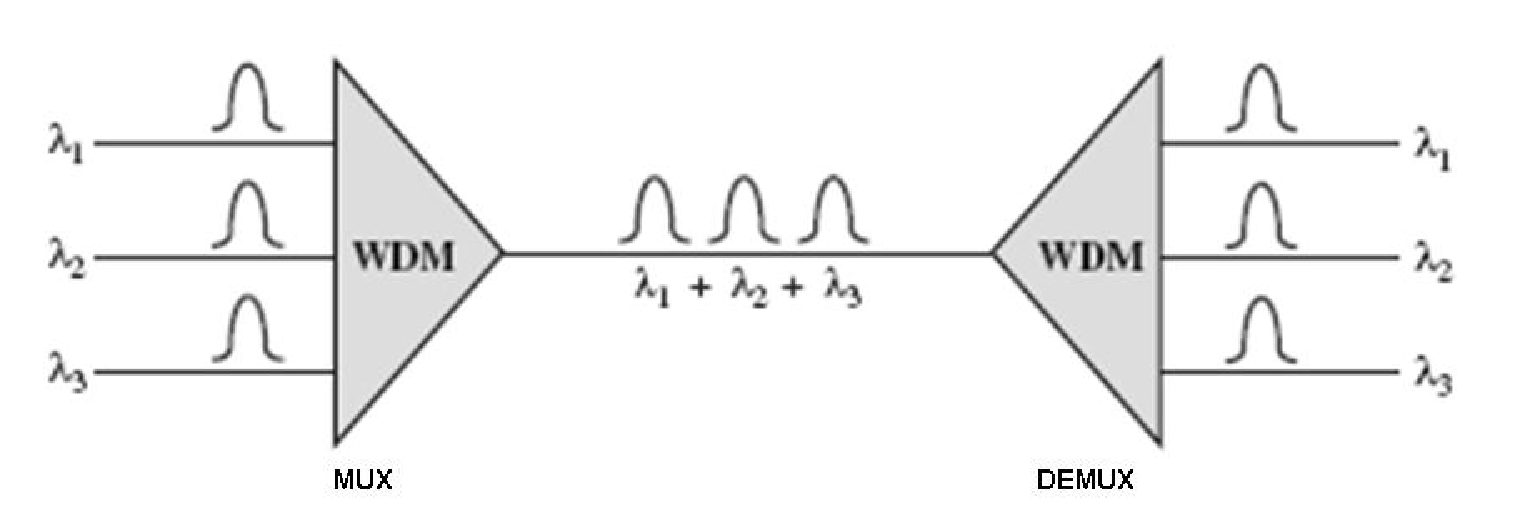
\includegraphics[scale=.5]{./figs/mux-demux.eps}
 % mux-demux.eps: 0x0 pixel, 300dpi, 0.00x0.00 cm, bb=0 0 713 239
 \caption{Multiplexa��o e Demultiplexa��o em um sistema WDM.}
 \label{fig:mux-demux}
\end{figure}


Um componente b�sico das redes com roteamento por comprimento de onda, conhecido como \textit{Wavelength Crossconect} (WXC) ou \textit{Wavelength Routing
Switch}, tem a fun��o de
permitir a conex�o (�ptica) de qualquer canal de entrada (comprimento de onda) em uma porta de entrada (fibra �ptica) com outra porta qualquer de sa�da ou a
retirada do canal para processamento. A figura \ref{fig:wxc} ilustra conceitualmente um WXC.

\begin{figure}[!ht]
 \centering
 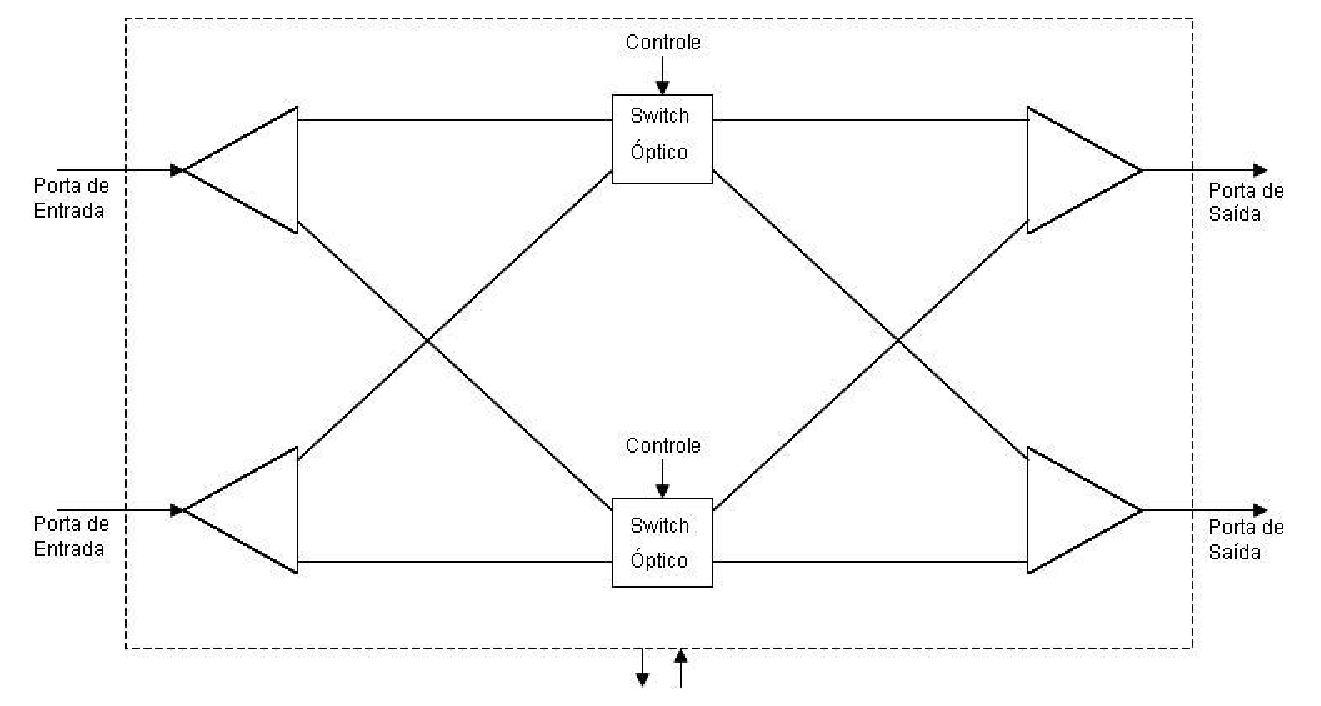
\includegraphics[scale=.6]{./figs/wxc.eps}
 % wxc.eps: 0x0 pixel, 300dpi, 0.00x0.00 cm, bb=0 0 618 323
 \caption{WXC com duas portas de entrada e duas portas de sa�da.}
 \label{fig:wxc}
\end{figure}

Um mecanismo comum para transmiss�o em sistemas �pticos � constituido pelo uso de \textit{lasers} semicondutores como fontes de luz. Os transmissores usados em
redes WDM
geralmente requerem a possibilidade de sintonia em diferentes comprimentos de onda.

% %%%%%%%%%%%%%%%%%%
% Em uma rede WDM com roteamento por comprimento de onda o meio de comunica��o utilizado para estabelecer uma conex�o � chamado caminho �ptico. Para
% estabelecer
% uma conex�o entre um par de n�s fonte e destino, � utilizada uma rota cont�nua para um comprimento de onda entre este par de n�s. Um algoritmo para a sele��o
% de
% rotas e comprimentos de onda para o estabelecimento de caminhos �pticos � chamado de RWA - Routing and Wavelength Assignment Algorithm.
% A demanda por conex�es ou demanda de tr�fego, pode ser est�tica ou din�mica. Neste trabalho estudamos apenas o caso de demanda est�tica de tr�fego, onde o
% mesmo
% � conhecido ou estimado a priori. O objetivo do RWA � definir as rotas e alocar os comprimentos de onda de forma a atender toda a demanda de tr�fego
% utilizando
% o menor n�mero poss�vel de comprimentos de onda.
% %%%%%%%%%%%%%%%%%%
% 
% %%%%%%%%%%%%%%%%%%
% A topologia virtual ou l�gica em uma rede, definida no dom�no �ptico, � formada por um conjunto de caminhos �pticos estabelecidos entre os pares de n�s da
% rede.
% Em uma topologia virtual, se dois n�s s�o conectados por um caminho �ptico, eles podem se comunicar atrav�s de um salto l�gico ou �ptico. Devido a limita��es
% tecnol�gicas e financeiras, refletidas no n�mero de comprimentos de onda e transmissores/receptores, em geral n�o � poss�vel ou de interesse estabelecer
% caminhos �pticos entre todos os pares de n�s de uma rede. Se dois n�s n�o s�o conectados diretamente por um caminho �ptico, eles poder�o se comunicar atrav�s
% de
% uma sequ�ncia de caminhos �pticos, sendo as demandas de tr�fego processadas eletronicamente entre dois caminhos �pticos consecutivos. Este tipo de comunica��o
% �
% chamada de multi-salto.
% 
% O tr�fego entre os pares de n�s � roteado sobre a topologia virtual em um ou mais saltos. A topologia pe projetada visando otimizar m�tricas de qualidade,
% como
% atraso m�dio ou congestionamento. O atraso m�dio pode ser medido em termos do n�mero de saltos l�gicos ou pelas dist�ncias f�sicas associadas aos mesmos. O
% congestionamento da rede � definido como a maior quantidade de tr�fego em um caminho �ptico da rede. � importante destacar que um caminho �ptico pode carregar
% tr�fego associado a diferentes pares de n�s.
% %%%%%%%%%%%%%%%%%%

%\section{Redes �pticas com Roteamento por Comprimento de Onda}

Conforme descrito em \cite{murthy}, uma rede com roteamento por comprimento de onda (WRON - {\it Wavelength Routed Optical Networks}) consiste em WXCs, n�s
roteadores, interconectados por enlaces �pticos ponto-a-ponto formando uma topologia. Cada n� terminal � conectado a um WXC atrav�s de uma fibra �ptica. A
combina��o de um n� terminal com seu correspondente WXC � referida, de forma geral, como n� (da rede). Cada n� � equipado com um conjunto de transmissores e
receptores, todos com capacidade de sintonia de comprimento de onda.

Os dados s�o enviados de um n� para outro usando uma rota cont�nua, com um �nico comprimento de onda, chamada de caminho �ptico, n�o requerendo
qualquer convers�o eletro-�ptica ou armazenamento em fila nos n�s intermedi�rios. Este processo � conhecido como roteamento por comprimento de onda. Destaca-se
que os n�s intermedi�rios roteiam os caminhos �pticos no dom�nio �ptico usando seus WXCs. Os n�s terminais de um caminho �ptico o acessam por meio de
transmissores (in�cio) e receptores (fim), de forma gen�rica chamados de tranceptores, que s�o sintonizados para o comprimento de onda no qual o caminho �ptico
opera. Cada caminho �ptico � associado a uma
rota f�sica e a um comprimento de onda. O requisito de que um mesmo comprimento de onda deve ser usado ao longo de todos os enlaces que comp�em um caminho
�ptico
� conhecido como restri��o de continuidade de comprimento de onda. Dois caminhos �pticos n�o podem assumir o mesmo comprimento de onda em uma fibra,
este requisito � conhecido como restri��o de atribui��o de comprimentos de onda distintos. No entanto, dois caminhos �pticos podem usar o mesmo
comprimento de onda se eles percorrem conjuntos disjuntos de enlaces f�sicos, essa propriedade � conhecida como reutiliza��o de comprimentos de onda.

Uma rede �ptica com roteamento por comprimento de onda pode ser utilizada no roteamento de pacotes, para tanto, um conjunto de caminhos �pticos, representando a
camada �ptica da rede, s�o definidos sobre a sua camada f�sica atrav�s da configura��o dos WXCs em cada n�. Dessa forma, um pacote proveniente de um n� fonte,
pode ser transmitido at� um n� intermedi�rio atrav�s de um caminho �ptico, ser processado eletronicamente e posteriormente retransmitido para um caminho �ptico
subsequente, formando uma rota at� alcan�ar seu n� de destino.

Se uma rede WDM entrega informa��o diretamente no dom�nio �ptico para todos os pares de n�s, ela � conhecida com uma Rede Totalmente �ptica (WRAN -
\textit{Wavelength Routed All-Optical Network}). Uma vantagem deste tipo de rede � evitar atrasos e perdas com convers�es eletro-�pticas, processamento
eletr�nico e filas. A principal desvantagem est� na limita��o tecnol�gica e financeira em estabelecer caminhos �pticos entre todos os pares de n�s da rede.


%\section{Topologias F�sica e Virtual}

Os conjuntos de n�s e enlaces f�sicos (fibras �pticas) constituem a topologia f�sica. Enquanto o conjunto de caminhos �pticos definidos sobre a
topologia f�sica formam a topologia virtual ou l�gica. Na topologia virtual, os n�s correspondem aos pr�prios n�s da rede e as arestas aos caminhos �pticos. O
grau l�gico de entrada de um n� na topologia virtual � definido como o n�mero de caminhos �pticos que incidem no n�, enquanto o grau l�gico de
sa�da como o n�mero de caminhos �pticos que partem do mesmo. Os graus l�gicos de entrada e sa�da de um n� s�o limitados pelo n�mero de receptores
e transmissores �pticos dispon�veis no n�, respectivamente. E ainda, considerando $ W $ o n�mero de comprimentos de onda dispon�veis por enlace f�sico e
$D_{in}^{f} $ e $ D_{out}^{f} $ os graus f�sicos de entrada e sa�da de um n�, respectivamente. Em uma topologia virtual o grau l�gico de entrada ($ D_{in}^{v}
$) deste n� pode ser no m�ximo $ W $ x $ D_{in}^{f} $ e seu grau l�gico de sa�da ($ D_{out}^{v} $) pode ser no m�ximo $ W $ x $ D_{out}^{f} $.


%\section{Roteamento de Tr�fego pela Topologia Virtual}

Para o roteamento de tr�fego pela topologia virtual, se dois n�s est�o conectados por uma aresta na topologia virtual, uma demanda pode ser transmitida de um n�
a outro no dom�nio �ptico, sem requerer qualquer convers�o eletro-�ptica em n�s intermedi�rios. Neste caso, a demanda � roteada em um salto virtual (l�gico). Um
WXC � usado para direcionar (no dom�nio �ptico) a demanda que chega ao n� intermedi�rio para um enlace de sa�da sem processamento de informa��o no n�. Uma
demanda requer processamento eletr�nico em um n� em duas situa��es: a demanda precisa ser destinada a um n� que n�o est� conectado diretamente ao seu n� fonte
atrav�s de um caminho �ptico ou a demanda precisa ser recebida pelo seu n� destino. Uma demanda chegando a um n� no dom�nio �ptico � convertida para sua forma
eletr�nica e armazenada. Caso o n� de destino desta demanda seja outro, ela � convertida novamente para o dom�nio �ptico e transmitida por um enlace de sa�da.
Por outro lado, se ela for destinada para o n� atual, ela � entregue eletronicamente para a camada superior da rede.


%\section{Projeto de Redes �pticas Semitransparentes}

O projeto e planejamento de redes � realizado atrav�s de m�todos distintos de acordo com o tipo de tr�fego considerado, especificamente com rela��o a natureza
est�tica ou din�mica. No caso de tr�fego est�tico, nosso foco de estudo, � assumido a priori uma determinada matriz de demanda de tr�fego, representando a
quantidade de tr�fego que deve ser transferido entre os pares de n�s da rede. Considera-se essas demandas como sendo fixas para fins de planejamento, podendo
basear-se em levantamentos hist�ricos ou mesmo estudos estimativos. N�o ser�o consiredadas aqui a poss�bilidade de bloqueio de pacotes e nem outros tipos de
perdas na transmiss�o. Portanto, � assumido que todo o tr�fego da rede ser� devidamente enviado e recebido.

Uma rede �ptica � transparente quando n�o existe regenera��o eletr�nica dos caminhos �pticos durante o seu percurso fim-a-fim, enquanto uma rede �ptica � opaca
quando cada caminho �ptico � regenerado em todos os n�s pelo qual transita na rede. Uma rede �ptica transparente n�o tem apenas restri��es relacionadas
com degrada��es acumuladas, mas tamb�m com monitora��o de performance, isola��o de falhas, gerenciamento centralizado, continuidade de comprimento de onda,
entre
outras \cite{bala00}. Usando redes �pticas semitransparentes, � poss�vel alcan�ar uma performance muito pr�xima aos das redes opacas em termos de bloqueio de
novas requisi��es, por�m com grande economia nos custos, e menos complexidade do que uma rede completamente �ptica. Em suma, redes semitransparentes, foco
do presente trabalho, oferecem o
melhor dos dom�nios �pticos e eletr�nicos sem comprometer as principais caracter�sticas de cada uma dessas tecnologias \cite{bala00}.

O projeto de WRONs deve levar em conta seus custos de implementa��o e opera��o, que podem ser colocados, resumidamente, em fun��o dos recursos de
transmiss�o requeridos na camada �ptica e a capacidade de processamento e armazenamento dos roteadores eletr�nicos. Para tanto, t�cnicas de
otimiza��o s�o largamente empregadas e as solu��es propostas fazem uso de m�todos exatos e heur�sticas, separadamente ou em conjunto. Na literatura
\cite{ram02}, o projeto completo de WRON � dividido em quatro sub-problemas, que s�o denominados: roteamento de tr�fego  (TR -
\textit{Traffic Routing}), projeto da topologia l�gica (LTD - \textit{Logical Topology Design}), roteamento de comprimentos
de onda (WR - \textit{Wavelength Routing}) e aloca��o de comprimentos de onda (WA - \textit{Wavelength Assignment}).

\begin{figure}[htb]
\centering
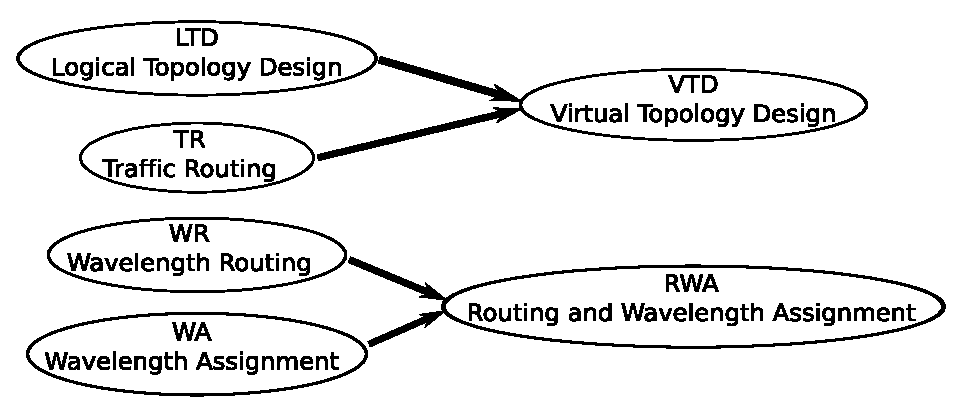
\includegraphics[bb=76 270 522 453, scale=.9]{figs/4subprob.eps}
% 4subprob.eps: 0x0 pixel, 300dpi, 0.00x0.00 cm, bb=76 270 522 453
\caption{Quatro sub-problemas se fundem em VTD e RWA.}
\label{fig:4subprob}
\end{figure}

Tradicionalmente, os dois primeiros sub-problemas s�o associados, bem como os dois �ltimos, compondo, respectivamente, os conhecidos problemas de
VTD (\textit{Virtual Topology Design}) \cite{ram02} e RWA (\textit{Routing and Wavelength Assignment}) \cite{Zang00}. Isto est� ilustrado na figura
\ref{fig:4subprob}.

Em resumo, o VTD pode ser descrito como a defini��o da topologia virtual da rede e posterior distribui��o do tr�fego pelo mesma. Tendo como dados de entrada, a
matriz de demandas de tr�fego e o grau l�gico considerado. Duas das principais m�tricas controladas ou otimizadas pelo VTD s�o o congestionamento e o tr�fego
retransmitido pelos n�s \cite{Renato06}. O congestionamento representa o total de tr�fego alocado ao caminho �ptico mais carregado da rede. O congestionamento
pode ser entendido como a necessidade de capacidade de transmiss�o dos caminhos �pticos, pois para se atender � demanda de tr�fego, � necess�rio que essa
capacidade seja no m�nimo igual ao congestionamento calculado. O tr�fego retransmitido pelos n�s � uma caracter�stica das redes semitransparentes, pois �
definido como a soma das demandas de tr�fego que chegam e saem dos n�s intermedi�rios das rotas de comunica��o entre os pares de n�s da rede. Esse tr�fego
possui impacto direto sobre a capacidade de processamento eletr�nico dos n�s, e dessa forma sobre o seu custo, pois ele representa as demandas recebidas,
processadas eletronicamente e encaminhadas novamente para o n� seguinte da rota.

O RWA \cite{Zang00} pode ser descrito como a defini��o das rotas f�sicas dos caminhos �pticos e posterior aloca��o de comprimentos de onda aos mesmos. Possui
como dados de entrada uma matriz de requisi��es, que pode ser entendida como a pr�pria topologia virtual, al�m da topologia f�sica da rede. O objetivo principal
� utilizar o menor n�mero poss�vel de comprimentos de onda para atender a todas as requisi��es.





%%%%%%%%%%%%%%%%%%%%%%%%%%%%%%%%%%%%%
%% Revis�o Bibliogr�fica
%% Copyright 2009 Marcelo de Oliveira Lima.
%% Este documento � distribu�do nos termos da licen�a 
%% GNU General Public License v2.
%%%%%%%%%%%%%%%%%%%%%%%%%%%%%%%%%%%%%


\chapter{Trabalhos Anteriores}
\label{review}

Este cap�tulo faz um apanhado geral dos trabalhos encontrados na literatura que abordam o projeto de redes �pticas. O problema de projetar uma rede �ptica pode
ser formulado como um problema de programa��o inteira mista (MILP), sendo definida uma m�trica de interesse a ser otimizada. Esse problema j� foi amplamente 
estudado, muitas vezes recorrendo-se ao uso de m�todos heur�sticos para resolv�-lo, sendo conhecidamente NP-dif�cil. As diferentes abordagens partem de
considera��es espec�ficas sobre as demandas de tr�fego, tipo de topologia, capacidade de convers�o de comprimentos de onda, m�trica a ser otimizada, entre
outras. Quando as demandas de tr�fego s�o assumidas como sendo est�ticas, caso adotado neste trabalho,  todas as demandas  a serem transmitidas entre os pares
de n�s da rede s�o conhecidas a \textit{priori} e fixas. Neste caso, o objetivo normalmente � a minimiza��o de algum recurso da rede, tendo como exemplos:
n�mero de
comprimentos de onda utilizados, capacidade dos canais de comunica��o, n�mero de tranceptores e processamento eletr�nico. Com uma frequ�ncia menor, tamb�m
s�o
encontrados trabalhos que abordam o projeto da topologia f�sica da rede, ou seja, a defini��o dos pares de n�s que possuir�o enlaces de fibra �ptica
interligando-os diretamente, neste caso de estudo o objetivo em geral � a minimiza��o de um par�metro de custo de instala��o da rede, que normalmente varia
entre o n�mero de enlaces necess�rios ou o comprimento total de enlaces a serem instalados, existindo tamb�m casos onde se considera m�tricas como o n�mero de
comprimentos de onda ou de tranceptores previstos. 

Os trabalhos encontrados na literatura em geral resolvem parte dos subproblemas que constituem o projeto de uma WRON, dessa forma, as descri��es
apresentadas a seguir ressaltam as diferentes abordagens existentes.

O projeto de uma topologia virtual foi formulado como um problema de otimiza��o em \cite{Mukherjee96}. Os autores formularam o problema atrav�s de um modelo de
otimiza��o n�o linear. A fun��o objetivo considerava a minimiza��o do atraso na transmiss�o e do m�ximo fluxo em um enlace, sendo este �ltimo conhecido como o
congestionamento da rede. Os autores subdividem o problema em quatro subproblemas: 1) determina��o da topologia l�gica; 2) roteamento dos caminhos �pticos sobre
a topologia f�sica; 3) aloca��o de comprimentos de onda �s rotas; 4) roteamento das componentes de tr�fego na topologia l�gica. Nos experimentos
apresentados, os autores consideram apenas os subproblemas 1 e 4. Para a realiza��o de experimentos, foi desenvolvido um m�todo que emprega a meta-heur�stica
\textit{Simulated Annealing}. Posteriormente na literatura, o problema representado pelos subproblemas 1 e 4 conjuntamente passou a ser conhecido como
$VTD$ (\textit{Virtual Topology Design}), possuindo varia��es na fun��o objetivo considerada. Em \cite{ram96} os autores formularam uma modelagem MILP para
resolu��o do $VTD$ tamb�m com o objetivo de minimizar o congestionamento. N�o existe restri��o
quanto ao n�mero de comprimentos de onda utilizados. Nesta abordagem a topologia f�sica torna-se irrelevante para o projeto da topologia l�gica, pois n�o �
resolvido o $RWA$ (\textit{Routing and Wavelength Assignment}). O tr�fego retransmitido na rede foi assumido como fun��o objetivo em \cite{Renato06},
enquanto o congestionamento era controlado atrav�s de uma restri��o na formula��o matem�tica utilizada. Conforme ser� detalhado no cap�tulo \ref{metodo}, a
metodologia desenvolvida no presente trabalho limita o congestionamento e o tr�fego retransmitido na rede
baseando-se em exig�ncias de qualidade estimadas por meio de infer�ncia estat�stica.

% Em \cite{Banerjee00} � apresentada uma forma��o MILP para o projeto da topologia virtual de redes �pticas WDM com convers�o de comprimentos de onda. O
%objetivo
% neste trabalho era minimizar a dist�ncia m�dia dos saltos dos pacotes de dados. Foi adotado tr�fego baseado em pacotes. A formula��o MILP apresentada,
%inclui a
% defini��o dos caminhos �pticos, seu roteamento f�sico e a aloca��o de tr�fego sobre os mesmos. Com o objetivo de tornar o problema trat�vel, a restri��o
%de
% continuidade de comprimentos de onda foi relaxada, considerando que todos os n�s possuem capacidade de convers�o. Devido a dificuldade de obter solu��es
% �timas
% com o modelo, nos experimentos, o processo de otimiza��o foi interrompido ap�s um determinado n�mero de itera��es.


Em \cite{Sivarajan01} � proposta uma modelagem MILP que minimiza congestionamento em redes sem conversores de comprimentos de onda. Segundo os autores, esta
formula��o n�o � computacionalmente trat�vel, sendo m�todos heur�sticos propostos. O modelo MILP � relaxado e executado iterativamente por $25$ vezes usando um
plano de corte. As vari�veis que representam a topologia virtual e os percursos f�sicos s�o arredondadas, enquanto uma heur�stica de aloca��o de comprimentos de
onda � aplicada para atribuir comprimentos de onda individualmente aos caminhos �pticos. O tr�fego � roteado pela topologia virtual utilizando uma formula��o
linear (LP) consistindo somente das restri��es de tr�fego do MILP relaxado. Uma desvantagem desse m�todo, � que supondo que existam $W$ comprimentos de onda
dispon�veis em cada fibra, o MILP relaxado obt�m uma solu��o que satisfaz esta restri��o. No entanto, na execu��o do algoritmo de aloca��o de comprimentos de
onda, que � aplicado posteriormente e obt�m solu��es sub-�timas, n�o h� garantia de uma aloca��o de comprimentos de onda com sucesso, respeitando o limite
$W$. Como resultado, o m�todo n�o retorna necessariamente solu��es vi�veis para todos os casos. O modelo proposto � dos mais abrangentes da literatura,
sendo que a �nica etapa do projeto de WRON n�o resolvida � a escolha da topologia f�sica. Assim como no presente trabalho, a formula��o permite a cria��o
de m�ltiplos caminhos �pticos entre um mesmo par de n�s da rede.

% Algumas heur�sticas para o projeto de redes �pticas foram apresentadas em \cite{Nina05}. Este trabalho envolve o projeto de topologias virtuais
% sem utiliza��o de conversores de comprimento de onda. O m�todo proposto utiliza uma heur�stica e � avaliado atrav�s de possibilidades variadas de fun��es
% objetivo, sendo analisadas as vantagens e desvantagens para cada crit�rio de otimiza��o.  Os resultados apresentados foram gerados para redes de tamanhos
% variados e para caracter�sticas de tr�fego uniforme e n�o uniforme.


% Em \cite{Banerjee97}, os autores formularam o problema de projeto de topologia l�gica como um problema linear que considera os n�s da rede equipados com
% conversores de comprimento de onda. A fun��o objetivo da formula��o � a minimiza��o do comprimento dos saltos nos enlaces l�gicos, com a possibilidade de
%redu��o
% do n�mero de conversores de comprimentos de onda utilizados e, dessa forma, esta formula��o poderia ser aproximada para uma formula��o sem convers�o. As
% defici�ncias desta formula��o s�o: 1) ela produz resultados razo�veis somente se a matriz de tr�fego for equilibrada, sendo esta uma consequ�ncia da fun��o
% objetivo n�o incluir vari�veis de tr�fego; 2) trabalha bem somente se a topologia f�sica for densa em termos do n�mero de arestas. Note que se a topologia
%f�sica
% for esparsa (com poucas arestas) ent�o o n�mero de conversores de comprimento de onda utilizados aumentar� (poucas rotas alternativas) e a topologia l�gica
% resultante pode n�o refletir o tr�fego entre os n�s. A restri��o de continuidade dos comprimentos de onda n�o foi utilizada nesta formula��o.


% O RWA tamb�m � explorado em \cite{Zang00}, este estudo detalha o problema de roteamento e aloca��o de comprimentos de onda em redes WDM com a restri��o de
% continuidade de comprimentos de onda, ou seja, n�o utilizam conversores. � apresentada uma revis�o de v�rias abordagens e m�todos apresentadas na
%literatura,
% abrangendo modelagens MILP e heur�sticas.

Um modelo MILP foi apresentado em \cite{Karcius04}. Este trabalho prop�e um algoritmo iterativo, que faz uso de programa��o linear, para resolver os problemas
VTD e RWA de forma integrada. A topologia l�gica � escolhida com a heur�stica $HLDA$ \cite{ram96}, e esse resultado � fixado no modelo proposto. O modelo �
resolvido para encontrar solu��o para as demais vari�veis. Por se tratar de um modelo MILP de alto custo computacional, a resolu��o � interrompida depois de
um tempo pr� determinado. A fun��o objetivo adotada foi o n�mero total de saltos nas rotas f�sicas. A estrat�gia foi passar ao modelo limita��es para as
m�tricas importantes, de modo que as solu��es vi�veis encontradas fossem satisfat�rias. Essa abordagem torna-se �til dada a abrang�ncia do modelo proposto,
onde m�tricas dos sub-problemas do projeto de uma WRON podem ser controladas.  Todavia o alto custo computacional do modelo proposto inviabiliza sua
aplica��o para redes de grande porte. As redes testadas tinham 6 e 12 n�s. No presente trabalho esta estat�gia de definir exig�ncias de qualidade para
m�tricas de interesse e a heur�stica $HLDA$ tamb�m ser�o empregadas, conforme est� apresentado no cap�tulo \ref{metodo}.

\section{Topologia F�sica}

Em \cite{bannister90} foi desenvolvida uma formula��o para o projeto de redes WDM e analisados os princ�pios deste tipo de rede. O autor constatou a
ocorr�ncia de interfer�ncias entre o projeto das topologias virtual e f�sica,
considerando a qualidade da topologia virtual relacionada � par�metros de performace da rede. A qualidade da topologia f�sica foi relacionada ao custo de
instala��o, representado pelos comprimentos dos enlaces de fibra �ptica. Adotou-se como objetivo minimizar o atraso m�dio de pacotes. Assim como em nosso
trabalho, o autor utiliza uma matriz de demanda de tr�fego que especifica a taxa, por exemplo em pacotes por segundo, na qual o tr�fego � transmitido entre
os pares de n�s da rede, ao inv�s de requisi��es entre os pares de n�s. O foco principal  � a escolha das melhores topologias f�sica e virtual poss�veis
mediante um conjunto de par�metros de rede estabelecidos. N�o � resolvida a aloca��o de comprimentos de onda.

O trabalho \cite{Tornatore07} trata de m�todos exatos para o planejamento e otimiza��o de redes WDM multi-fibras, ou seja, foi contemplada a cria��o de mais
de um enlace de fibra entre um par de n�s, diferentemente do presente trabalho. O autor prop�e uma formula��o para o problema
chamada de \textit{source formulation}, nela todo o fluxo � agregado em rela��o ao n� de origem. Esta formula��o � equivalente � cl�ssica, denominada
\textit{flow formulation}, por�m permite uma redu��o relevante no n�mero de vari�veis e restri��es, representando uma redu��o no tempo computacional durante
a
execu��o. O modelo $TWA$ que ser� apresentado no pr�ximo cap�tulo possui semelhan�as conceituais quanto a agrega��o de tr�fego. Com rela��o a convers�o de
comprimentos de onda, os casos extremos s�o tratados, quando todos os n�s possuem capacidade de converter todos os
comprimentos de onda, e quando nenhum n� possui capacidade de convers�o, sendo exigida a restri��o de continuidade. O trabalho prop�e a otimiza��o da
topologia
virtual de uma rede f�sica multi-fibra, com o objetivo de minimiza��o de custo. O n�mero de fibras por enlace necess�rias para suportar uma matriz de
tr�fego
pr�-estabelecida � especificamente a vari�vel a ser minimizada, tendo como dado de entrada o n�mero de comprimentos de onda por fibra. 


O projeto de redes totalmente �pticas com roteamento por comprimento de onda (WRAN) foi estudado em \cite{liu2008}. O autor o abordou a necessidade de
decis�o entre a instala��o de mais fibras ou o aumento do n�mero de comprimentos de onda utilizados. Ambas alternativas podem ser empregadas para
suportar novas conex�es, no entanto, uma eleva o custo de enlaces e a outra o dos n�s, este �ltimo representado pelos equipamentos usados nos mesmos. Foi
apresentado um algoritmo que busca solu��es que minimizam o custo total para a topologia f�sica, para tanto, empregou-se uma formula��o matem�tica para o
problema, al�m de um algoritmo heur�stico. Segundo o autor, na instala��o de uma WRAN � importante avaliar alternativas visando minimizar o capital
investido, sendo o custo total dividido entre enlaces e n�s. O custo dos enlaces est� relacionado � instala��o das
fibras para interligar os n�s da rede e � uma fun��o do comprimento total dos enlaces. O custo relativo aos n�s, � representado pelos roteadores de
comprimentos de onda e � fun��o do n�mero de comprimentos de onda utilizados em cada enlace. Seria poss�vel formar uma topologia f�sica usando uma
quantidade m�nima de fibra a partir de uma �rvore geradora m�nima (\textit{Minimum Spanning Tree}), no entanto esta configura��o implicaria em um custo
elevado para os n�s, pois seria necess�rio uma grande quantidade de comprimentos de onda. Em outro extremo, seria poss�vel conectar todos os pares de n�s
atrav�s de enlaces diretos. Isto implicaria em um custo m�nimo para os n�s, por�m um alto custo para os enlaces. Foi apresentada uma formula��o matem�tica e
nos experimentos foi analisada a rela��o entre o custo dos n�s e dos enlaces visando fornecer aos projetistas de redes uma ferramenta para o projeto de
redes com boa qualidade t�cnica e financeira. Os conceitos abordados s�o aplic�veis a WRON, desde que sejam feitas as devidas considera��es relativas �s
especificidades decorrentes da necessidade de retransmiss�o.

O projeto de topologia f�sica para WRAN tamb�m foi estudado em \cite{xiao}. No problema abordado, � conhecido o n�mero de requisi��es entre
os pares de n�s e as especifica��es de custo para estabelecer um enlace f�sico entre cada par de n�s, tendo como objetivo determinar a topologia de
menor custo para a rede. � apresentada uma formula��o do problema, provado que se trata de um problema NP-completo e desenvolvido um algoritmo chamado
\textit{Two-Stage Cut Saturation}. Em um primeiro momento, � relaxada a restri��o de continuidade de comprimentos de onda e aplicado o princ�pio de \textit{Cut
Saturation} para determinar uma solu��o inicial para a rede. Em seguida, no segundo est�gio, � inserida a restri��o de continuidade de comprimentos de onda e
resolvido o RWA para atender �s requisi��es sobre a rede gerada inicialmente. Al�m da escolha da topologia f�sica, este estudo possui semelhan�a com a
metodologia apresentada no cap�tulo \ref{metodo} devido a resolu��o do problema por etapas.

Os autores de \cite{guan} abordam o projeto de topologias f�sica e l�gica, analisando diferentes tipos de arquiteturas de redes. O custo das solu��es s�o
avaliados pelo n�mero de enlaces de fibras utilizados e por uma modelagem de custo relacionado aos OXCs. Foi demonstrada a relev�ncia dos saltos l�gicos com
rela��o ao dimensionamento dos recursos de roteamento, al�m de analisada a influ�ncia do grau dos n�s sobre o desempenho das solu��es.

\section{Topologia em Hierarquia}

Foi proposta em \cite{fonseka} uma arquitetura de hierarquia em an�is chamada \textit{Hierarchical Self-Healing Rings} (HSHR) e o projeto dessas redes
explorado. A arquitetura HSHR consiste de an�is em n�veis diferentes, sendo que um anel de n�vel superior � usado para conectar os an�is imediatamente
inferiores, de forma que cada anel em um determinado n�vel somente se comunica diretamente a um �nico anel de n�vel imediatamente superior. Um modelo geral
de custo incorporando materiais e instala��o foi usado. Mostrou-se que o m�todo de enumera��o, que encontra a configura��o �tima para a rede, somente pode
ser utilizado para redes de pequeno porte devido a complexidade. S�o apresentadas heur�sticas para encontrar solu��es de qualidade para a configura��o dos
HSHR. O roteamento e dimensionamento dos an�is tamb�m s�o considerados.

Conforme descrito em \cite{peng} uma modelagem de rede em hierarquia pode reduzir a complexidade do roteamento e aloca��o de comprimentos de onda (RWA) em
redes WDM quando comparados a modelos para redes em malha. No entanto, a utiliza��o de recursos pode ser ineficiente se a arquitetuta em hierarquia n�o for
adequadamente planejada. Partindo do grau de cada n� e do impacto da localiza��o, neste trabalho foi proposto um m�todo heur�stico para constru��o de
topologias em hierarquia para redes WDM visando a maximiza��o da utiliza��o dos recursos de rede. A topologia da rede em hierarquia � obtida pelo agrupamento
de n�s com seus respectivos n�s LRA (\textit{Local Routing Area Node}), sendo que a interconex�o dos n�s LRA constitue uma hierarquia de
n�vel superior. Com uma solu��o focada no desempenho do RWA, foram observados os resultados para a quantidade de comprimentos de onda utilizados,
assumindo que cada enlace de fibra possui quatro comprimentos de onda dispon�veis. A rede utilizada nos testes possui $28$ n�s. Foram avaliados diferentes
m�todos de roteamento e analisada a taxa de bloqueio na rede.


%%%%%%%%%%%%%%%%%%%%%%%%%%%%%%%%%%%%%
%% Modelagem TWA
%% Copyright 2009 Fabio de Oliveira Lima.
%% Este documento � distribu�do nos termos da licen�a 
%% GNU General Public License v2.
%%%%%%%%%%%%%%%%%%%%%%%%%%%%%%%%%%%%%


\chapter{TWA - Modelo para o Projeto Completo de uma WRON }
\label{Basic}

Neste cap�tulo ser� apresentada a forma b�sica do modelo TWA (\textit{Traffic over Wavelength Assignment}), come�ando pela nota��o designada aos n�s e as
constantes que definem uma inst�ncia de
problema para o modelo. Em seguida ser�o definidas as vari�veis utilizadas para compor as restri��es e a fun��o objetivo do modelo, passando-se
ent�o � sua descri��o. A fun��o objetivo adotada na formula��o b�sica � a minimiza��o dos custos de instala��o e opera��o da rede, valendo-se da capacidade do
modelo escolher tamb�m a topologia f�sica da rede. Al�m disso, foi
considerada a restri��o de conserva��o dos comprimentos de onda ao longo do caminho �ptico \cite{Zang00}, ou seja, n�o se admite a convers�o de comprimentos de
onda na camada �ptica da rede nesta formula��o b�sica. Outros casos de uso e extens�es ao modelo b�sico ser�o apresentados no Cap�tulo \ref{cases}.

\section{Dados de Entrada e Vari�veis}

\begin{notation}
Para uma rede de $N$ n�s, os pares ordenados $(m,n)$, $(s,d)$ e $(i,j)$ indicam respectivamente liga��es f�sicas, demandas de tr�fego e liga��es l�gicas,
com $m\neq n$, $s\neq d$ e $i\neq j$, onde $m,n,s,d,i,j\in \{1,..,N\}$. O �ndice $w \in \{1,..,W\}$ representa comprimentos de onda, onde $W$ � a quantidade
limite de comprimentos de onda que podem ser usados. O �ndice $v\in \{1,..,N\}$ representa os n�s da rede.
\end{notation}

\begin{figure}[htb]
\centering
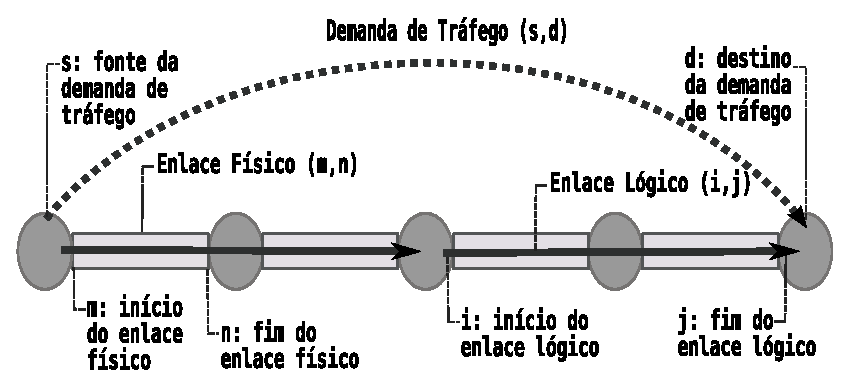
\includegraphics[bb=43 653 523 825,scale=.9]{figs/indices.eps}
\caption{Representa��o gr�fica da nota��o associada aos n�s da rede.}
\label{fig:Indices}
\end{figure}

A Figura \ref{fig:Indices} ilustra os diferentes escopos dos �ndices associados aos n�s da rede, com rela��o �s liga��es f�sicas $(m,n)$, liga��es l�gicas
$(i,j)$ e demandas de tr�fego $(s,d)$. Esta nota��o segue a conven��o comumente utilizada em trabalhos anteriores \cite{mukherjee,ram02}. �
importante dizer que esta modelagem suporta m�ltiplas liga��es f�sicas e l�gicas entre cada par de n�s, portanto, os pares $(m,n)$ e $(i,j)$ representam
conjuntos de poss�veis liga��es f�sicas e l�gicas, respectivamente. Esses conjuntos n�o ser�o explicitamente controlados, sendo esse um dos motivos
da simplicidade do modelo.

\begin{dados}
\label{Cons}
Uma inst�ncia para o modelo TWA � definida por:

\begin{enumerate}
\item $N$ $=$ N�mero de n�s da rede.
\item $W$ $=$ M�ximo de comprimentos de onda em uma liga��o f�sica.
% \item $H$ $=$ Grau f�sico m�ximo de entrada e sa�da de cada n�.
\item $K$ $=$ M�xima multiplicidade de liga��es f�sicas entre cada par $(m,n)$.
\item $Cap$ $=$ Capacidade de tr�fego de cada liga��o l�gica.
\item $C_{mn}$ $=$ Custo de uma liga��o f�sica entre o par $(m,n)$.
\item $T$ $=$ Custo por unidade de fluxo.
\item $P_{sd}$ $=$ Demanda de tr�fego, com origem $s$ e destino $d$.
\item $A_s = \sum_d P_{sd} =$ Tr�fego agregado pela origem $s$. 
\item $Q_{sd}=P_{sd}/A_s =$ Fra��o de $A_s$ correspondente � Demanda de tr�fego $P_{sd}$.
\end{enumerate}
\end{dados}

% \clearpage

 \subsection{Componentes Topol�gicos}
% \label{Top}

A vari�vel central do modelo, a partir da qual todas as demais ser�o definidas, chamada de componente topol�gico, � representada graficamente na Figura
\ref{fig:B} e formalmente definida na Vari�vel \ref{comp}. Ela sozinha representa as topologias l�gica e f�sica, as rotas f�sicas das 
liga��es l�gicas e os comprimentos de onda utilizados.

\begin{var}
\label{comp}
 Seja $B_{iw}^{mn} = k\in \{0,..,K\}$, com $i\neq n$, um componente do conjunto das liga��es l�gicas com origem $i$ e comprimento de onda $w$,
que utilizam $k$ liga��es f�sicas entre os n�s $m$ e $n$.
\end{var}

\begin{figure}[hbt]
 \centering
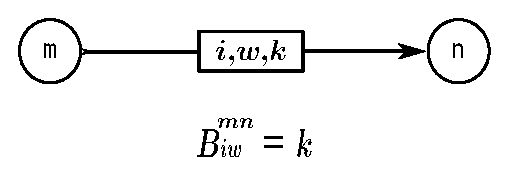
\includegraphics[bb=177 683 405 753, scale=0.9]{figs/B.eps}
% B.eps: 1179666x1179666 pixel, 300dpi, 9987.84x9987.84 cm, bb=36 739 246 805
 \caption{Representa��o gr�fica de um componente topol�gico.}
 \label{fig:B}
\end{figure}

Considerando que $B_{iw}^{mn}=k$ para algum $k \in \{0,..,K\}$, existem $k$ liga��es l�gicas originadas em $i$ no comprimento de onda $w$, passando
por $k$ liga��es f�sicas distintas entre o par de n�s $(m,n)$.  Conforme a terminologia utilizada
neste trabalho daqui por diante, \textit{um componente topol�gico $B_{iw}^{mn} = k$ � iniciado em $m$, incidente em $n$, com origem $i$,
comprimento de onda $w$ e valor $k$}.

Se $k>1$, ent�o h� multiplicidade de liga��es f�sicas entre o par de n�s $(m,n)$,
pois haveria interfer�ncia se houvessem duas liga��es l�gicas se propagando na mesma liga��o f�sica, com o mesmo comprimento de onda. Note
que $K$ limita apenas a multiplicidade das liga��es f�sicas, pois se $K=1$, $B_{iw}^{mn}$ se torna uma vari�vel bin�ria, mas ainda podem haver m�ltiplas
liga��es l�gicas entre um par $(i,j)$, utilizando rotas f�sicas distintas, ou ainda, comprimentos de onda diferentes em uma mesma
rota f�sica. Se $B_{iw}^{mn}=0$, $\forall\,(i,w)$, ent�o nenhuma liga��o f�sica entre o par de n�s $(m,n)$ � utilizada.

 Na Figura \ref{fig:Tops}, temos um exemplo de interpreta��o dos componentes topol�gicos, todos com origem no n� $v_1$ e com o 
mesmo comprimento de onda $w_1$. No item $d)$ desta figura, o valor $2$ do componente que liga os n�s $(v_1,v_2)$ � interpretado 
como duas liga��es f�sicas entre esses n�s, representadas no item $a)$. No item $b)$, vemos uma liga��o l�gica dupla entre os 
n�s $(v_1,v_3)$, onde uma delas passa de forma transparente pelo n� $v_2$, como indicado no item $c)$. Note ainda que, no item 
$d)$, h� dois caminhos l�gicos incidentes em $v_2$ mas apenas um iniciando. Isso indica que uma liga��o l�gica termina em $v_2$, 
enquanto a outra segue adiante.

% \clearpage
\begin{figure}[hbt]
 \centering
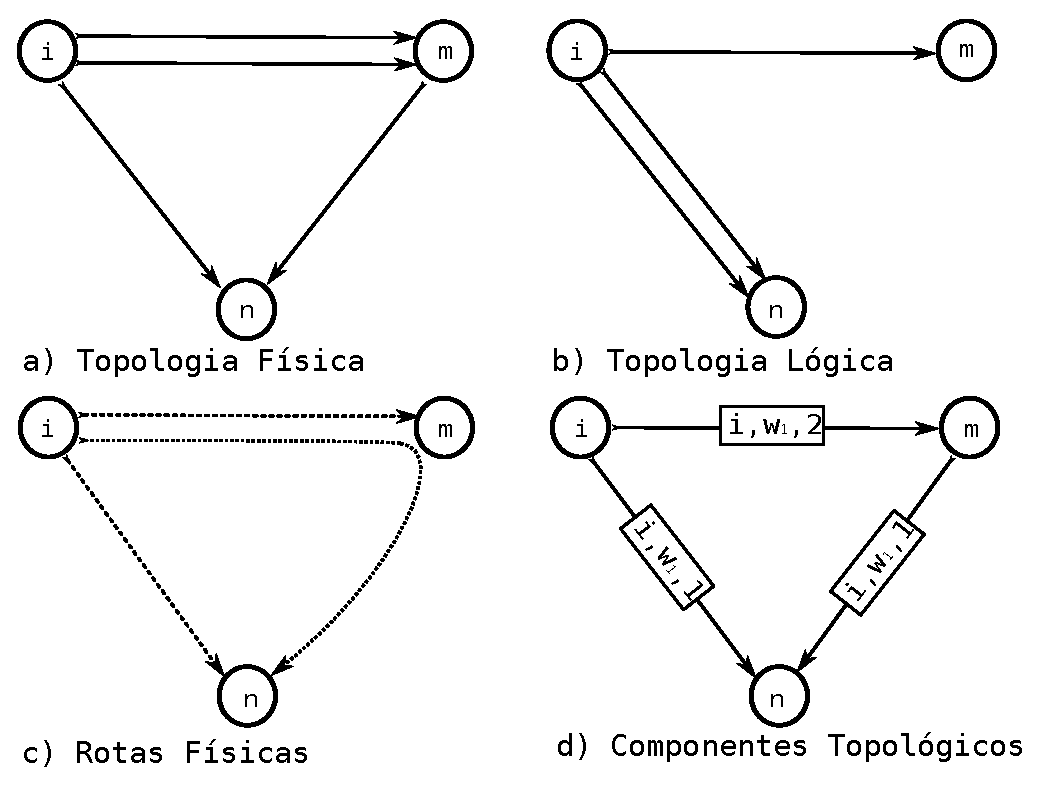
\includegraphics[width=0.8\textwidth]{figs/topologias-twa.eps}
% 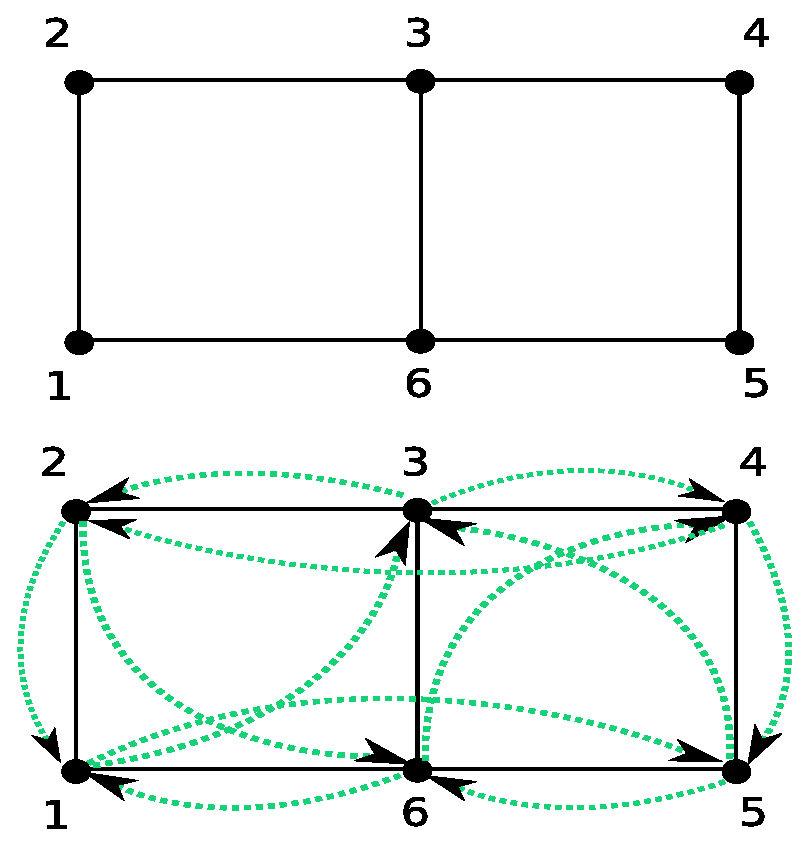
\includegraphics[bb=39 455 511 811, scale=0.4]{figs/topologias.eps}
 % topologias.eps: 1179666x1179666 pixel, 300dpi, 9987.84x9987.84 cm, bb=30 375 511 801
 \caption{Exemplo da interpreta��o dos componentes topol�gicos.}
 \label{fig:Tops}
\end{figure}
% \clearpage

A indexa��o atribu�da �s vari�veis $B_{iw}^{mn}$ especificam apenas o n� $i$ onde se iniciam as liga��es l�gicas representadas, sem deixar claro
aonde elas terminam. Isto significa que estas vari�veis agregam todas as liga��es l�gicas originadas em $i$ com comprimento de onda $w$, que utilizam as
liga��es f�sicas entre o par $(m,n)$, independente do n� $j$ em que terminam estas liga��es l�gicas. Esta t�cnica consiste em uma abordagem bastante
conhecida para a representa��o de vari�veis em problemas de distribui��o de fluxo em redes. Em \cite{Tornatore07}, este conceito de agrega��o de tr�fego �
aplicado como meio de simplifica��o do modelo, reduzindo substancialmente o n�mero de vari�veis dos problemas resultantes. No TWA, esta agrega��o cumpre o
mesmo papel de simplifica��o, cabendo �s restri��es do modelo garantir implicitamente a termina��o correta destas liga��es l�gicas agregadas nas vari�veis
$B_{iw}^{mn}$.

Para fins de compara��o entre modelos de programa��o inteira, usualmente uma vari�vel que pode assumir $K$
valores diferentes � convertida em $K$ vari�veis bin�rias \cite{cormen02}. A princ�pio, o n�mero de vari�veis bin�rias associadas aos componentes
topol�gicos seria $N^3\cdotp W\cdotp K$ \cite{cormen02}, mas devemos excluir algumas que s�o trivialmente nulas: aquelas com $i=n$, pois $i$ n�o pode ser
origem da liga��o l�gica e ao mesmo tempo destino da liga��o f�sica ($n$). Isso resulta em $N^3\cdotp W\cdotp K - N^2\cdotp K$.


\subsection{Fra��o de Fluxo das Demandas de Tr�fego}
\label{cap:twa-sec:VarFracFlow}

Para resolver o sub-problema de roteamento de tr�fego, � definida a vari�vel Vari�vel \ref{FlowVar}, que modela a fra��o de fluxo agregado para as
demandas de tr�fego. Elas s�o
semelhantes �s vari�veis de fluxo agregado utilizadas em \cite{ram96}, todavia h� duas diferen�as. Uma delas � que aqui essas vari�veis s�o normalizadas em
fun��o do tr�fego agregado na origem ($A_s$), e s�o portanto uma fra��o deste. Essa modifica��o n�o � requerida pela modelagem, tendo apenas a fun��o de
facilitar a compreens�o das restri��es do modelo, que ficam menos dependentes do dados de entrada. 

A outra diferen�a � que o fluxo � separado por comprimento de onda, como se fossem $W$ redes sem multiplexa��o sobrepostas. Isso facilita a interpreta��o
das
restri��es do modelo, e tamb�m ajuda a mant�-lo mais simples. De fato, o controle da distribui��o de fluxo deve ser feito em cada liga��o l�gica
\cite{ram02}, mas a restri��o de continuidade de comprimentos de onda exige uma equa��o para cada $w$ separadamente \cite{Zang00}. Soma-se a isso o fato de
que nesta modelagem m�ltiplas liga��es l�gicas s�o agregadas em cada par $(i,j)$ para todos os valores $w$ utilizados. Assim, separando o tr�fego por
comprimento de onda, foi poss�vel combinar o controle da distribui��o de tr�fego com a restri��o de continuidade de comprimentos de onda. Isso ser� tratado
com mais detalhes na Se��o \ref{cap:twa-sec:Bconserv_Cap}.

\begin{var}
 \label{FlowVar}
 Seja $q_{sw}^{ij} \in [0,1]$ a fra��o do fluxo originado em $s$, passando pelas liga��es l�gicas entre o par $(i,j)$ com comprimento de onda $w$,
onde $s\neq j$. 
\end{var}

Tamb�m devem ser exclu�das do modelo, por serem trivialmente nulas, as fra��es de fluxo com $s=j$. Pois $j$ � destino do tr�fego, n�o podendo ser ao mesmo
tempo origem ($s$). Assim, o n�mero de vari�veis reais associadas �s fra��es de fluxo � $N^3\cdotp W - N^2$.

\subsection{Topologia F�sica}
\label{cap:twa-sec:VarFis}

Apesar da topologia f�sica ser determinada pelos componentes topol�gicos, para fins de controle do custo de instala��o da rede f�sica,
s�o necess�rias novas inc�gnitas. Para este fim, � definida a Vari�vel \ref{FisVar}, que registrar� em $D_{mn}$ a multiplicidade f�sica determinada pelos
componentes topol�gicos. Se $D_{mn}=0$, n�o h� liga��es f�sicas entre o par $(m,n)$, mas se $D_{mn}=k$, para algum $k \in \{0,..,K\}$, existem $k$ liga��es
f�sicas entre o par $(m,n)$.

\begin{var}
\label{FisVar}
 Seja $D_{mn} \in \{0,..,K\}$ o n�mero de liga��es f�sicas entre o par de n�s $(m,n)$. 
\end{var}

O n�mero de vari�veis bin�rias associadas � $D_{mn}$ �  $N^2\cdotp K - N\cdotp K$ \cite{cormen02}, pois deve-se desconsiderar as vari�veis onde $m=n$. 

 \section{Custo de instala��o e Opera��o}
 \label{cap:twa-sec:funcaoobjetivo}


Duas m�tricas importantes no projeto da redes �pticas s�o os custos de instala��o e opera��o \cite{mukherjee}. 
O custo de instala��o $C_{mn}$ � o custo associado a uma liga��o f�sica entre o par de n�s $(m,n)$. O custo total de instala��o � dado na equa��o
\ref{eq:custoInstlacao}. O custo de opera��o $TO$, definido como o custo por unidade de fluxo, � calculado na equa��o \ref{eq:CustoDeOperacao}, e
influencia tamb�m no dimensionamento dos n�s da rede.

\begin{equation}
   CI = \sum_{mn} C_{mn}\cdot D_{mn}
   \label{eq:custoInstlacao}
\end{equation}


\begin{equation}
    TO = \sum_{sijw} T\cdot q_{sw}^{ij}\cdot A_s
    \label{eq:CustoDeOperacao}
\end{equation}

O custo de opera��o pode ser dividido em duas partes: uma constante, formada pelas demandas de tr�fego (equa��o \ref{eq:Tc}), que necessariamente
dever�o ser roteadas; e outra vari�vel, composta pelo tr�fego adicional que � gerado, ou seja, o tr�fego 
retransmitido (equa��o \ref{eq:Tv}). A parte constante do custo de opera��o n�o influenciaria na fun��o objetivo, por isso n�o ser� inclu�da em seu c�lculo,
dado na equa��o \ref{eq:FO}.

\begin{equation}
     TOC = \sum_{sd} T\cdot P_{sd}
   \label{eq:Tc}
\end{equation}

\begin{equation}
     TOV = \sum_{sijw} T\cdot q_{sw}^{ij}\cdot A_s\,,\quad \mbox{\small$i\neq s$}
   \label{eq:Tv}
\end{equation}

\begin{equation}
   FO = CI + TOC
   \label{eq:FO}
\end{equation}

Outro ponto positivo dessas m�tricas � que minimizar o custo por unidade de fluxo � equivalente a minimizar o tr�fego retransmitido na rede, o que por 
sua vez, equivale a minimizar o processamento eletr�nico de tr�fego dos n�s da rede \cite{Renato06}. Al�m disso, ser� necess�ria nesta modelagem uma
restri��o de limita��o da capacidade das liga��es l�gicas ($Cap$), que equivale � limitar o congestionamento na rede. Assim, limitando a capacidade e
minimizando o custo de opera��o, temos uma abordagem eficiente, quanto ao custo 
computacional, para controlar tamb�m o congestionamento e o processamento, importantes m�tricas no projeto da topologia virtual \cite{Renato06,ram02}. 

Se n�o for necess�rio ponderar o custo por unidade de fluxo, basta fazer $T=1$, e se n�o for necess�rio considerar o custo 
total de instala��o ($CI$), basta fazer $C_{mn}=0$ para todo $(m,n)$. Deste modo seria 
simplesmente um modelo de minimiza��o do processamento, com limita��o do congestionamento \cite{Renato06}. 


 \section{O Modelo TWA}
 
 Nesta se��o � apresentada a forma b�sica do modelo TWA. Suas restri��es s�o apresentadas a seguir, ap�s a fun��o objetivo apresentada na se��o anterior.

\textbf{Fun��o Objetivo}


\begin{itemize}

\item Minimizar o Custo de Instala��o e Opera��o:

\begin{equation}
 \sum_{mn} C_{mn}\cdot D_{mn} + \sum_{sijw} T\cdot q_{sw}^{ij}\cdot A_s \,,\quad \mbox{\small$i\neq s$}
\label{fo:MinC}
\end{equation}

\end{itemize}

\textbf{Restri��es}

\begin{itemize}
 \item Restri��o de Continuidade de Comprimentos de Onda e Limita��o de Capacidade:

\begin{equation}
\sum_{s} q_{sw}^{iv}\cdot A_s \leqslant Cap\cdot \left(\sum_{m} B_{iw}^{mv} - \sum_{n} B_{iw}^{vn}\right) \Forall{(i,v,w)} \mbox{, com $i\neq v$}
\label{rest:DefCapFlow}
\end{equation} 

\item Topologia F�sica:

\begin{equation}
\sum_i B_{iw}^{mn} \leqslant D_{mn} \Forall{(m,n,w)}
\label{rest:DefFis}
\end{equation} 

\item Conserva��o de Fluxo:

\begin{equation}
\sum_{jw} q_{vw}^{vj} = 1 \Forall{v} 
\label{rest:ConservFlowOut}
\end{equation} 
 
\begin{equation}
\sum_{iw} q_{sw}^{iv} - \sum_{jw} q_{sw}^{vj} = Q_{sv} \Forall{(s,v)} \mbox{, com $s\neq v$}
\label{rest:ConservFlow}
\end{equation}
 
\end{itemize}

O n�mero de equa��es no modelo b�sico � $ 2\cdot N^2\cdot W + N^2 + N $, que em nota��o assint�tica � $\Theta(N^2\cdot W)$ \cite{cormen02}. Somando o
n�mero vari�veis bin�rias associadas aos componentes topol�gicos, mais as associadas � topologia f�sica, temos $\Theta(N^3\cdotp
W\cdotp K)$. Portanto, em n�mero de vari�veis e restri��es, o TWA � similar a modelos eficientes, mas que resolvem
apenas o sub-problema RWA, como os que foram estudados em \cite{Jaumard04}. Na Tabela \ref{tab:num_var} s�o resumidos os dados sobre n�mero de
vari�veis e equa��es.

\begin{table}[htb]
{%
\newcommand{\mc}[3]{\multicolumn{#1}{#2}{#3}}
\begin{center}
\begin{tabular}{lll}\hline
\mc{1}{|l|}{Bin�rias} & \mc{1}{l|}{Reais} & \mc{1}{c|}{Equa��es}\\\hline
\mc{1}{|l|}{$\Theta(N^3\cdotp W\cdotp K)$} & \mc{1}{|l|}{$\Theta(N^3\cdot W)$} & \mc{1}{|l|}{$\Theta(N^2\cdot W)$}\\\hline
\end{tabular}
\end{center}
}%
\caption{Numero de vari�veis bin�rias, reais e equa��es no TWA.}
\label{tab:num_var}
\end{table}



\subsection{Planos L�gicos}
\label{cap:twa-sec:planos}

Como os componentes topol�gicos e as fra��es de fluxo s�o indexados pelo comprimento de onda, a distribui��o tr�fego � feita em partes disjuntas da
topologia l�gica, tamb�m separadas por comprimento de onda. De fato, esta modelagem � focada nas rotas f�sicas; elas � que definem as topologias l�gica e
f�sica. Pode-se separar as rotas e seu respectivo tr�fego em partes disjuntas da rede, agrupadas por cada valor de $w$. Essas rotas n�o compartilham as
mesmas liga��es f�sicas pois todas possuem o mesmo comprimento de onda. Todavia podem n�o ser disjuntas pois ainda � poss�vel que passem por um mesmo n�
intermedi�rio.

Mas essa separa��o s� ocorre na
topologia l�gica, pois cada rota corresponde a uma liga��o l�gica. Na topologia f�sica, duas rotas podem compartilhar uma mesma liga��o f�sica utilizando
comprimentos de onda diferentes.

Na Figura \ref{fig:planos_logicos} � representada a separa��o da topologia l�gica por
comprimentos de onda. Essas por��es disjuntas s�o vistas na figura como planos paralelos que, quando sobrepostos, formam a topologia
l�gica. Esses planos ser�o aqui chamados de planos l�gicos, cada um associado a um comprimento de onda, onde um par $(i,j)$ pode ainda representar m�ltiplas
liga��es l�gicas utilizando um mesmo $w$. 

\begin{figure}[htb]
	\centering
	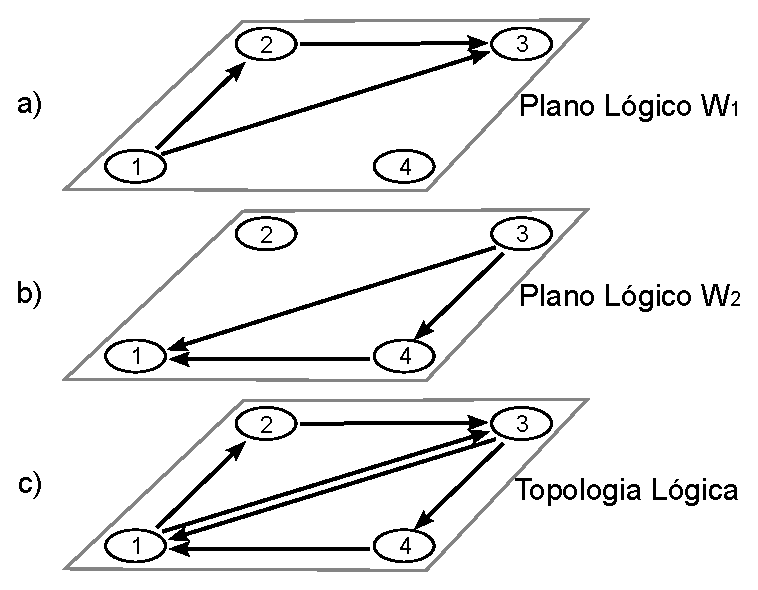
\includegraphics[bb=152 525 500 792,scale=0.7]{./figs/planos_logicos.eps}
	% planos_logicos.eps: 0x0 pixel, 300dpi, 0.00x0.00 cm, bb=152 524 442 792
	\caption{Esquema da separa��o da topologia l�gica por comprimento de onda.}
	\label{fig:planos_logicos}
\end{figure}

Essa forma de visualizar a topologia l�gica tem apenas a finalidade de facilitar a interpreta��o das restri��es,
pois permite ver o projeto como se fossem $W$ redes sem multiplexa��o sobrepostas.
Nas se��es que se seguem no restante deste cap�tulo, a separa��o da topologia l�gica por comprimento de onda ser� usada na explana��o sobre as restri��es do
modelo TWA.  

\subsection{Continuidade de Comprimentos de Onda e Capacidade}
\label{cap:twa-sec:Bconserv_Cap}

A Restri��o \ref{rest:DefCapFlow} acumula m�ltiplas fun��es, atuando como restri��o de continuidade de comprimentos de onda e limita��o de
capacidade. Em cada plano l�gico $w$, ela garante a continuidade das rotas f�sicas, onde os componentes topol�gicos devem formar uma caminho sobre a
topologia f�sica, conservando o mesmo comprimento de onda. Esses percursos n�o s�o controlados explicitamente; eles s�o garantidos pela conserva��o dos
componentes topol�gicos nos n�s intermedi�rios, semelhante a uma restri��o de conserva��o de fluxo \cite{ramamurthy99}. 

A Restri��o \ref{rest:DefCapFlow} � repetida na equa��o \ref{eq:DefCapFlow} para facilitar a leitura desta se��o. Nela, a conserva��o dos percursos l�gicos
� feita da seguinte forma: a soma dos componentes das liga��es l�gicas iniciadas em um n� $i$ no plano $w$, partindo de um n� intermedi�rio $v$, deve ser
menor ou igual � quantidade recebida. Isso � garantido se a equa��o \ref{eq:ConserB} for satisfeita.

\begin{equation}
\sum_{s} q_{sw}^{iv}\cdot A_s \leqslant Cap\cdot \left(\sum_{m} B_{iw}^{mv} - \sum_{n} B_{iw}^{vn}\right) \Forall{(i,v,w)} \mbox{, com $i\neq v$}
\label{eq:DefCapFlow}
\end{equation} 

\begin{equation}
   \sum_{n} B_{iw}^{vn} \leqslant \sum_{m} B_{iw}^{mv}  \Forall{(i,v,w)}
   \label{eq:ConserB}
\end{equation}

A equa��o \ref{eq:ConserB} pode ser reescrita na forma da equa��o \ref{eq:ConserBdif}, que define $LL^{iv}_w$, a diferen�a entre a soma dos
componentes chegando e saindo de $v$, originados em $i$ no plano $w$. O valor
$LL^{iv}_w$ representa a quantidade de liga��es l�gicas que n�o t�m continuidade ao passar por $v$, ou seja, s�o as liga��es l�gicas incidentes em $v$,
com origem em $i$ no plano $w$.

\begin{equation}
  LL^{iv}_w = \sum_{m} B_{iw}^{mv} - \sum_{n} B_{iw}^{vn} \geqslant 0 \Forall{(i,v,w)}
   \label{eq:ConserBdif}
\end{equation}

 Por sua vez, a equa��o \ref{eq:ConserBdif} � equivalente � equa��o
\ref{eq:ConserBcap}. Este �ltima � garantida pela Restri��o \ref{rest:DefCapFlow}, como fica demostrado pela equa��o \ref{eq:ConserBfim}, pois tomando-a
como premissa conclui-se a equa��o \ref{eq:ConserBcap}. Portanto, a equa��o \ref{eq:ConserB} � v�lida. 

\begin{equation}
   0  \leqslant Cap\cdot LL^{iv}_w \Forall{(i,v,w)}
   \label{eq:ConserBcap}
\end{equation}

\begin{equation}
   \sum_{s} q_{sw}^{iv}\cdot A_s  \leqslant Cap\cdot LL^{iv}_w \Forall{(i,v,w)}
   \label{eq:ConserBfim}
\end{equation}

Na figura \ref{fig:Bconserv} � ilustrada a forma como a conserva��o dos percursos l�gicos � feita. Nela v�-se dois componentes chegando no
n� intermedi�rio $v$, ambos comp�em liga��es l�gicas no plano $w$ iniciadas no n� $i$, que n�o est� representado na figura, igualmente ao componente que
deixa $v$. A soma dos valores dos componentes que chegam � $3$ e a dos que saem � $2$, portanto a conserva��o est� mantida. Neste exemplo, como h�
diferen�a de $1$ entre a quantidade de componentes chegando e saindo de $v$, ent�o, necessariamente h� $1$ liga��o l�gica terminando em $v$; para a qual
ele deixa de ser visto como um n� intermedi�rio, se tornando o destino dessa liga��o l�gica. A conserva��o n�o seria mantida no plano $w$ houvessem
componentes partindo de $v$ em maior quantidade do que chegando, pois ai n�o haveria rastreabilidade do percurso at� sua origem $i$. 
 
\begin{figure}[htb]
	\centering
	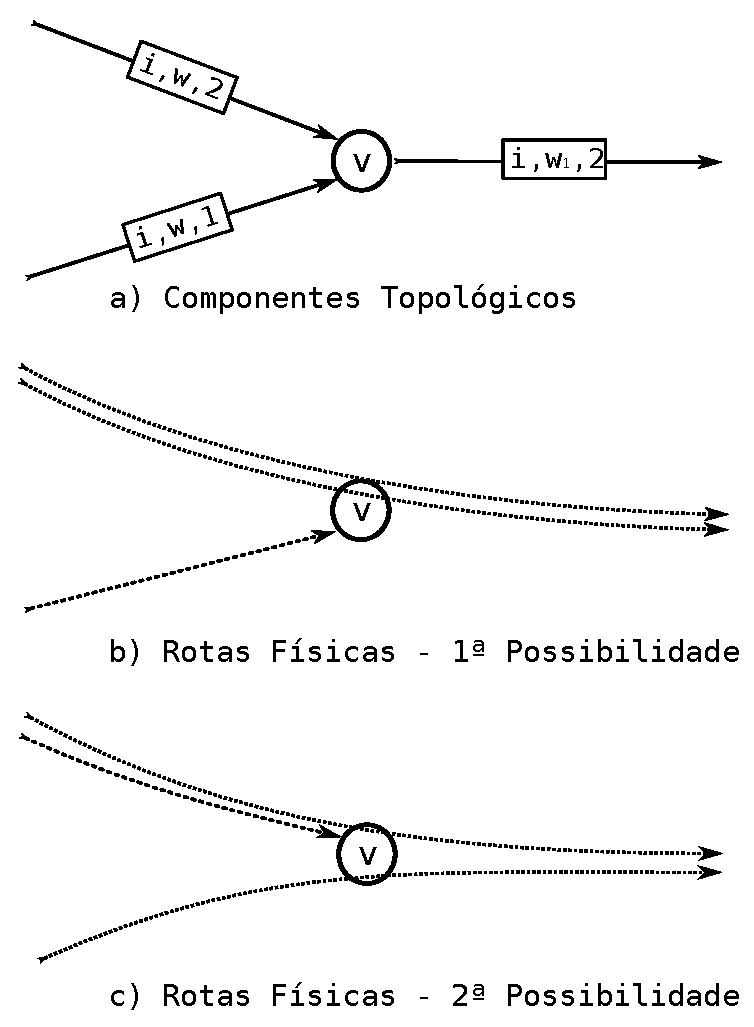
\includegraphics[bb=109 621 445 749,scale=0.7]{./figs/B_conserv.eps}
	% B_conserv.eps: 0x0 pixel, 300dpi, 0.00x0.00 cm, bb=106 272 452 749
	\caption{Conserva��o dos Percursos L�gicos.}
	\label{fig:Bconserv}
\end{figure}

A Restri��o \ref{rest:DefCapFlow} � um conjunto de equa��es, onde cada uma trata de um par $(i,j)$ em um plano l�gico $w$. Portanto, a capacidade das
liga��es l�gicas associadas ao par $(i,j)$ � a capacidade de cada uma ($Cap$) multiplicada pelo n�mero de liga��es l�gicas entre $(i,j)$ no plano l�gico
$w$.
Este segundo fator � $LL^{ij}_w$, calculado na equa��o \ref{eq:ConserBdif}. Todo o tr�fego passando pelas liga��es l�gicas $(i,j)$ nesse plano
deve ser limitado por $Cap\cdot
LL^{ij}_w$, o que de fato � feito pela Restri��o \ref{rest:DefCapFlow}. 

A Restri��o \ref{rest:DefCapFlow} ainda acumula uma fun��o que, por ser intuitiva, pode passar desapercebida, mas � fundamental para a consist�ncia do
modelo. Ela anula as fra��es de fluxo agregado entre os n�s n�o conectados diretamente por liga��es l�gicas. Quando $LL^{ij}_w = 0$, ou seja, n�o
h� liga��es l�gicas entre o par $(i,j)$ no plano $w$, as fra��es de fluxo $q_{sw}^{ij}$ ser�o anuladas pela Restri��o \ref{rest:DefCapFlow}, para todas as
origens $s$.

\subsection{Controle da Topologia F�sica}

Com a finalidade de controlar pela fun��o objetivo \ref{fo:MinC} a quantidade de liga��es f�sicas definidas pelos componentes topol�gicos, a Restri��o
\ref{rest:DefFis} acumula nas vari�veis $D_{mn}$ a multiplicidade determinada pelos componentes. Ela � repetida na
equa��o \ref{eq:DefFis} para facilitar a leitura desta se��o. Dado um par $(m,n)$, as equa��es
dessa restri��o s�o ainda separadas por comprimento de onda. Pois se todos os componentes topol�gicos alocados em $(m,n)$ usarem o mesmo $w$, apenas uma
liga��o f�sica ser� necess�ria. Se usarem comprimentos de onda diferentes, $D_{mn}$ precisar� atender ao maior desses componentes topol�gicos. Portanto, a
restri��o \ref{rest:DefFis}, minimiza a soma dos maiores de componentes topol�gicos em cada par $(m,n)$, por for�a do fator $CI$ na fun��o objetivo (Se��o
\ref{cap:twa-sec:funcaoobjetivo}).

\begin{equation}
\sum_i B_{iw}^{mn} \leqslant D_{mn} \Forall{(m,n,w)}
\label{eq:DefFis}
\end{equation} 

\begin{figure}[htb]
	\centering
	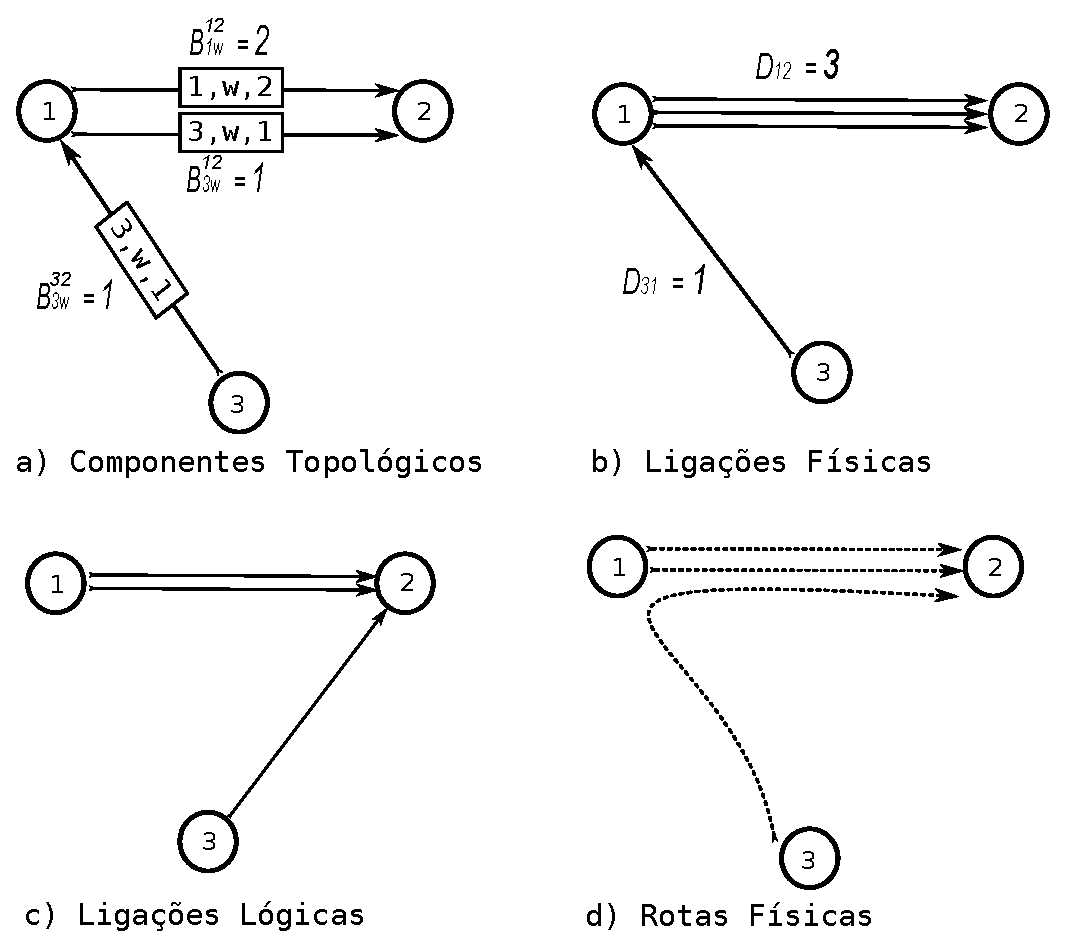
\includegraphics[bb=37 371 534 812, scale=0.7]{./figs/Var_Dmn.eps}
	% Var_Dmn.eps: 0x0 pixel, 300dpi, 0.00x0.00 cm, bb=34 593 536 800
	\caption{Interpreta��o dos componentes topol�gicos na vari�vel $D_{mn}$.}
	\label{fig:varDmn}
\end{figure}

Na Figura \ref{fig:varDmn} est� um exemplo de interpreta��o dos componentes topol�gicos na vari�vel $D_{mn}$. No item $a$ est�o os componentes topol�gicos
que definem as liga��es f�sicas indicadas no item $b$. Nos itens $c$ e $d$ est�o as liga��es l�gicas e as rotas f�sicas correspondentes.

\subsection{Conserva��o de Fluxo}

A conserva��o de fluxo � assegurada pelas Restri��es \ref{rest:ConservFlowOut} e \ref{rest:ConservFlow}, que tamb�m garantem o envio e a entrega das
demandas de tr�fego. Elas s�o repetidas nas equa��es \ref{eq:ConservFlowOut} e \ref{eq:ConservFlow} para facilitar a leitura desta se��o.  
Essas restri��es s�o semelhantes �s encontradas na modelagem agregada para o VTD \cite{ram02}. Al�m da separa��o do tr�fego por
comprimento de onda e da normaliza��o das vari�veis, como foi comentado na Se��o \ref{cap:twa-sec:VarFracFlow}, a interpreta��o das restri��es �
sutilmente diferente pois um par $(i,j)$ representa um conjunto de liga��es l�gicas. 

\begin{equation}
\sum_{jw} q_{vw}^{vj} = 1 \Forall{v} 
\label{eq:ConservFlowOut}
\end{equation} 
 
\begin{equation}
\sum_{iw} q_{sw}^{iv} - \sum_{jw} q_{sw}^{vj} = Q_{sv} \Forall{(s,v)} \mbox{, com $s\neq v$}
\label{eq:ConservFlow}
\end{equation}

Cada par $(i,j)$ � visto nas restri��es de controle de fluxo como um �nico caminho, unindo todos os planos l�gicos. Se o par representar na verdade
m�ltiplas
liga��es l�gicas, a diferen�a � que ele ter� uma capacidade maior de receber tr�fego, que � controlada pela Restri��o \ref{rest:DefCapFlow}. Deste modo,
essas restri��es funcionam da mesma forma que em \cite{ram96}. Portanto, s�o as restri��es de conserva��o de fluxo que fazem a correla��o ente os planos
l�gicos.

A Restri��o \ref{rest:ConservFlowOut} garante que todo o tr�fego originado em cada n� $v$ seja emitido para a rede, exigindo que a soma das fra��es
de tr�fego, em todos os planos l�gicos, que iniciam na origem ($i=s=v$) seja igual a $1$, ou seja, $100\%$ do tr�fego originado em $v$. 

Por sua vez, a
Restri��o \ref{rest:ConservFlow} garante que o tr�fego emitido seja encaminhado atrav�s da rede e entregue no destino. Fixada uma origem de tr�fego $s$,
para cada n� intermedi�rio $v$ ($v\neq s$) a por��o de tr�fego que deve ser entregue � $Q_{sv}$. Ela � igual � soma do tr�fego chegando por todos
os planos l�gicos $w$, vindo de qualquer n� intermedi�rio $i$, subtra�da da soma do tr�fego partindo com destino a qualquer n� $j$, em qualquer
plano $w$. O tr�fego n�o entregue em $v$ continua seguindo seu caminho pela rede at� seu destino, e deste modo � feita rastreabilidade do tr�fego at� sua
origem. Esta restri��o apenas n�o garante que o tr�fego seja emitido na origem, tarefa cumprida pela Restri��o \ref{rest:ConservFlowOut}.

O tr�fego pode ser subdividido e transportado simultaneamente por mais de uma liga��o l�gica entre o par $(i,j)$, no plano $w$. Neste caso, como as rotas
ter�o o mesmo comprimento de onda, eles n�o compartilham liga��es f�sicas ao longo do percurso. Mas essas rotas podem ainda n�o ser disjuntas, pois �
poss�vel compartilharem n�s intermedi�rios.

\section{Limita��es da Forma B�sica do TWA}

Dada a forma agregada como � feito o roteamento dos comprimentos de onda e tamb�m pela forma impl�cita do tratamento de m�ltiplas liga��es l�gicas, sem
separ�-las em vari�veis de decis�o pr�prias, algumas quest�es de menor complexidade n�o s�o decididas pelo TWA.  Na solu��o provida pelo modelo, s�o
alocados recursos suficiente para
atender ao projeto, da forma mais econ�mica poss�vel. Mas nem todos os detalhes da configura��o da rede s�o determinados.

Como ser� mostrado nesta se��o, essas omiss�es n�o
prejudicam o projeto dentro do escopo adotado. Podendo essas quest�es n�o resolvidas serem tratadas em fases posteriores do projeto a partir da solu��o
provida pelo modelo. Isso garante a simplicidade do TWA, permitindo uma modelagem com poucas restri��es e vari�veis. 

Na lista a seguir s�o enumeradas as limita��es da forma b�sica do TWA. Em seguida, cada uma ser� explicada e formas de trat�-las ser�o
sugeridas.

\begin{enumerate}
	\item Pode n�o haver uma forma �nica para configura��o das rotas f�sicas em cada plano l�gico.
	\item Podem ocorrer ciclos nas rotas f�sicas.
	\item Pode n�o ser poss�vel saber com exatid�o a dist�ncia percorrida pelo tr�fego.
	\item N�o � modelada a exata divis�o do tr�fego entre m�ltiplas liga��es l�gicas.
	\item N�o � poss�vel minimizar diretamente o congestionamento na forma b�sica do modelo.
	\item Podem haver liga��es f�sicas n�o utilizadas na solu��o.
\end{enumerate}

Como o roteamento de comprimento de onda � feito de forma agregada, podem haver mais de uma possibilidade de configura��o das rotas f�sicas em cada plano
l�gico. Na Figura \ref{fig:B_unsolved}, � mostrado um arranjo de componentes topol�gicos com duas possibilidades de interpreta��o. Necessariamente duas
liga��es l�gicas no plano $w_1$ passam transparentemente por $v_4$, enquanto uma nele termina. Ambas possibilidades de interpreta��o dos componentes s�o
v�lidas, ou seja, o TWA n�o modela o exato percurso f�sico das liga��es l�gicas em cada plano. Todavia,
isso n�o interfere na modelagem do restante do problema e n�o precisa ser resolvido nesta fase do projeto. 

De posse da solu��o provida pelo TWA, as
rotas que possu�rem alternativas de configura��o podem ser decididas levando-se em considera��o outras m�tricas n�o abordadas aqui, como por exemplo o fator
BL, que pondera tr�fego com a dist�ncia percorrida sobre a topologia f�sica \cite{Agrawal97}. Esse tratamento seria feito para cada par $(i,j)$
independente, sendo quest�es de baixa complexidade.

\begin{figure}[htb]
	\centering
	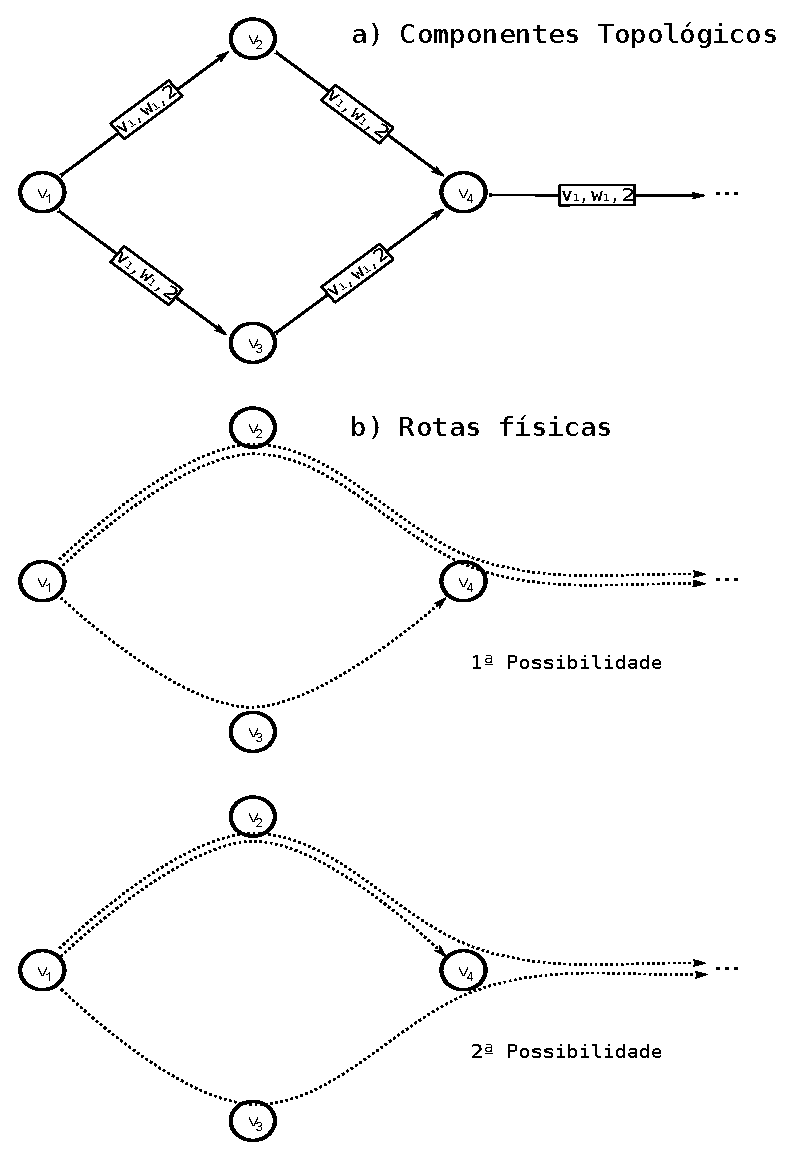
\includegraphics[bb=108 270 473 811,scale=0.7]{./figs/B_unsolved.eps}
	% B_unsolved.eps: 0x0 pixel, 300dpi, 0.00x0.00 cm, bb=108 270 473 811
	\caption{Duas possibilidades de interpreta��o dos componentes topol�gicos.}
	\label{fig:B_unsolved}
\end{figure}

Na forma b�sica do modelo TWA, podem aparecer ciclos nas rotas f�sicas, pois n�o h� esse controle no modelo b�sico. Isso poderia ser minimizado adicionando
a soma de todos os componentes topol�gicos na fun��o objetivo. Mas esses ciclos n�o interferem na modelagem e podem ser facilmente localizados e retirados
analisando a solu��o obtida.

Outra quest�o a ser determinada envolve o fato de um par $(i,j)$ poder representar m�ltiplas liga��es l�gicas. Sempre haver� banda suficiente
para atender ao tr�fego alocado respeitando � capacidade individual; isso � garantido pela Restri��o \ref{rest:DefCapFlow}. Todavia, na distribui��o do
tr�fego cada par $(i,j)$ � visto como um �nico caminho, e o tr�fego � separado apenas por comprimento de onda. O tr�fego pode ser subdividido e
transportado simultaneamente por mais de uma liga��o l�gica entre o par $(i,j)$ no plano $w$, sem compartilhar liga��es f�sicas ao longo do percurso. Mas
n�o fica definida a divis�o de tr�fego entre cada liga��o. 

A exata divis�o do tr�fego tamb�m pode ser definida em outra fase do projeto
e n�o precisa ser modelada aqui. Todavia, seria razo�vel assumir que o tr�fego fosse dividido igualmente entre as liga��es, para n�o sobrecarregar uma em
detrimento da outra. Ou poderia-se tamb�m aplicar o fator BL para fazer a divis�o do tr�fego considerando a dist�ncia percorrida. Novamente, essas
situa��es s�o pontuais, resolvendo-se para cada par $(i,j)$ individualmente sem demandar expressivo custo computacional.

Em virtude de n�o ser modelada a exata divis�o do tr�fego entre m�ltiplas liga��es l�gicas, n�o � poss�vel minimizar diretamente o
congestionamento \cite{ram02}. Mas, a capacidade das liga��es l�gicas pode exercer o papel de limitante superior (\textit{upper bound}) para o
congestionamento. Conjuntamente com a minimiza��o do tr�fego na fun��o objetivo, como foi comentado na Se��o \ref{cap:twa-sec:funcaoobjetivo}, temos uma boa
abordagem para tratar do congestionamento, como foi demostrado em \cite{Renato06}.

Por fim resta tratar da possibilidade da topologia f�sica determinada pelos componentes topol�gicos poder ser superestimada na vari�vel $D_{mn}$.
A Restri��o \ref{rest:DefFis} apenas exige que a vari�vel $D_{mn}$ seja suficiente para atender aos componentes topol�gicos, mas permite que ela assuma
valores maiores que o necess�rio. Todavia, esse poss�vel excesso n�o interfere na consist�ncia do que � modelado pelos componentes topol�gicos. Al�m disso,
ele � controlado indiretamente minimizando a fun��o objetivo, por meio do custo de instala��o, e pode ainda ser tratado analisando a solu��o fornecida,
extraindo os valores corretos diretamente dos componentes topol�gicos. A corre��o feita atrav�s da fun��o objetivo funcionaria tamb�m com qualquer outra
m�trica diretamente relacionada com a vari�vel $D_{mn}$ que fosse minimizada. 









%%%%%%%%%%%%%%%%%%%%%%%%%%%%%%%%%%%%%
%% Metodologia Proposta
%% Copyright 2009 Marcelo de Oliveira Lima.
%% Este documento � distribu�do nos termos da licen�a 
%% GNU General Public License v2.
%%%%%%%%%%%%%%%%%%%%%%%%%%%%%%%%%%%%%


\chapter{Projeto Completo de Redes �pticas em Hierarquia}
\label{metodo}
\thispagestyle{empty}

O tipo de topologia para redes �pticas com roteamento por comprimento de onda mais estudado na literatura � a topologia em malha. No entanto, existem trabalhos
que exploram redes com arquitetura em hierarquia, mais precisamente an�is em hierarquia \cite{fonseka}, \cite{spie06}, \cite{conftele07}. Contudo, at� onde
possu�mos conhecimento, a jun��o destes dois tipos de arquiteturas ainda n�o foi explorado no contexto de WRONs. Neste trabalho, decidiu-se por estudar uma
arquitetura de malhas em hierarquia, onde existe uma sub-rede na hierarquia superior que ser� chamada de \textit{backbone}, cujos seus n�s pertencem cada um a
uma outra sub-rede de hierarquia inferior. Cada sub-rede inferior � chamada de \textit{cluster}. Estas sub-redes podem assumir arquiteturas em malha
ou anel, de acordo com o grau l�gico em estudo. Quando se trabalha com grau l�gico 1, trata-se de um anel, caso contr�rio de uma topologia em malha. A figura
\ref{fig:hierarquia} ilustra uma topologia hier�rquica gen�rica. 

\begin{figure}[htb!]
 \begin{center}
 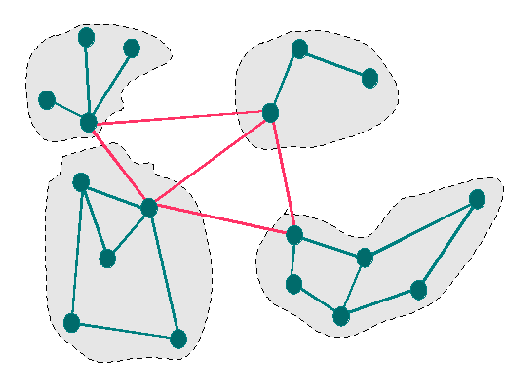
\includegraphics[scale=1.1]{./figs/hierarquica.eps}
 % hierarquica.eps: 0x0 pixel, 300dpi, 0.00x0.00 cm, bb=0 0 238 170
 \caption{Exemplo de topologia de rede em hierarquia.}
 \label{fig:hierarquia}
 \end{center}
\end{figure}


O objetivo principal deste trabalho � criar uma metodologia que viabilize o projeto completo de malhas hier�rquicas, aproveitando o potencial da
modelagem TWA, juntamente com m�todos heur�sticos. Tomando como requisitos apenas um conjunto de n�s de rede, com sua disposi��o geogr�fica e requisi��es de
tr�fego esperadas. O projeto completo abrange aqui, al�m das vari�veis de decis�o suportadas pelo modelo TWA, a escolha da estrutura hier�rquica da rede.

Idealmente, o projeto completo de uma malha hier�rquica poderia ser feito incluindo restri��es no TWA que modelassem a hierarquia, semelhante ao que foi
feito em \cite{tesetommy}. Todavia, com o objetivo de tratar do projeto de redes de grande porte, optamos por uma abordagem simplificada em termos de modelagem
matem�tica, deixando a escolha da composi��o das sub-redes a cargo de uma heur�stica desenvolvida a partir de algoritmos gen�ticos. Conforme mencionado, as
hierarquias projetadas neste trabalho ter�o apenas dois n�veis, com um \textit{backbone} central e \textit{clusters} perif�ricos, de forma semelhante aos
exemplos encontrados na literatura para an�is hier�rquicos.

Uma simplifica��o adotada � que as liga��es entre os \textit{clusters} e o \textit{backbone} ser�o opacas, ou seja, todos os componentes de uma liga��o l�gica
est�o em um mesmo n�vel da hierarquia. Deste modo, o \textit{backbone} e os \textit{clusters} podem ser vistos como redes independentes, exceto pelo tr�fego que
cruza de um n�vel hier�rquico para outro, chamado de tr�fego de acesso. Este tr�fego pode ser acumulado nos n�s de acesso ao \textit{backbone} (como
ser� mostrado na Se��o \ref{sec:fitness}), de modo que sua distribui��o e roteamento podem ser feitos paralelamente em cada sub-rede.

Assim, para definir a estrutura hier�rquica basta separar os n�s da rede em conjuntos, que formar�o cada \textit{cluster}, e escolher em cada um qual ser�
o n� de acesso ao \textit{backbone}. Por sua vez, este �ltimo ser� formado pelo conjunto de n�s de acesso, tamb�m chamados de super-n�s \cite{spie06},
\cite{conftele07}.

Dessas considera��es, temos que cada sub-rede pode ser projetada separadamente, eliminando a necessidade de uma modelagem para toda a hierarquia.

A escolha da estrutura hier�rquica, como ser� definida, � um Problema de Cobertura de Conjuntos (PCC), com uma fun��o objetivo especial. A formula��o
cl�ssica
do PCC � um problema de programa��o linear inteira NP-completo \cite{cormen02}. Portanto, abordagens heur�sticas s�o adequadas para sua resolu��o. Neste
trabalho utilizamos um algoritmo gen�tico nesta etapa.
  
Tendo sido determinada a estrutura hier�rquica, cada sub-rede � modelada com o TWA. Nesta fase, a estrat�gia adotada foi definir par�metros de qualidade
satisfat�rios para as vari�veis de interesse, de modo que qualquer solu��o vi�vel encontrada j� seria suficiente para garantir a qualidade do projeto.

As vari�veis de interesse em quest�o s�o o congestionamento da rede, o total do tr�fego retransmitido, o custo de instala��o da rede f�sica, o n�mero de
comprimentos de onda utilizados e o n�mero total de transceptores utilizados. As duas primeiras s�o comumente tratadas pela literatura no projeto de topologias
l�gicas (VTD), sem considerar o projeto da rede f�sica ou o roteamento e aloca��o de comprimentos de onda (RWA) \cite{ram02}.

Para estabelecer par�metros de qualidade para congestionamento e tr�fego retransmitido, s�o estimados estatisticamente as m�dias e desvios padr�es de suas
popula��es de solu��es vi�veis para o VTD, em cada sub-rede. Nessas infer�ncias � garantida a representatividade das amostras obtidas, como ser� mostrado na
se��o \ref{sec:subredes:estatisticas}.

Para o n�mero de comprimentos de onda, foi utilizada uma estrat�gia adotada anteriormente em \cite{SBPO2009}. Tentamos obter solu��es com um comprimento
de onda apenas e vamos incrementando esse n�mero enquanto n�o for poss�vel encontrar solu��es vi�veis. Essa t�cnica deriva de uma caracter�stica do TWA, pois o
n�mero de vari�veis no modelo � m�ltiplo do n�mero de comprimentos de onda adotado.
%O que torna vi�vel essa investiga��o partindo dos menores n�meros de comprimentos de onda. 

Por sua vez, o custo de instala��o da rede f�sica � controlado garantindo que seja menor, proporcionalmente, que o custo de uma rede real bem conhecida, a
NSFNET \cite{ram02}. A forma como � estabelecida essa proporcionalidade ser� descrita na se��o \ref{sec:subredes:custo_fisico}. Estamos considerando como
custo de instala��o apenas a dist�ncia entre os n�s da rede, que representa o comprimento dos enlaces de fibra instaladas entre os mesmos. O dimensionamento dos
n�s poder� ser feito com base no projeto obtido desta metodologia, que dever� demandar o m�nimo poss�vel de recursos da rede.

No projeto de topologias l�gicas, o n�mero de transceptores da rede normalmente define as inst�ncias do problema \cite{ram02}, pois est� relacionado com o
dimensionamento dos n�s da rede. Essa abordagem tamb�m foi utilizada aqui, todavia, na literatura � comum definir o n�mero exato de transceptores que cada
inst�ncia possui, pelo produto entre grau l�gico e o n�mero de n�s da rede, com n�veis diferentes de limita��o de tr�fego para cada uma \cite{Sivarajan01}.
Neste trabalho, n�s apenas limitamos o n�mero de transceptores, permitindo que o modelo encontre solu��es mais econ�micas para este par�metro.

As pr�ximas se��es s�o dedicadas a explica��o detalhada dos principais aspectos que comp�em as etapas da metodologia proposta. Uma vis�o geral do procedimento
est� apresentada na figura\ref{fig:descr.proc}. Existem tr�s etapas sequenciais.


\begin{figure}[!htb]
\begin{center}
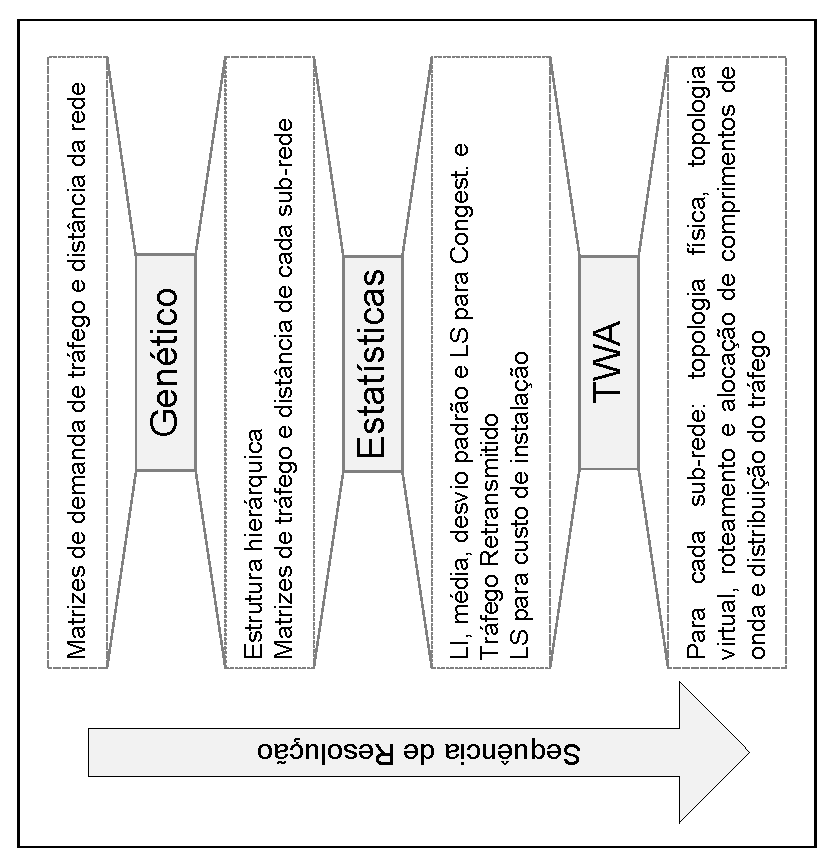
\includegraphics[scale=0.9, angle=270]{./figs/metodologia.eps}
% descr.proc.eps: 595x842 pixel, 72dpi, 20.99x29.70 cm, bb=
\caption{Resumo da metodologia de projeto.}
\label{fig:descr.proc}
\end{center}
\end{figure}


Na primeira etapa, s�o fornecidos como dados as matrizes de demandas de tr�fego e dist�ncias, �nicos dados de entrada do projeto. Um algoritmo
gen�tico faz a separa��o dos n�s em sub-redes. Sua fun��o objetivo minimiza o tr�fego transferido entre as sub-redes e a dist�ncia entre os
n�s, ou seja, procura-se concentrar o tr�fego no interior das sub-redes, e form�-las com n�s geograficamente pr�ximos. Um resultado secund�rio dessa fase
s�o as matrizes de dist�ncia e tr�fego para cada sub-rede.

Na fase intermedi�ria, s�o obtidos os limites superiores (\textit{upper bounds} - UB) para o congestionamento e o tr�fego retransmitido na rede, por meio de
infer�ncia estat�stica baseada na m�dia e desvio padr�o dos resultados das avalia��es de amostras de solu��es vi�veis para o VTD. Estes limites superiores s�o
valores m�ximos admiss�veis para o congestionamento e o tr�fego retransmitido, impostos �s vari�veis do modelo de programa��o inteira-mista para garantir, com
rela��o a estas m�tricas, a qualidade da solu��o a ser obtida na pr�xima etapa . Al�m dos UB, para validar os resultados, s�o tamb�m calculados limites
inferiores te�ricos (\textit{lower bounds} - LB) para essas m�tricas. As formula��es para os LB foram apresentadas por \cite{dissertFabio}, e os UB s�o
calculados a partir da m�dia e do desvio padr�o. Por fim, tamb�m s�o calculados UB para o custo de instala��o f�sica de cada sub-rede.

A �ltima etapa consiste na resolu��o do modelo TWA para cada sub-rede, respeitando os \textit{bounds} (UB e LB) calculados e visando utilizar o menor n�mero
poss�vel de comprimentos de onda. O resultado desta �ltima fase fornece a solu��o do projeto, representado pelas topologias f�sica e l�gica, bem como a forma de
roteamento e aloca��o dos comprimentos de onda, em fun��o da da distribui��o das demandas de tr�fego esperadas. Esses resultados s�o referentes �s sub-redes em
separado, por�m, quando s�o agrupados, representam o resultado global para uma WRON com topologias hier�rquicas.


\section{Estrutura Hier�rquica}
\label{sec:EstruturaHierarquica}

%%%%% Reda��o antiga %%%%%%%%%%%%%%%
% A quantidade e o tamanho dos 
% \textit{clusters} � livre, sendo definido apenas um mesmo n�mero $M_i$ para o m�nimo de \textit{clusters} e o seu tamanho m�nimo. Deste modo, se
% a rede possui $n$ n�s, ent�o o n�mero m�ximo de \textit{clusters} e seu tamanho m�ximo ($M_a$) ser� igual a $\lfloor n/M_i \rfloor$.

A quantidade e o tamanho dos \textit{clusters} � livre, sendo definidos um tamanho m�ximo $M_a$ e um m�nimo $M_i$, al�m da quantidade m�xima de
clusters $Q_a$. Uma quantidade m�nima de \textit{clusters} fica implicitamente definida por esses valores, n�o sendo necess�rio control�-la.
 Assim, uma rede de $n$ n�s e $k$ \textit{clusters}, � representada por dois vetores. Um vetor de tamanho $k$ contendo os tamanhos dos \textit{clusters}
($T=(t_1,\cdots,t_k)$) e outro
de tamanho $n$ contendo uma permuta��o dos n�s da rede ($P=(p_1,\cdots,p_n)$). Onde o primeiro \textit{cluster} � representado por $(p_1,\cdots,p_{t_1})$, o
segundo por $(p_{[1+\,t_1]},\cdots,p_{[t_1+\,t_2]})$, e o $i$-�simo \textit{cluster} � representado por:

$$(p_{[1+\,s_{(i\,-1)}]},\cdots,p_{[s_{i}]})\mbox{, onde } s_i=t_1 + t_2 + \cdots + t_i$$

Em cada \textit{cluster}, o primeiro n� da sequ�ncia � interpretado como o n� de acesso ao \textit{backbone}. Portanto, o \textit{backbone} � representado
por:

$$(p_1,p_{[1+\,t_1]},\cdots,p_{[1+\,s_{(k\,-1)}]})$$

Para a escolha da estrutura hier�rquica da rede foi implementado um algoritmo gen�tico com a biblioteca {\itshape Galib} (Ap�ndices \ref{ga} e
\ref{galib}). Para representar a hierarquia, � definido um cromossomo utilizando um vetor de tamanho $n+Q_a$, contendo uma
permuta��o dos n�meros inteiros positivos at� esse valor: $n$ n�meros para representar os n�s da rede mais $Q_a$ n�meros, candidatos a tamanho de
\textit{cluster}. 
A interpreta��o do cromossomo como uma hierarquia � feita da seguinte forma: 

\begin{enumerate}
\item Separa-se o cromossomo em dois vetores, mantendo-se a ordem dos n�meros. O primeiro, de tamanho $n$, cont�m os n�meros menores ou iguais � $n$. Este
� o vetor $P$, uma permuta��o dos n�s da rede. O segundo vetor ($C=(c_1,\cdots,c_{Q_a})$) cont�m os n�meros maiores que $n$ e dar� origem ao vetor de
tamanhos
$T$. 
\item A partir de $c_1$, iterativamente, faz-se $t_i= M_i + [c_i\mod\Delta]$, enquanto $n - s_i \geqslant M_i$, onde $\Delta = (M_a - M_i)$ e $s_i$ como
definido acima. Ou seja, enquanto o n�mero de n�s
restante n�o for menor que o m�nimo admitido para formar outro \textit{cluster}. Quando isso ocorrer, descarta-se o valor calculado para $t_i$ e forma-se o
�ltimo \textit{cluster} com os n�s restantes. 
\end{enumerate}

Note que o c�lculo de $t_i$, como foi definido acima, leva o valor de $c_i$ para um intervalo de poss�veis tamanhos de \textit{clusters}. Os valores que
dar�o origem ao vetor de tamanhos $T$, foram definidos como n�meros maiores que $n$ para simplificar a codifica��o do cromossomo. Sendo este uma simples
permuta��o de inteiros entre $1$ e $n+Q_a$, sem uma estrutura particular, permitiu utilizar operadores gen�ticos pr� dispon�veis na biblioteca
\textit{Galib} e bem conhecidos na literatura \cite{ga2}. S�o eles os operadores gen�ticos do c�digo $Ex26$ da \textit{Galib}, com a
fun��o de cruzamento: \textit{Edge Recombination Crossover}. 

A estrutura de cromossomo utilizada n�o permite ao algoritmo gen�tico visitar todas as poss�veis configura��es da hierarquia, da forma como foi definido na
in�cio desta se��o. Dentre as limita��es, destaca-se o fato do desenho do cromossomo inibir a cria��o de hierarquias com \textit{clusters}
de tamanho uniforme. Pois os tamanhos s�o retirados de uma permuta��o dos n�meros de $n+1$ at� $n+Q_a$, m�dulo $\Delta$; isso dificulta ocorrer
entradas repetidas no vetor de tamanhos. Al�m disso, deve-se garantir que a soma de tamanhos poss�veis cobre $n$, o que pode n�o ocorrer dependendo dos
valores de $M_a$, $M_i$ e $Q_a$. Isso � garantido se a inequa��o a seguir for verdadadeira:

$$ n \leqslant \sum_{i=1}^{Q_a} M_i + [(n + i)\mod\Delta] $$ 

Essas desvantagens no modelo do cromossomo s�o compensadas, pelo fato dos operadores gen�ticos utilizados suportarem indiv�duos formados por permuta��o de
n�meros inteiros, sem gerar solu��es invi�veis. Isso contribui para a efici�ncia do algoritmo \cite{ga1}, pois evita visitar solu��es que n�o contribuem
para a melhora na evolu��o. Al�m disso, economizou-se o esfor�o em seu desenvolvimento, implementa��o e valida��o.

O algoritmo gen�tico adotado foi o \textit{GADemeGA}, tamb�m dispon�vel na \textit{Galib}, que mant�m popula��es paralelas com probabilidade de migra��o
a cada gera��o da evolu��o. Os par�metros de configura��o das fun��es da \textit{Galib} foram mantidos em seus valores padr�o e demostraram desempenho
satisfat�rio, mas para implementa��es mais robustas � recomendado que sua calibragem seja melhor estudada.


\section{Qualidade da Estrutura Hier�rquica}
\label{sec:fitness}

Al�m da codifica��o do cromossomo e da escolha das fun��es da \textit{Galib} a serem utilizadas, o algoritmo gen�tico se completa com a defini��o da sua
fun��o objetivo, que atribuir� uma m�trica de qualidade para os cromossomos. 

Dois par�metros importantes no projeto de uma rede s�o os custos de instala��o e opera��o da mesma \cite{bannister90}, \cite{liu2008}, \cite{guan}. Na separa��o
dos conjuntos de n�s que formar�o as sub-redes um fator que influencia fortemente no custo de instala��o � a dist�ncia entre os n�s. Se as sub-redes forem
agrupados de modo que n�s pr�ximos fa�am parte do mesmo conjunto, haver� uma tend�ncia de menor custo de instala��o dos enlaces. Por esse motivo, a dist�ncia
m�dia entre os n�s � uma boa m�trica para minimizar o custo de instala��o f�sico.

N�o obstante, se dois n�s que possuem grande quantidade de demanda de tr�fego entre eles estiverem no mesmo \textit{cluster}, eles deixar�o de rotear pelo
\textit{backbone} esse forte fluxo. Se essa tend�ncia se mantiver por toda a rede, com as maiores demandas representando tr�fego dom�stico dos
\textit{clusters}, � razo�vel supor que esta configura��o poupar� custo de opera��o da rede, pois estar� reduzindo o tr�fego de acesso ao \textit{backbone} e
tamb�m o retransmitido entre n�s intermedi�rios. Definimos tr�fego de acesso como sendo todo aquele que cruza as hierarquias da rede, em ambos os sentidos, ou
seja, se origina em uma sub-rede com destino a outra. Destaca-se que para efeito de resultados do projeto, ele � computado apenas nos super-n�s que fazem a sua
interface entre hierarquias distintas, pois nos demais n�s ele � contabilizado indistintamente como tr�fego retransmitido.

A figura \ref{fig:ga.group} ilustra o processo de decis�o do gen�tico, onde ele busca agrupar os n�s fisicamente mais pr�ximos e ao mesmo tempo
seleciona em cada grupo, ou sub-rede, um n� que ser� utilizado como interface entre as demais sub-redes, de forma a minimizar o tr�fego de acesso. Esses n�s de
acesso est�o destacados no interior de cada sub-rede. 


\begin{figure}[!htb]
\begin{center}
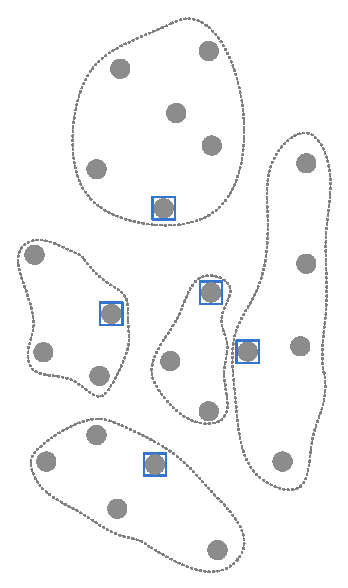
\includegraphics[scale=1.3, angle=270]{./figs/ga_group.eps}
\caption{Ilustra��o do processo de decis�o do gen�tico.}
\label{fig:ga.group}
\end{center}
\end{figure}


Deste modo, a fun��o objetivo do algoritmo gen�tico foi definida como a soma da dist�ncia m�dia entre os n�s da hierarquia ($M$) com o total de tr�fego
de acesso ao \textit{backbone} ($T$). Esses valores podem ser calculados sem que seja necess�rio conhecer a estrutura completa da rede, basta sabermos a
estrutura hier�rquica, como foi definida na se��o anterior.

Como resultado do algoritmo gen�tico, al�m da estrutura hier�rquica da rede, tamb�m s�o derivadas as matrizes de demanda e dist�ncia de cada sub-rede. As
matrizes de dist�ncias s�o apenas um subconjunto da original. Enquanto que as matrizes de demanda acumulam nos n�s de acesso todo tr�fego que dever� entrar no
\textit{cluster} e sair dele.

A equa��o \ref{DefDistMed} define a f�rmula de c�lculo para $M$. Primeiro calcula-se a soma das dist�ncias entre os n�s de cada grupo, \textit{backbone}
($TDist_{bk}$) e \textit{clusters} ($TDist_{cl}$), e a m�dia desses valores � tomada como a dist�ncia m�dia da hierarquia. Dependendo do estudo de caso em
quest�o, pode ser de interesse ponderar esses termos, possivelmente atribuindo maior peso �s dist�ncias do \textit{backbone}. Na equa��o \ref{DefDistMed} esses
pesos ($PesoDist_{bk}$ e $PesoDist_{cl}$) est�o apresentados multiplicando seus respectivos termos de dist�ncia. O denominador no c�lculo de $M$
� a soma da quantidade de termos contidos nas matrizes de dist�ncias do \textit{backbone} ($NumDist_{bk}$) e dos \textit{clusters} ($NumDist_{cl}$).

\begin{equation}
M = \frac{TDist_{bk}\cdot PesoDist_{bk} + TDist_{cl}\cdot PesoDist_{cl}}{NumDist_{bk} + NumDist_{cl}}
\label{DefDistMed}
\end{equation} 

Para calcular o tr�fego de acesso em um super-n�, soma-se todo o tr�fego originado dentro do seu \textit{cluster} cujo destino s�o n�s de outros
\textit{clusters}, mais o tr�fego da condi��o inversa. Ou seja, que origina-se em outros \textit{clusters} e possui destino no interior do \textit{cluster} a
que pertence o referido super-n�. Acumulando-se essa soma para todos os super-n�s, temos o total de tr�fego de acesso da rede $T$.

A equa��o \ref{DefTrafAcesso} mostra que o total de tr�fego de acesso tamb�m pode ser ponderado ($PesoTrafAcesso$) de acordo com o interesse do estudo
realizado.

\begin{equation}
T = TrafAcesso\cdot PesoTrafAcesso
\label{DefTrafAcesso}
\end{equation} 

Nos experimentos que ser�o apresentados no pr�ximo cap�tulo, as entradas das matrizes de demanda de tr�fego e dist�ncia possuem a mesma ordem de grandeza.
Podendo representar respectivamente a taxa de transfer�ncia de pacotes em $Gbits/s$ e centenas de quil�metros de dist�ncia por exemplo. Fica claro que neste
caso $M$, por ser uma m�dia, tem ordem de grandeza bem inferior � de $T$, que � uma soma simples. Portanto, para garantir o equil�brio entre as duas
m�tricas, um teste piloto deve ser feito para estabelecer uma propor��o que deixe $M$ e $T$ com a mesma ordem de grandeza. Feito isso, tamb�m � poss�vel
atribuir pesos para cada um, conforme for o interesse do estudo de caso em quest�o. A equa��o \ref{DefFitness} ilustra a f�rmula de c�lculo da fun��o objetivo
do gen�tico (\textit{fitness}), ilustrando o uso de um fator de calibragem ($C_a$) a fim de tornar $M$ e $T$ compat�veis em termos de ordem de grandeza.

\begin{equation}
Fitness = M\cdot C_a + T
\label{DefFitness}
\end{equation} 

O crit�rio de parada adotado para o algoritmo gen�tico foi a converg�ncia da fun��o objetivo, baseada na estagna��o da fun��o objetivo. Quando deixar de
haver melhora na evolu��o por um dado n�mero de gera��es, o algoritmo gen�tico � interrompido. A efici�ncia deste crit�rio tamb�m ser� analisada quando
forem feitos experimentos computacionais. 


\section{Qualidade do Projeto das Sub-Redes}
\label{sec:subredes}

Para cada sub-rede, s�o definidos conjuntos de par�metros de qualidade para o seu projeto. Esses par�metros devem ser considerados satisfat�rios para cada
inst�ncia, representando uma qualidade elevada para a rede, pois na �ltima etapa do procedimento eles ser�o fornecidos para o modelo TWA a fim de se obter uma
solu��o vi�vel que atenda a todos esses par�metros.

Distinguindo as inst�ncias pelo grau l�gico, para o congestionamento nas sub-redes e o total de tr�fego retransmitido nas mesmas, s�o analisadas
estatisticamente as popula��es de solu��es para o VTD. Pois essas s�o m�tricas comumente tratadas nesse problema \cite{ram02}. Dessa an�lise, ser�o
estabelecidas as limita��es para o congestionamento e para o tr�fego retransmitido. Al�m disso, tamb�m ser� definida uma limita��o para o custo de instala��o da
rede f�sica, que � independente da inst�ncia.

Na se��o \ref{sec:subredes:estatisticas} ser� explicado o processo de estima��o das estat�sticas para congestionamento e tr�fego retransmitido. O crit�rio de
limita��o do custo de instala��o est� descrito na se��o \ref{sec:subredes:custo_fisico}. Por fim, para que as limita��es das m�tricas possam ser repassadas ao
modelo TWA ser�o necess�rias restri��es adicionais, sendo estas apresentadas na se��o \ref{sec:subredes:restricoes}.


\subsection{Congestionamento e Tr�fego Retransmitido}
\label{sec:subredes:estatisticas}

Conforme os trabalhos que tratam do VTD, as inst�ncias s�o determinadas pelo n�mero total de transceptores utilizados, que � uma fun��o do grau l�gico da
rede. Pois o n�mero total de transceptores utilizados � dado justamente pelo n�mero de n�s da rede multiplicado pelo seu grau l�gico \cite{ram02}. 

Deste modo, para cada grau l�gico geramos aleatoriamente uma amostra de solu��es para a topologia l�gica da rede. Modelos de programa��o linear foram
implementados em \textit{AMPL} \cite{ampl} para distribuir o tr�fego da rede sobre cada topologia l�gica, atrav�s do solver \textit{GLPK} (\textit{GNU
Linear Programming Kit} - gnu.org/software/glpk). Obtendo, para cada topologia l�gica gerada, a distribui��o de tr�fego �tima para o congestionamento da
rede e tamb�m para o total do tr�fego retransmitido \cite{Renato06}.

Dessas amostras estimamos a m�dia e o desvio padr�o das popula��es para o congestionamento e para o tr�fego retransmitido, garantindo a representatividade de
cada amostra. Esta estima��o se classifica como um problema de Estat�stica Indutiva \cite{estatistica}, que tem como objetivo tirar conclus�es probabil�sticas
sobre aspectos das popula��es, com base na observa��o de amostras extra�das das mesmas. Estas amostras servem de base para infer�ncias que s�o feitas a cerca
das respectivas popula��es. Para tanto, sup�e-se que os valores da popula��o se distribuem segundo um dado modelo de distribu��o de probabilidade cujos
par�metros necessitam ser estimados. Segundo \cite{estatistica}, esta suposi��o � plaus�vel, pois, em muitos casos, pode-se antecipar com razo�vel precis�o, um
modelo para a distribui��o da popula��o. O processo de estima��o de par�metros utilizado � denominado de estima��o por intervalo, onde � contru�do um intervalo,
o qual deve, com probabilidade conhecida, conter o par�metro.

Chamamos de estimador a quantidade, calculada em fun��o dos elementos da amostra, que ser� usada no processo de estima��o do par�metro desejado. O estimador �
uma estat�stica e ser�, portanto, uma vari�vel aleat�ria caracterizada por uma distribui��o de probabilidade e seus respectivos par�metros pr�prios. E
chamaremos de estimativa cada particular valor assumido por um estimador.

Ao intervalo que, com probabilidade conhecida, dever� conter o valor real do par�metro chamaremos intervalo de confian�a para esse par�metro. � probabilidade,
que ser� designada por $1 - \alpha$, de que um intervalo de confian�a contenha o valor do par�metro chamaremos grau de confian�a do respectivo intervalo. Dessa
forma, vemos que $\alpha$ ser� a probabilidade de erro na estima��o por intervalo, isto �, a probabilidade de errarmos ao afirmar que o valor do par�metro est�
contido no intervalo de confian�a. Ser� suposto que os intervalos de confian�a s�o sim�tricos em probabilidade, isto �, a probabilidade do par�metro ficar fora
do intervalo � sua esquerda � igual � probabilidade de ficar fora � direita, ambas iguais a $\alpha/2$. A partir do exposto, pode-se afirmar que o
  intervalo conter� ou n�o o par�metro, com probabilidade $1 - \alpha$ e $\alpha$, respectivamente.

Para determinar o tamanho necess�rio de cada amostra, de modo que estas sejam representativas para cada par�metro estat�stico estimado, utilizamos o m�todo
interativo apontado por \cite{estatistica}. Para a m�dia, o intervalo de confian�a pode ser obtido por:

$$e_0 = Z_{\alpha/2}\cdot \frac{\sigma}{\sqrt{n}}$$

Onde $e = 2 \cdot e_0$ � a margem de erro, a amplitude de intervalo de confian�a, $Z_p$ � a distribui��o normal reduzida, $1 - \alpha$ � o n�vel de confian�a
exigido, $\sigma$ � o desvio padr�o populacional e $n$ � o tamanho da amostra. Mas ao inv�s de estimar o intervalo de confian�a, desejamos, a partir de uma
margem de erro e n�vel de confian�a desejados, estimar o tamanho de amostra necess�rio. Resolvendo a equa��o acima para $n$, temos:

$$n = \left( \frac{Z_{\alpha/2}\cdot \sigma}{e_0} \right)^2 $$

Onde $n$ agora � a estimativa para o tamanho da amostra. Embora n�o conhe�amos o desvio padr�o populacional $\sigma$, a rela��o a seguir permite a
substitui��o pela sua estimativa amostral $s$:

%$$s = \sqrt{\frac{\sum_{i=1}^{n} (X_i - \bar X)^2}{n-1}}$$

$$ t_{(n - 1, \alpha/2)} \cdot s = Z_{\alpha/2}\cdot \sigma $$

Onde $t_{(n - 1, p)}$ � a distribui��o $t$ de \textit{Student} com $n - 1$ graus de liberdade, que faz compensar o efeito da maior incerteza embutida pelo
uso se $s$ no lugar de $\sigma$. Assim, ficamos ent�o com:


\begin{equation}
n = \left( \frac{t_{(n' - 1, \alpha/2)}\cdot s}{e_0} \right)^2
\label{eq:est_med}
\end{equation} 


Onde $n'$ � o tamanho da amostra utilizada para calcular $s$. Agora, se $n\leqslant n'$, a amostra j� ter� sido suficiente para a estima��o da m�dia. Caso
contr�rio, mais elementos devem ser retirados aleatoriamente da popula��o e adicionados � amostra, at� que esta forne�a uma estimativa $n\leqslant n'$.

Procedemos de forma an�loga para estimar o tamanho de amostra representativa para a estimativa do desvio padr�o, cujo intervalo de confian�a pode ser obtido por
\cite{estatistica}:


\begin{equation}
e' = \sqrt{\frac{(n' - 1)\cdot s^2}{\chi^2_{(n' - 1, 1 - \alpha/2)}}} - \sqrt{\frac{(n' - 1)\cdot s^2}{\chi^2_{(n' - 1, \alpha/2)}}}
\label{eq:est_dp}
\end{equation} 


Onde $\chi^2_{(n - 1, p)}$ � a distribui��o \textit{Qui-Quadrado} com $n - 1$ graus de liberdade e $e'$ � a amplitude do intervalo de confian�a dada
pela amostra. Neste caso, vamos incrementando o tamanho da amostra ($n'$) at� que $e'\leqslant e$, ou seja, at� que o erro calculado seja menor ou igual ao
exigido. 

Em ambas as estrat�gias, para a m�dia e para o desvio padr�o, � certo que encontraremos um valor em que $n'$ seja representativo, pois $s$ converge para
$\sigma$ quando $n'$ aumenta. Todavia, quanto maior for o n�vel de certeza exigido e quanto menor for o erro aceito, maior ser� o tamanho de amostra
requerido.

% A rigor, em todos os casos, dev�amos garantir que $n'$ � suficientemente grande para que a distribui��o da m�dia amostral seja aproximadamente normal,
% como garante o Teorema Central do Limite \cite{estatistica}. Pois n�o conhecemos de antem�o as distribui��es das popula��es. Entretanto, trabalhando com
% apenas uma amostra isso n�o � poss�vel, mas podemos minimizar essa falta adotando amostras iniciais grandes. E a defini��o do qu�o grande devem ser as
% amostras iniciais pode ser estimada por testes piloto.

Para defini��o das formula��es apresentadas para estima��o da m�dia, � suposto que a distribui��o da m�dia amostral � normal
\cite{estatistica}. Isso ocorrer�
se a popula��o for normalmente distribu�da ou, caso contr�rio, com boa aproxima��o, se a amostra for grande. Em nosso caso de estudo,
n�o se conhece de antem�o a distribui��o da popula��o, por�m o Teorema Central do Limite garante que se a amostra for suficientemente grande, no caso de
popula��o infinita ou
amostragem com reposi��o, a distribui��o da m�dia amostral ser� aproximadamente normal. E ainda, quanto maior $n'$ mais a distribui��o da m�dia amostral se
aproximar� da normal. Para verificar se $n'$ � grande o suficiente seria necess�rio gerar v�rias amostras e verificar se a distribui��o das m�dias se aproxima
da normal. Para n�o ser necess�rio realizar essa verifica��o para todas as inst�ncias, foram feitos testes pilotos que estimam um tamanho m�nimo para $n'$, de
forma que a distribui��o das m�dias amostrais seja aproximadamente normal.
 
No caso da formula��o para estima��o do desvio padr�o, a equa��o \ref{eq:est_dp} � exata para o caso de popula��o normalmente distribu�da \cite{estatistica}.
No entanto, em nossa aplica��o n�o podemos fazer esta afirmativa de antem�o, sendo aplicado de forma aproximada este m�todo de estima��o. Conforme ser�
apresentado no cap�tulo \ref{result}, a partir dos tamanhos de amostras calculados utilizando as equa��es \ref{eq:est_med} e \ref{eq:est_dp}, e ainda,
considerando observa��es experimentais, a converg�ncia para as estimativas da m�dia e do desvio padr�o foi alcan�ada satisfatoriamente.

Para calcular as distribui��es $t$ de \textit{Student} e \textit{Qui-Quadrado} foi utilizado o \textit{Math Toolkit}, uma biblioteca da linguagem de
programa��o \textit{C++} do reposit�rio \textit{Boost} \cite{boost}. 

Os par�metros estimados para o congestionamento dar�o suporte a escolha da restri��o de capacidade do TWA. E por sua vez os par�metros estimados para o
tr�fego retransmitido ser�o utilizados para definir um limite superior para essa m�trica.


\subsection{Custo F�sico}
\label{sec:subredes:custo_fisico}

Neste trabalho, projetamos a rede desde sua topologia f�sica. Nossa
metodologia visa obter uma aloca��o de recursos suficiente para atender aos requisitos impostos da forma mais econ�mica poss�vel, mas sem sacrificar o
desempenho da rede. Mas, pela pr�pria estrutura do modelo TWA, decis�es de menor complexidade s�o deixadas de
fora, pois podem ser resolvidas em outras fases do projeto \cite{dissertFabio}. Por exemplo, n�o consideramos aqui o dimensionamento dos n�s da rede. Pois
a estrat�gia � que uma boa solu��o nesta fase do projeto facilite as fases posteriores.

% Considerando que os enlaces de fibra �ptica s�o bidirecionais, estamos considerando aqui como custo de instala��o f�sico apenas o custo de instala��o da
% primeira fibra (refer�ncia). Apoiados no fato de que os cabos atuais comumente possuem v�rios pares de fibra. Portanto, utilizar mais de uma fibra no
% mesmo
% enlace � mais uma quest�o de dimensionamento dos n�s do que do enlace em si.

Outro fator a ser considerado � que a solu��o para a topologia f�sica de uma rede n�o pode ser muito dependente da inst�ncia. Portanto � necess�rio um
crit�rio de qualidade para a topologia f�sica que n�o considere o n�mero de transceptores, pois estes definir�o as inst�ncias. Como crit�rio de qualidade,
propomos aqui garantir que as redes criadas n�o sejam mais onerosas, proporcionalmente, do que alguma rede real bem conhecida.

Para estabelecer essa proporcionalidade, devemos obter uma raz�o adimensional que represente cada rede f�sica,
para ent�o confront�-las. 

Isso pode ser feito tomando a raz�o entre a m�dia por n� do custo de liga��es f�sicas existentes ($FE = (1/N)\cdot\sum_{mn} C_{mn}\cdot D_{mn}$) e a m�dia
do custo de todas as liga��es f�sicas poss�veis ($FP = \sum_{mn} C_{mn}/(N^2 - N)$). O que resulta na defini��o \ref{def:TIF}.

\begin{definicao}[TIF]
\label{def:TIF}
A Taxa de Instala��o F�sica (TIF) � dada pela rela��o:
$$TIF = \frac{FE}{FP} = \frac{N\cdot(N - 1)}{N}\cdot \frac {\sum_{mn} C_{mn}\cdot D_{mn}}{\sum_{mn} C_{mn}} = (N - 1)\cdot \frac {\sum_{mn} C_{mn}\cdot
D_{mn}}{\sum_{mn} C_{mn}}$$ 
\end{definicao}

Para garantir a proporcionalidade, inicialmente calculamos a TIF para uma rede real que seria usada como refer�ncia. E as redes a serem projetadas usariam
essa TIF de refer�ncia como limitante superior. Ou ainda, pode-se embutir um \textit{TIFgap}, exigindo que a rede projetada tenha TIF $20\%$ ou $30\%$
abaixo da TIF de refer�ncia, por exemplo. Todavia, exigir um \textit{TIFgap} muito grande pode acarretar em inviabilidade.


\subsection{Restri��es Adicionadas ao TWA}
\label{sec:subredes:restricoes}

Para incluir limita��es superiores (\textit{Upper Bounds}) em vari�veis de interesse, definimos a seguir restri��es que devem ser adicionadas ao modelo TWA
do cap�tulo \ref{twa}.


\begin{dados}
\label{UBs}
\textit{Upper bounds}:
\begin{enumerate}
\item $TT$ $=$ N�mero total de transceptores na rede.
\item $TR$ $=$ Total tr�fego retransmitido.
\item $TIF$ $=$ Taxa de Instala��o F�sica.
\end{enumerate}
\end{dados}

\begin{equation}
\sum_{mnw} B_{mw}^{mn} \leqslant TT
\label{TT}
\end{equation}

\begin{equation}
\sum_{sijw} T\cdot q_{sw}^{ij}\cdot A_s \leqslant TR \mbox{, com } i\neq s.
\label{TR}
\end{equation}

\begin{equation}
\sum_{mn} C_{mn}\cdot D_{mn} \leqslant TIF\cdot \sum_{mn} C_{mn}/(N - 1) \mbox{, com } m<n.
\label{TIF}
\end{equation}

A equa��o \ref{TT} limita superiormente o n�mero total de transceptores na rede, atrav�s da soma de todas as componentes topol�gicas cujo n� de in�cio
($n$)
� o n� de origem das liga��es l�gicas. Dessa forma, n�o h� exig�ncia quanto a uniformidade do grau l�gico na rede, e podemos obter solu��es que demandem
de
uma quantidade menor de transceptores.

Por sua vez, a equa��o \ref{TR} limita superiormente a soma de todo o tr�fego retransmitido na rede, pela soma de todas as componentes de tr�fego cujo n�
de origem das liga��es l�gicas ($i$) � diferente da fonte de tr�fego $s$. Esse \textit{upper bound} para o tr�fego retransmitido nos permite garantir uma
qualidade m�nima para a retransmiss�o do tr�fego na rede.

Na restri��o \ref{TIF}, que limita superiormente o custo de instala��o da rede f�sica, entra em cena a TIF que ser� imposta �s inst�ncias da rede.



%%%%%%%%%%%%%%%%%%%%%%%%%%%%%%%%%%%%%
%% Resultados
%% Copyright 2009 Marcelo de Oliveira Lima.
%% Este documento � distribu�do nos termos da licen�a 
%% GNU General Public License v2.
%%%%%%%%%%%%%%%%%%%%%%%%%%%%%%%%%%%%%


\chapter{Resultados}
\label{resultados}

Com o objetivo de demonstrar experimentalmente o funcionamento da metodologia proposta para o projeto de uma WRON em malhas hier�rquicas, foram realizados
testes computacionais. Ser�o apresentados os detalhes dos testes realizados com uma rede de $30$ n�s. As matrizes de tr�fego e dist�ncias, dados de entrada do
problema, foram geradas de forma aleat�ria, com entradas uniformemente distribu�das. A matriz de tr�fego possui valores entre $0$ e $100$. J� a
matriz de dist�ncias, obedecendo a \textit{desigualdade triangular} \cite{cormen02}, teve o posicionamento dos pontos sorteado sobre o quadrante do plano
cartesiano com
ordenadas e abssisas tamb�m entre $0$ e $100$.

O computador onde foram executados os experimentos possui a seguinte configura��o: \textit{Intel Pentium\rr $4$ CPU $3.00GHz$} de $2$ n�cleos, com $2048
KB$ de \textit{cache}, $1.5GB$ de RAM, executando o sistema operacional \textit{Kubuntu 9.04}. Na resolu��o dos modelos de programa��o linear e programa��o
linear inteira mista, citados ao longo deste cap�tulo, a precis�o nos c�lculos adotada foi de $10^{-6}$.

Para facilitar o entendimento das etapas do procedimento, elas ser�o apresentadas e discutidas em sequ�ncia. A primeira mostra como os n�s da rede foram
divididos nas sub-redes em hierarquia a partir do m�todo heur�stico desenvolvido. Na segunda etapa, s�o apresentados os resultados das estat�sticas de
congestionamento e tr�fego retransmitido para cada sub-rede. Por fim, na �ltima etapa s�o mostrados os resultados da resolu��o do modelo TWA para todas as
sub-redes.


\section{Composi��o das Sub-Redes}
\label{resultados:sec:hierarquia}

Na separa��o dos n�s em \textit{clusters}, feita atrav�s do algoritmo gen�tico implementado, definimos $M_i = 3$, o n�mero m�nimo de \textit{clusters}. E
como foi convencinado na se��o \ref{sec:EstruturaHierarquica}, $M_i$ tamb�m equivale ao tamanho m�nimo admitido para formar um \textit{cluster}, al�m de definir
o tamanho m�ximo e n�mero m�ximo de \textit{clusters} na hierarquia $M_a = \lfloor n/M_i\rfloor = 30/3 = 10$.

Dentro do gen�tico existem pesos que podem ser atribu�dos �s dist�ncias dentro e fora do \textit{backbone} e para o tr�fego de acesso. Esses pesos dependem
do caso concreto em que se deseja analisar. Nestes testes esses pesos foram todos deixados como $1$. Contudo, existe um par�metro de calibragem que deve ser
definido para deixar tr�fego e dist�ncias com a mesma ordem de grandeza na fun��o objetivo. Pois nela, o tr�fego entra como uma soma simples e as dist�ncias
como uma m�dia, al�m disso, ambos s�o calculados sobre valores da mesma ordem de grandeza, valores entre $0$ e $100$. 

Para estabelecer o par�metro de calibragem ($C_a$), foi feito um teste piloto gerando aleatoriamente indiv�duos para o gen�tico, com redes de diver�os
tamanhos, variando entre $10$ e $100$ n�s. Empiricamente, estimamos que a esperan�a para o tr�fego de acesso m�dio das popula��es ($E_t$) � razoavelmente
interpoloda pela curva:

\[ E_t(n) = \frac{2}{3}\cdot A_t\cdot(n^2 - n) \] 

Onde $A_t = 100$ � a amplitude do intervalo de onde foram retiradas as entradas da matriz de demandas, neste caso $100$, e $n$ � tamanho da rede. Al�m
disso, estimamos que a esperan�a da dist�ncia m�dia das popula��es ($E_d$) � satisfatoriamente aproximada por $E_t = A_d/3$. Onde $A_d = 100$ pode ser
visto como a m�dia geom�trica entre as amplitudes dos intervalos dos eixos cartesianos aonde foram posicinados os pontos da matriz de dist�ncias.
Como $A_t = A_d$, o par�metro de calibragem fica definido por:

\[ C_a = 2\cdot(n^2 - n) \]

Assim, na rede de $30$ em estudo, o fator de calibragem adotado foi $C_a = 1740$. Mas vale resaltar que estas estimativas devem ser revistas caso as
defini��es de $A_t$ e $A_d$ sejam modificadas, ou no caso de redes com mais que $100$ n�s. 

Para os operadores gen�ticos da \textit{GAlib}, as probabilidades de muta��o, crossover e substitui��o foram mantidas em seus valores \textit{default}. O
tamanho da popula��o e o n�mero de popula��es paralelas foram definidos como $100$. A estagna��o m�xmima adotada foi $500$, ou seja, o gen�tico �
interrompido se ficar $500$ gera��es sem haver melhora.

O tempo de execu��o do gen�tico foi de $1845.76$ segundos. A estagna��o definida foi alcan�ada na gera��o $5473$, tendo o gen�tico visitado mais de $10^7$
solu��es. A hierarquia obtida, que representa a melhor solu��o visitada pelo gen�tico, est� representada na
tabela
\ref{tab:hierarquia}. A hierarquia escolhida para a rede de $30$ n�s � composta de $5$ \textit{clusters}, de tamanho variando entre $4$ e $8$ n�s.

\begin{table}[!ht]
\begin{center}
\begin{tabular}{|rcccccccc|}
\hline Tamanhos:  & $ 5 $ & $ 6 $ & $ 7 $ & $ 8 $ & $ 4  $ &&& \\
\textit{Clusters}: &&&&&&&& \\
$1$ - & $\mathbf{7 }$ & $ 9  $ & $ 16 $ & $ 26 $ & $ 27 $ & && \\
$2$ - & $\mathbf{28}$ & $ 11 $ & $ 24 $ & $ 25 $ & $ 4  $ & $ 20 $ && \\
$3$ - & $\mathbf{10}$ & $ 19 $ & $ 3  $ & $ 22 $ & $ 30 $ & $ 17 $ & $ 18 $ & \\
$4$ - & $\mathbf{15}$ & $ 1  $ & $ 14 $ & $ 23 $ & $ 12 $ & $ 21 $ & $ 29 $ & $ 6  $ \\
$5$ - & $\mathbf{13}$ & $ 5  $ & $ 8  $ & $ 2  $ &&&& \\
%  & ${\,\,\,\,\,\,\drsh}$ & \multicolumn{3}{l}{\textit{Backbone}} \\
\hline
\end{tabular}
\caption{Estrutura hier�rquica para a rede de $30$ n�s. Em negrito, os n�s do \textit{backbone}.}
\label{tab:hierarquia}
\end{center}
\end{table}

Para a solu��o escolhida, a soma das dist�ncias, antes de calcular a m�dia, para o \textit{backbone} foi $276.91$, e para os \textit{clusters} foi
$1920.23$. Como os pesos para a dist�ncia dentro e fora do \textit{backbone} foram definidos como iguais, essa m�dia deixa de ser ponderada, tornando-se uma
m�dia simples. O total de tr�fego de acesso ao \textit{backbone} foi de $51579.5$. Assim, considerando os pesos e o fator de calibragem, o \textit{fitness}
do melhor indiv�duo foi $94057.6$.
  
As figuras \ref{fig:hist.dist} e \ref{fig:hist.traf} mostram os histogramas das solu��es visitadas pelo gen�tico durante a sua execu��o. A figura
\ref{fig:hist.dist}, mostra a variedade da soma das dist�ncias entre os n�s do \textit{backbone} e dos \textit{clusters}, considerando as poss�veis
configura��es de hierarquia para a rede. Fica evidente que o melhor indiv�duo retornado pelo algoritmo possui uma excelente configura��o com rela��o ao custo
f�sico da rede.

\begin{figure}[!htb]
 \includegraphics[angle=270,scale=.63]{./figs/hist.dist.eps}
 % hist.dist.eps: 595x842 pixel, 72dpi, 20.99x29.70 cm, bb=0 0 595 842
 \caption{Histograma das dist�ncias relativas �s solu��es visitadas pelo gen�tico.}
 \label{fig:hist.dist}
\end{figure}


\begin{figure}[!htb]
\includegraphics[angle=270,scale=.63]{./figs/hist.traf.eps}
% hist.dist.eps: 595x842 pixel, 72dpi, 20.99x29.70 cm, bb=0 0 595 842
\caption{Histograma do tr�fego de acesso relativo �s solu��es visitadas pelo gen�tico.}
\label{fig:hist.traf}
\end{figure}

A figura \ref{fig:hist.traf} ilustra a varia��o do tr�fego de acesso entre as diversas configura��es poss�veis para a rede em hierarquia. Como pode ser
visto, apesar de a solu��o global retornada pelo gen�tico para o melhor indiv�duo, n�o estar situada entre os indiv�duos que representam as melhores
solu��es visitadas para o tr�fego, ainda assim, visualizando o universo de solu��es poss�veis, fica claro que se trata de uma solu��o de boa qualidade.

O posicionamento relativo da dist�ncia e do tr�fego entre as poss�veis estruturas hier�rquicas, poderia ser modificada a partir de uma altera��o na
pondera��o entre tr�fego e as dist�ncias. 

% Em compara��o com os resultados observados para dist�ncia, o
% tr�fego de acesso possui uma varia��o menor com as modifica��es na configura��o da rede. Para a dist�ncia a diferen�a entre a pior e a melhor solu��o
% visitada
% foi de $63\%$, enquanto para o tr�fego essa diferen�a foi de apenas $20\%$.


\section{Estat�sticas de Congestionamento e Tr�fego Retransmitido}
\label{resultados:sec:estatisticas}

Para cada sub-rede, \textit{clusters} e \textit{backbone}, as inst�ncias a serem analisadas s�o definidas pelo grau l�gico. Para uma sub-rede $k$ de
tamanho $t_k$, os graus l�gicos considerados s�o $1$, $2$, ..., $\lfloor t_k/2\rfloor$. Para cada inst�ncia foram estimados a m�dia e o desvio padr�o, ambos
com confian�a de $99\%$ e margem de erro de $1\%$.
%onde o \textit{backbone} � a sub-rede com $k=0$,
%$1$, $2$, $\cdot$, $\lfloor t_k/2\rfloor$

A partir de testes piloto, estimou-se que as estat�sticas etingiam estatabilidade a partir de $10^3$ amostras. Portanto, esse valor foi utilizado como
tamanho m�nimo para as amostras.

Deste modo, para cada grau l�gico geramos aleatoriamente uma amostra de solu��es para a topologia l�gica da rede. Modelos de programa��o linear foram
implementados em \textit{AMPL} \cite{ampl} para distribuir o tr�fego da rede sobre cada topologia l�gica, atrav�s do solver \textit{GLPK} (\textit{GNU
Linear Programming Kit} - gnu.org/software/glpk). Obtendo, para cada topologia l�gica gerada, a distribui��o de tr�fego �tima para o congestionamento da
rede e tamb�m para o total do tr�fego retransmitido \cite{Renato06}. Dessas amostras estimamos a m�dia e o desvio padr�o das popula��es para o congestionamento
e para o tr�fego retransmitido, garantindo a representaividade de cada amostra.

No decorrer deste cap�tulo, quando se fizer refer�ncia �s sub-redes em estudo, a codifica��o que est� apresentada na tabela \ref{tab:cod.id} ser� adotada para
identifica��o do \textit{backbone} e dos \textit{clusters}.

\begin{table}[!ht]
\begin{center}
\begin{tabular}{|c|c|c|c|}
\hline           Sub-rede & Tamanho & Identifica��o (ID) \\
\hline \textit{Backbone}  & $ 5 $   & t5.bk \\
\hline \textit{Cluster} 1 & $ 5 $   & t5.cl1 \\
\hline \textit{Cluster} 2 & $ 6 $   & t6.cl2  \\
\hline \textit{Cluster} 3 & $ 7 $   & t7.cl3  \\
\hline \textit{Cluster} 4 & $ 8 $   & t8.cl4  \\
\hline \textit{Cluster} 5 & $ 4 $   & t4.cl5  \\
\hline
\end{tabular}
\end{center}
\caption{Identifica��o das sub-redes.}
\label{tab:cod.id}
\end{table}


\begin{table}[!ht]
\begin{center}
\begin{tabular}{|ccc|}
\hline
GL & $=$ & Grau l�gico \\
ID & $=$ & Identifica��o da sub-rede \\
LB & $=$ & \textit{Lower bound} \\
Min & $=$ & M�nimo amostral \\
Max & $=$ & M�ximo amostral \\
MED & $=$ & M�dia amostral \\
DP & $=$ & Desvio padr�o amostral \\
MEDn & $=$ & Tamanho da amostra para m�dia \\
DPn & $=$ & Tamanho da amostra para desvio padr�o \\
t(s) & $=$ & Tempo de execu��o em segundos \\
UBTRetr & $=$ & \textit{Upper bound} para tr�fego retransmitido \\
Am\_UB & $=$ & Propor��o de amostras situadas at� o \textit{upper bound} \\
\hline
\end{tabular}
\end{center}
\caption{Legenda para as tabelas \ref{tab:result.est.cong}, \ref{tab:result.est.traf} e \ref{tab:ub.traf}}.
\label{tab:cod.legenda}
\end{table}


A tabela \ref{tab:cod.legenda} apresenta as legendas para as tabelas \ref{tab:result.est.cong}, \ref{tab:result.est.traf} e \ref{tab:ub.traf}, que ser�o
utilizadas na apresenta��o dos resultados obtidos para as estat�sticas de congestionamento e tr�fego retransmitido nas sub-redes. Cada linha dessas tabelas
representa uma inst�ncia do processo de estima��o, sendo definida por uma sub-rede e um grau l�gico.


\begin{table}[!ht]
\begin{center}
\begin{tabular}{|cc|ccccc|cc|c|}
\hline GL & ID & LB & Min & Max & MED & DP & MEDn & DPn & t(s) \\
\hline 1 & t8.cl1 & 1.8E+04 & 0.0\% & 0.0\% & 0.0\% & 0.0\% & 1000 & 1000 & 1.1 \\
1 & t7.cl2 & 1.5E+04 & 0.0\% & 0.0\% & 0.0\% & 0.0\% & 1000 & 1000 & 0.7 \\
1 & t7.cl4 & 1.6E+04 & 0.0\% & 0.0\% & 0.0\% & 0.0\% & 1000 & 1000 & 0.7 \\
1 & t5.cl5 & 1.1E+04 & 0.0\% & 0.0\% & 0.0\% & 0.0\% & 1000 & 1000 & 0.3 \\
1 & t5.bk & 3.4E+04 & 0.0\% & 0.0\% & 0.0\% & 0.0\% & 1000 & 1000 & 0.3 \\
1 & t3.cl3 & 5.0E+03 & 0.0\% & 0.0\% & 0.0\% & 0.0\% & 1000 & 1000 & 0.1 \\
\hline 2 & t8.cl1 & 9.0E+03 & 0.0\% & 0.1\% & 0.0\% & 0.0\% & 1000 & 1000 & 1.7 \\
2 & t7.cl2 & 7.7E+03 & 0.0\% & 1.7\% & 0.0\% & 0.1\% & 1000 & 1000 & 1.2 \\
2 & t7.cl4 & 7.9E+03 & 0.0\% & 1.9\% & 0.0\% & 0.1\% & 1000 & 1000 & 1.2 \\
2 & t5.cl5 & 5.7E+03 & 0.0\% & 1.3\% & 0.0\% & 0.1\% & 1000 & 1000 & 0.5 \\
2 & t5.bk & 1.7E+04 & 0.0\% & 0.0\% & 0.0\% & 0.0\% & 1000 & 1000 & 0.5 \\
\hline 3 & t8.cl1 & 6.0E+03 & 0.0\% & 42.1\% & 0.7\% & 4.9\% & 1000 & 1000 & 1.9 \\
3 & t7.cl2 & 5.1E+03 & 0.0\% & 48.3\% & 1.5\% & 7.8\% & 1000 & 1000 & 1.3 \\
3 & t7.cl4 & 5.3E+03 & 0.0\% & 46.7\% & 1.5\% & 7.7\% & 1000 & 1000 & 1.3 \\
\hline 4 & t8.cl1 & 4.5E+03 & 0.0\% & 85.5\% & 0.1\% & 2.7\% & 1000 & 1000 & 2.0 \\
\hline
\end{tabular}
\end{center}
\caption{Resultado das estat�sticas para o congestionamento.}
\label{tab:result.est.cong}
\end{table}


Nas tabelas \ref{tab:result.est.cong} e \ref{tab:result.est.traf}, a coluna LB representa um \textit{lower bound} para congestionamento e tr�fego
retransmitido, respectivamente. As quatro colunas que a seguem, s�o apresentadas em valores percentuais relativamente ao \textit{lower bound}, mais
especificamente, quantos pontecento acima do mesmo. Como \textit{lower bound} para o congestionamento foi utilizado o MTB (\textit{Minimun Traffic Bound}),
enquanto para o tr�fego retransmitido utilizou-se o FTB (\textit{Forwarded Traffic Bound}). Ambos os m�todos para c�lculo de \textit{lower bounds}, foram
apresentados em \cite{dissertFabio}.


\begin{table}[!ht]
\begin{center}
\begin{tabular}{|cc|ccccc|cc|c|}
\hline GL & ID & LB & MIN & Max & MED & DP & MEDn & DPn & t (s) \\
\hline 1 & t8.cl1 & 2.7E+04 & 86\% & 111\% & 98\% & 5\% & 1000 & 1000 & 1.2 \\
1 & t7.cl2 & 2.1E+04 & 81\% & 92\% & 86\% & 2\% & 1000 & 1000 & 0.8 \\
1 & t7.cl4 & 2.1E+04 & 78\% & 97\% & 87\% & 4\% & 1000 & 1000 & 0.8 \\
1 & t5.cl5 & 8.5E+03 & 93\% & 111\% & 102\% & 6\% & 1000 & 1000 & 0.3 \\
1 & t5.bk & 3.9E+04 & 28\% & 33\% & 30\% & 1\% & 1000 & 1000 & 0.3 \\
1 & t3.cl3 & 1.2E+03 & 100\% & 114\% & 107\% & 7\% & 1000 & 1000 & 0.1 \\
\hline 2 & t8.cl1 & 7.8E+03 & 90\% & 379\% & 148\% & 34\% & 7752 & 3743 & 15.9 \\
2 & t7.cl2 & 5.6E+03 & 80\% & 348\% & 153\% & 38\% & 9707 & 4818 & 14.4 \\
2 & t7.cl4 & 5.7E+03 & 77\% & 353\% & 156\% & 39\% & 10178 & 5034 & 15.4 \\
2 & t5.cl5 & 2.8E+03 & 90\% & 315\% & 134\% & 55\% & 20154 & 10185 & 19.5 \\
2 & t5.bk & 1.2E+04 & 27\% & 133\% & 57\% & 26\% & 4659 & 2315 & 3.1 \\
\hline 3 & t8.cl1 & 5.1E+03 & 85\% & 375\% & 132\% & 35\% & 8075 & 3922 & 16.5 \\
3 & t7.cl2 & 4.0E+03 & 82\% & 374\% & 115\% & 38\% & 9489 & 4791 & 14.0 \\
3 & t7.cl4 & 4.1E+03 & 78\% & 378\% & 117\% & 39\% & 9841 & 4960 & 14.7 \\
\hline 4 & t8.cl1 & 3.6E+03 & 89\% & 502\% & 136\% & 37\% & 8958 & 4293 & 17.8 \\
\hline
\end{tabular}
\end{center}
\caption{Resultado das estat�sticas para o tr�fego retransmitido.}
\label{tab:result.est.traf}
\end{table}


As figuras \ref{fig:cong.lb} e \ref{fig:traf.lb} apresentam graficamente as varia��es dos \textit{lower bounds} de congestionamento e tr�fego retransmitido,
respectivamente. Nelas � poss�vel observar o comportamento dos mesmos em fun��o do grau l�gico em cada sub-rede.


\begin{figure}[!htb]
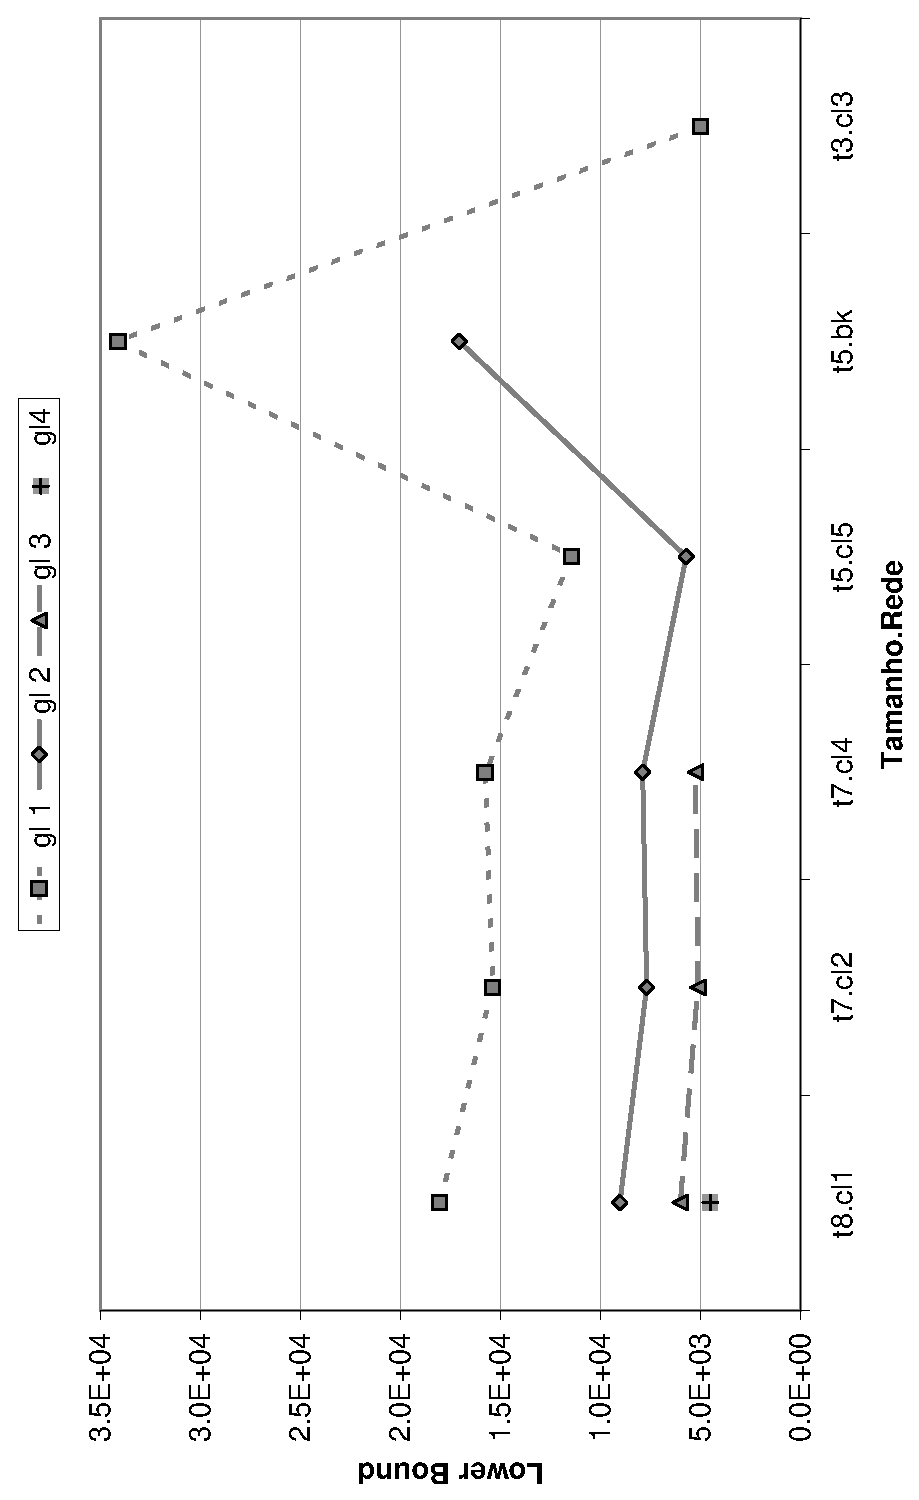
\includegraphics[angle=270,scale=.63]{./figs/cong.lb.eps}
 % cong.lb.eps: 595x842 pixel, 72dpi, 20.99x29.70 cm, bb=0 0 595 842
 \caption{\textit{Lower bounds} para o congestionamento.}
 \label{fig:cong.lb} 
\end{figure}

\begin{figure}[!htb]
 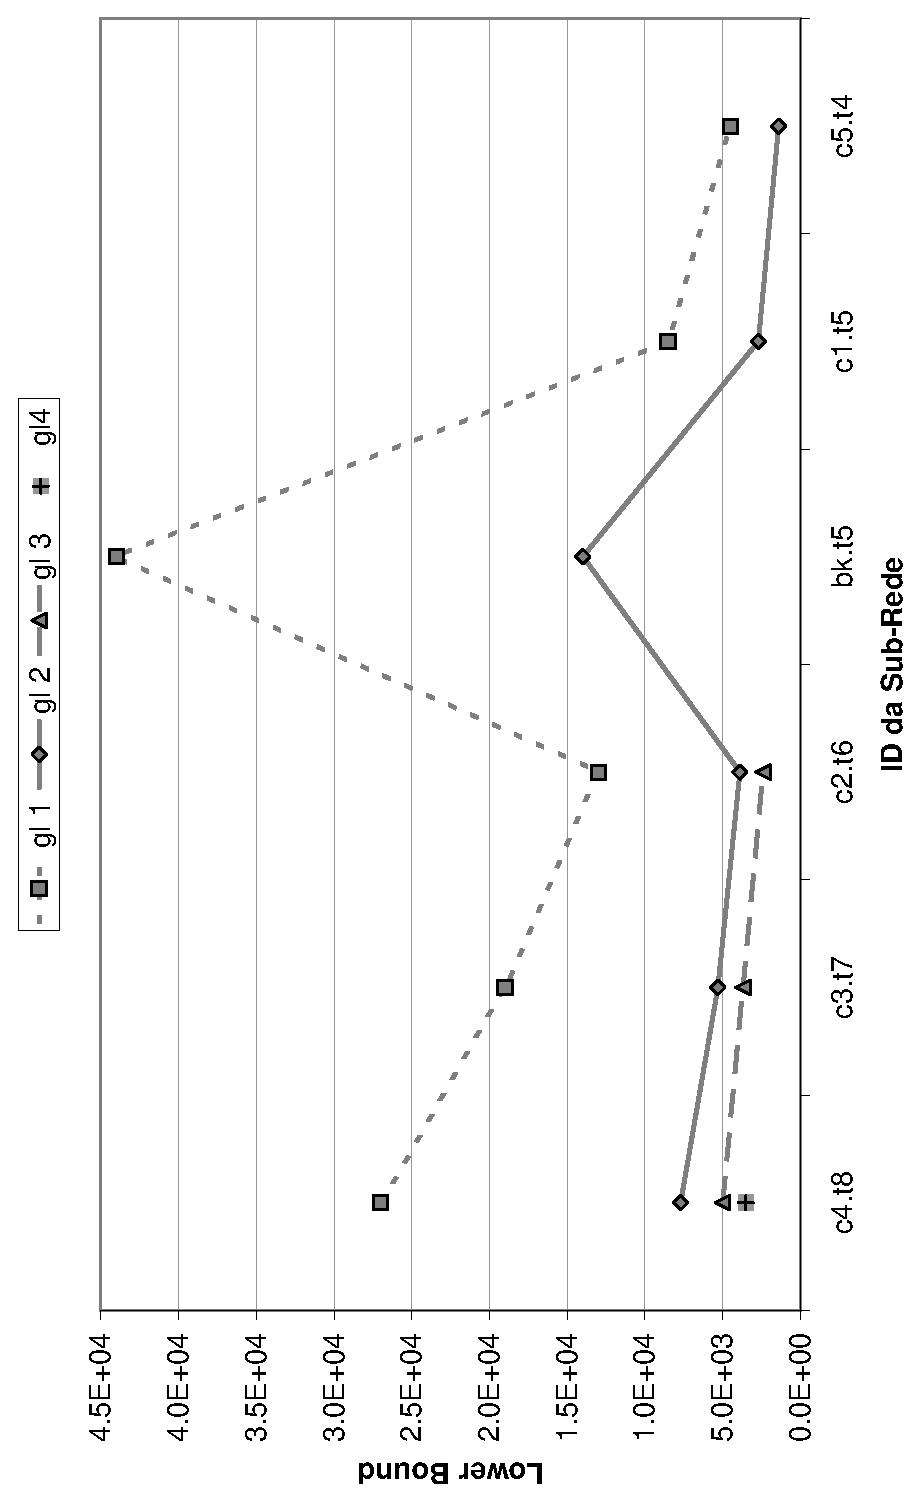
\includegraphics[angle=270,scale=.63]{./figs/traf.lb.eps}
 % traf.lb.eps: 595x842 pixel, 72dpi, 20.99x29.70 cm, bb=0 0 595 842
 \caption{\textit{Lower bounds} para o tr�fego retransmitido.}
 \label{fig:traf.lb} 
\end{figure}


A varia��o dos m�ximos e m�nimos amostrais para o tr�fego retransmitido, de acordo com o grau l�gico nas sub-redes, est� apresentada na figura
\ref{fig:traf.mm}.  Destaca-se a pequena diferen�a entre m�ximo e m�nimo para o caso de grau l�gico 1. Ainda para o tr�fego, a figura \ref{fig:traf.md.dp},
mostra o comportamento da m�dia e desvio padr�o. Mais uma vez observa-se a pouca varia��o no caso de grau l�gico 1, que � indicada pelo pequeno desvio padr�o.


\begin{figure}[htb!]
 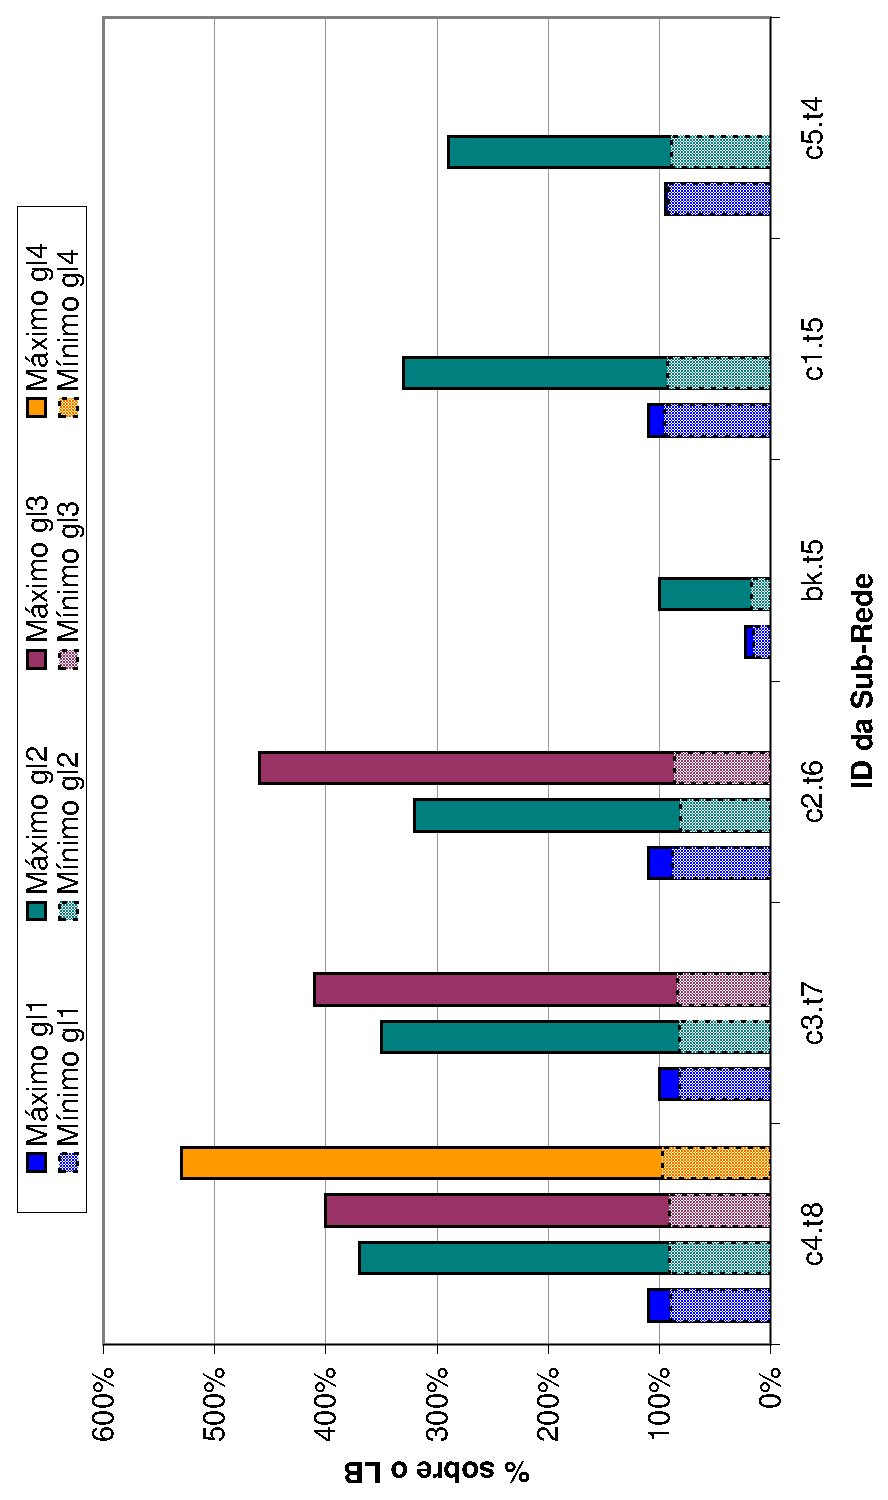
\includegraphics[angle=270,scale=.63]{./figs/traf.max.min.eps}
 % traf.gl1.max.min.eps: 595x842 pixel, 72dpi, 20.99x29.70 cm, bb=0 0 595 842
 \caption{M�ximo e m�nimo amostrais para o tr�fego retransmitido.}
 \label{fig:traf.mm}
\end{figure}

\begin{figure}[htb!]
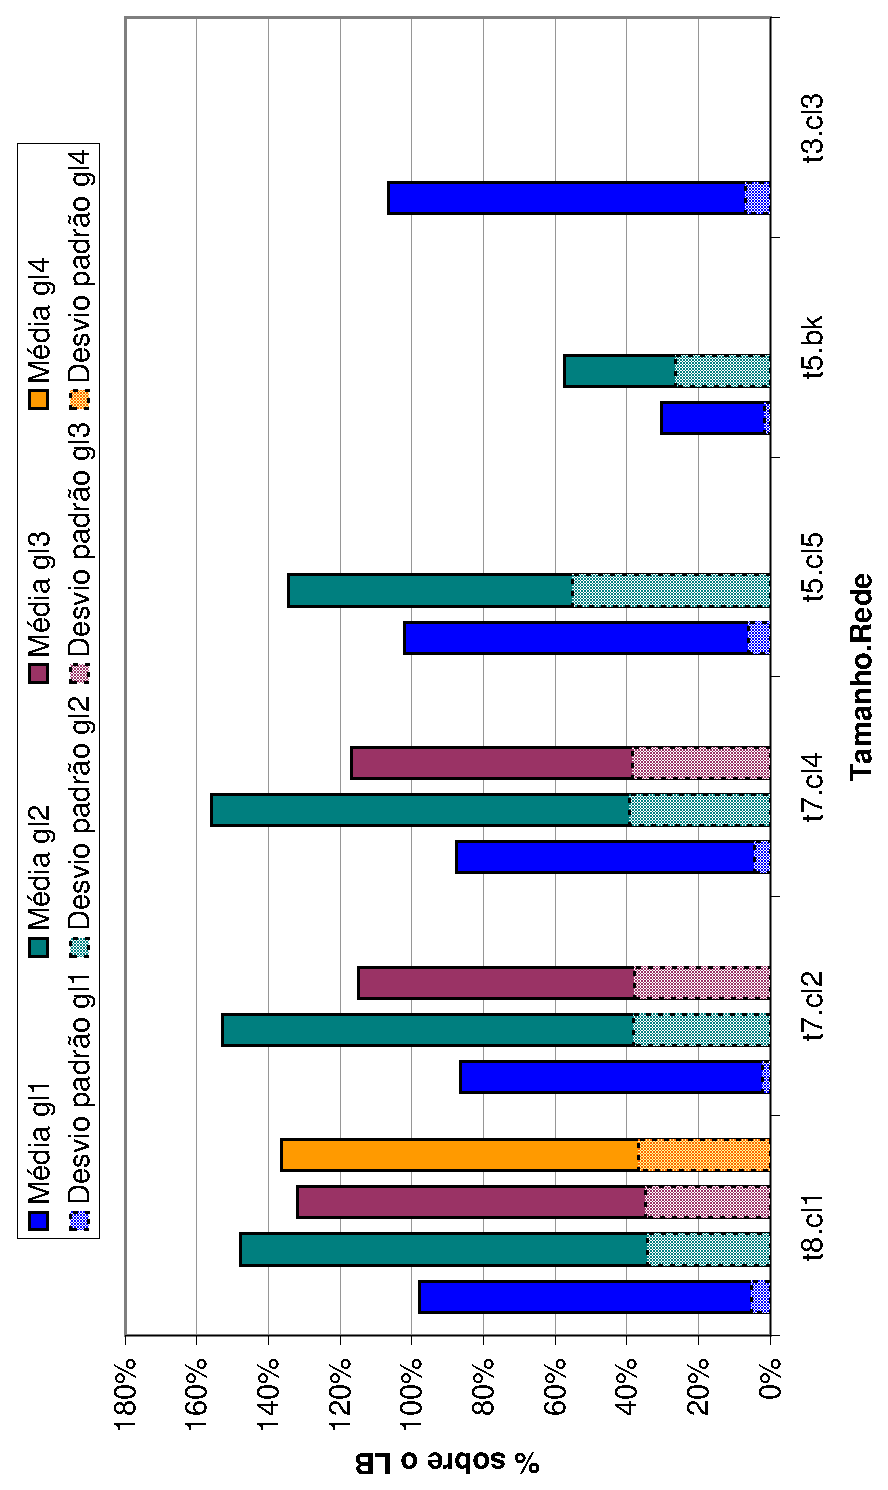
\includegraphics[angle=270,scale=.63]{./figs/traf.md.dp.eps}
\caption{M�dia e desvio padr�o amostrais para o tr�fego retransmitido.}
\label{fig:traf.md.dp}
\end{figure}

Conforme mencionado no cap�tulo anterior, o resultado principal dessa etapa de estima��o de estat�sticas para congestionamento e tr�fego retransmitido � a
defini��o de \textit{upper bounds} para os mesmos. A partir das estat�sticas obtidas pode-se definir uma regra para esses \textit{upper bounds} que
represente valores de boa qualidade para essas m�tricas. Os valores de \textit{upper bounds} definidos em fun��o das estat�sticas ser�o repassados para o
modelo TWA na etapa final do processo de resolu��o.

% Com base nas estat�sticas obtidas para o congestionamento, a regra adotada para seu \textit{upper bound} foi simplesmente a m�dia amostral. Isso se deve a
% pouca variabilidade das amostras. \underline{\textbf{Ap�s nova rodada de testes explicar melhor.}}


\begin{table}[!ht]
\begin{center}
\begin{tabular}{|cc|cc|}
\hline GL & ID & UBTRetr & Am\_UB \\
\hline 1 & t8.cl1 & 93\% & 17\% \\
1 & t7.cl2 & 84\% & 17\% \\
1 & t7.cl4 & 83\% & 21\% \\
1 & t5.cl5 & 96\% & 23\% \\
1 & t5.bk & 29\% & 24\% \\
1 & t3.cl3 & 100\% & 0\% \\
\hline 2 & t8.cl1 & 114\% & 10\% \\
2 & t7.cl2 & 115\% & 11\% \\
2 & t7.cl4 & 117\% & 10\% \\
2 & t5.cl5 & 79\% & 0\% \\
2 & t5.bk & 31\% & 2\% \\
\hline 3 & t8.cl1 & 97\% & 4\% \\
3 & t7.cl2 & 77\% & 0\% \\
3 & t7.cl4 & 78\% & 0\% \\
\hline 4 & t8.cl1 & 100\% & 1\% \\
\hline
\end{tabular}
\end{center}
\caption{Upper Bound para o tr�fego retransmitido e percentual de amostras que o atenderam.}
\label{tab:ub.traf}
\end{table}

Os \textit{upper bounds} foram definidos como a m�dia menos uma quantiade de desvios padr�o, para tanto o congestionamento ($HmDs$) quanto para o tr�fego
retransmitido ($TrDs$). Ambos s�o um m�ltiplo de $1/2$ e foram definidos como o m�ior poss�vel, desde que o \textit{upper bound} resultante n�o ultrapasse o
m�nimo amostral.

% Para o tr�fego retransmitido, a regra definida foi a m�dia amostral menos um desvio padr�o amostral. 
A tabela \ref{tab:ub.traf} mostra os valores resultantes
desta regra. Na terceira coluna, est�o os valores de \textit{upper bounds}, calculados em termos percentuais acima do respectivo \textit{lower bound}. A
�ltima coluna apresenta a propor��o de solu��es visitadas ao longo do processo de estima��o das estat�sticas, que apresentaram tr�fego retransmitido menor ou
igual ao \textit{upper bound}. Como pode-se notar, para grau l�gico 1, uma propor��o maior de solu��es atenderiam � regra. Outra constata��o � de que a medida
que o grau l�gico aumenta, essa propor��o � menor, independentemente do tamanho da sub-rede. Percebe-se tamb�m que no caso de malhas, grau l�gico superior a 1,
a regra definida localiza o \textit{upper bound} em valores bastante restritivos j� que no pior caso somente $11\%$ das solu��es visitadas atenderiam ao mesmo.
Para grau l�gico 1, caso particular onde a topologia virtual se resume a um anel, os valores mais altos para as propor��es de solu��es englobadas pelo
\textit{upper bound} podem ser explicados pelos resultados das estat�sticas, onde se observa uma pequena varia��o entre o m�ximo e o m�nimo amostral,
al�m de um pequeno desvio padr�o.



\section{Resolu��o das Sub-Redes com TWA}
\label{resultados:sec:twa}

Al�m dos par�metros de controle que obtemos a partir das estat�sticas, para garantir que a solu��o obtida para a topologia f�sica n�o seja muito dependente
da inst�ncia, como foi comentado na Se��o \ref{sec:subredes:custo_fisico}, calculamos a TIF para a rede NFSNET \cite{ram02}. O valor calculado foi $1.82$,
este ser� o valor de refer�ncia, sobre o qual ainda exigimos uma folga para baixo (\textit{TIFgap}), que variou entre $70\%$ e
$20\%$. Como iremos procurar solu��es resolvendo um modelo de programa��o linear inteira, nestes testes, n�o estamos utilizando a capacidade de TWA de
produzir solu��es com multiplas liga��es f�sicas, com o intuito de reduzir o n�mero de vari�veis bin�rias no modelo. 

Iniciamos com um \textit{TIFgap} de $40\%$ pois em testes piloto este se mostrou promissor. O \textit{TIFgap} foi reduzido nas situa��es em que n�o foi
poss�vel
encontrar solu��o vi�vel, e aumentado enquando ainda fossem encontradas solu��es.

Para cada \textit{TIFgap}, a estrat�gia adotada foi, partindo do menor grau l�gico ($Gl=1$), fixar nos valores m�nimos o n�mero de comprimentos de onda, e
executar o modelo b�sico do TWA, com as adi��es indicadas na Se��o \ref{sec:subredes:restricoes}. Um solver para problemas MILP � instanciado com essa
configura��o. Enquanto o solver retornar que o problema � insol�vel \cite{mukherjee}, $W$ ser� incrementado. 

Se o solver n�o encontrar uma solu��o vi�vel dentro de $10^4$ segundos, ent�o ele � abortado e � aplicado o mesmo precedimento de quando a
solu��o � insol�vel. Isso � feito com o objetivo de ``afrouxar'' as restri��es de modo que o solver possa encontrar uma solu��o vi�vel mais rapidamente, 
sacrificando um pouco a qualidade das restri��es. Essas situa��es em que o modelo precisou ser calibrado, que
chamaremos de \textit{Inst�ncia Insol�vel} ($I$), fazem parte do m�todo e s�o registradas conjuntamente com os resultados.

Se uma solu��o vi�vel � encontrada, o solver � interrompido,
a solu��o � registrada e o grau l�gico � incrementado, dando continuidade ao processo.

Como, nesta modelagem, $W$ est� diretamente relacionado a quantidade de vari�veis, � mais conveniente come�ar com $W=1$. Disso decorre a escolha 
de tamb�m come�armos com $Gl=1$. A maior prioridade para a incrementa��o � dada ao $Gl$, pois variando este temos inst�ncias diferentes. 
A menor preced�ncia ficou para $W$, pois quanto menor ele for menores precisar�o ser os custos de instala��o da rede.

Utilizamos o \textit{solver} SCIP (\textit{Solving Constraint Integer Programs} - scip.zib.de) para encontrar as solu��es vi�veis. Al�m de
calcular a capacidade dos canais �pticos ($Cap$), como foi descrito acima, o GLPK tamb�m foi usado para interpretar o modelo AMPL, gerando a
entrada de dados para o SCIP. Vale observar que o SCIP e o GLPK s�o \textit{softwares} livres, de c�digo fonte aberto e de distribui��o gratuita.

A tabela \ref{tab:cod.legenda2} apresenta as legendas para a tabela \ref{tab:result.twa}, que ser� utilizada na apresenta��o dos
resultados obtidos para o projeto completo das sub-redes utilizando o modelo TWA.% e \ref{tab:result.var.twa}

\begin{table}[!ht]
\begin{center}
\begin{tabular}{|ccc|}
\hline
GL & $=$ & Grau l�gico \\
ID & $=$ & Identifica��o da sub-rede \\
W & $=$ & N�mero de comprimentos de onda \\
TTranc & $=$ & Total de tranceptores \\
UBCong & $=$ & \textit{Upper bound} para congestionamento \\
UBTRetr & $=$ & \textit{Upper bound} para tr�fego retransmitido \\ 
UBCFis & $=$ & \textit{Upper bound} para custo f�sico \\
Cong & $=$ & Congestionamento \\
TRetr & $=$ & Tr�fego retransmitido \\
CFis & $=$ & Custo f�sico \\
t(s) & $=$ & Tempo de execu��o em segundos \\
Var\% & $=$ & Varia��o percentual \\
\hline
\end{tabular}
\end{center}
\caption{Legenda para as tabelas \ref{tab:result.twa}.} % e \ref{tab:result.var.twa}
\label{tab:cod.legenda2}
\end{table}



\begin{table}[!ht]
\begin{center}
\begin{tabular}{|cc|cc|ccc|ccc|c|}
\hline ID & GL & W & TTranc & UBCong & UBTRetr & UBCFis & Cong & TRetr & CFis & t(s)** \\
\hline t5.bk & 1 & 1 & 5 & 34140 & 50609 & 55 & & 50252 & 43 & 5 \\
t5.bk & 2 & 1 & 10 & 17070 & 15973 & 55 & & 15938 & 52 & 2 \\
\hline t3.cl3 & 1 & 1 & 3 & 4980 & 2406 & $\mathbf{106}$ & & 2406 & 104 & 0.02 \\
\hline t5.cl5 & 1 & 1 & 5 & 11443 & 16674 & $\mathbf{86}$ & & 16404 & 81 & 5 \\
t5.cl5 & 2 & 3 & 10 & 5723 & 5003 & 64 & & 3097 & 62 & 6 \\
\hline t7.cl2 & 1 & 1 & 7 & 15384 & 38016 & 89 & & 37553 & 87 & 16 \\
t7.cl2 & 2 & 1 & 11 & 7692 & 12067 & 89 & & 8973 & 86 & 4 \\
t7.cl2 & 3 & 2 & 16 & 5207 & 7057 & 89 & & 3476 & 89 & 9 \\
\hline t7.cl4 & 1 & 1 & 7 & 15776 & 38489 & 141 & & 37943 & 140 & 65 \\
t7.cl4 & 2 & 1 & 12 & 7888 & 12346 & 141 & & 11320 & 140 & 3 \\
t7.cl4 & 3 & 2 & 12 & 5338 & 7222 & 141 & & 7215 & 140 & 41 \\
\hline t8.cl1 & 1 & 1 & 8 & 18051 & 52733 & $\mathbf{157}$ & & 51930 & 141 & 1313 \\
t8.cl1 & 2 & 2 & 13 & 9025 & 16605 & 134 & & 14529 & 131 & 322 \\
t8.cl1 & 3 & 3 & 18 & 6058 & 10072 & 134 & & 9391 & 131 & 2349 \\
t8.cl1 & 4 & 4 & 19 & 4517 & 7260 & 134 & & 6640 & 134 & 141 \\
\hline
\end{tabular}
\end{center}
\caption{Resumo resultados TWA.}
\label{tab:result.twa}
\end{table}


A tabela \ref{tab:result.twa} apresenta os resultados obtidos com o TWA. Cada linha representa uma inst�ncia, composta por uma sub-rede e um grau l�gico.

Nas inst�ncias onde o n�mero de comprimentos de onda ($W$) necess�rio foi apenas $1$, significa que logo na primeira tentativa de resolu��o do modelo foi
poss�vel encontrar uma solu��o vi�vel que atendesse a todas as restri��es impostas. Nos demais casos, foi necess�rio incrementar $W$ e executar novamente o
experimento, at� encontrar uma solu��o vi�vel.

No modelo TWA o grau l�gico � representado como uma restri��o no n�mero total de tranceptores na rede e em cada n�. Como se trata de uma limita��o, existem
casos onde n�o s�o utilizados todos os tranceptores permitidos pelo grau l�gico definido. Como pode-se notar, al�m do grau l�gico $1$ onde � �bvio que o
n�mero de tranceptores deve ser igual ao n�mero de n�s, somente para o grau l�gico $2$ nas sub-redes de $5$ n�s foi necess�rio utilizar todos os
tranceptores permitidos, ou seja, o dobro do n�mero de n�s.

As colunas UBCong e UBTRetr representam os \textit{upper bounds} calculados a partir das estat�sticas de m�dia e desvio padr�o para congestionamento e tr�fego
retransmitido, conforme apresentado na se��o anterior.

Conforme descrito no in�cio desta se��o, a limita��o de custo f�sico foi definida com base na TIF da rede real NFSNET. Os valores da coluna UBCFis, foram
calculados a partir desse valor de refer�ncia para a TIF, menos um percentual (\textit{TIFgap}), que representa uma tentativa de for�ar uma boa qualidade no
resultado do projeto da rede f�sica. 

As tr�s colunas que seguem, Cong, TRetr e CFis, trazem os resultados obtidos para congestionamento, tr�fego retransmitido e custo f�sico, respectivamente.

Apesar do custo f�sico n�o possuir rela��o evidente com o grau l�gico, os experimentos mostraram que para grau l�gico $1$, topologia virtual em anel, o
mesmo pode ser mais exigido. Sendo este fato identificado pela necessidade de realizar ajustes para baixo no valor do \textit{TIFgap} adotado na TIF de
algumas
sub-redes.

Para duas inst�ncias, $c3.t7.gl1$ e $c1.t5.gl1$, mesmo com um \textit{TIFgap} de $0.0\%$ n�o foi poss�vel encontrar solu��o
vi�vel. Ent�o relaxamos os UBs para congestionamento e tr�fego retransmitido, reduzindo em $1/2$ o n�mero de desvios abaixo da m�dia para ambos, nas duas
inst�ncias. 


\begin{figure}[!htb]
 \includegraphics[angle=270,scale=.63]{./figs/twa.traf.eps}
 % twa.traf.eps: 595x842 pixel, 72dpi, 20.99x29.70 cm, bb=0 0 595 842
 \label{fig:twa.traf}
 \caption{Resultados para tr�fego retransmitido e de acesso ao \textit{backbone}.}
\end{figure}

A figura \ref{fig:twa.traf} mostra o comportamento do tr�fego retransmitido em cada sub-rede de acordo com o grau l�gico. Al�m disso, para evidenciar a solu��o
global da rede em hierarquia, ela destaca o tr�fego de acesso ao \textit{backbone} que foi calculado na etapa inicial, quando o Algoritmo Gen�tico fez a escolha
das sub-redes.


% \begin{table}[!ht]
% \begin{center}
% \begin{tabular}{|cc|cc|cc|cc|}
% \hline ID & GL & Cong & Var\% & CFis & Var\% & TRetr & Var\% \\
% \hline t5.bk & $1$ & & & $43$ & - & $50252$ & - \\
% t5.bk & $2$ & & & $52$ & $21\%$ & $15938$ & $-68\%$ \\
% %\hline t3.cl3 & $1$ & $104$ & - & $2407$ & - \\
% \hline t5.cl5 & $1$ & & & $81$ & - & $16404$ & - \\
% t5.cl5 & $2$ & & & $62$ & $-23\%$ & $3097$ & $-81\%$ \\
% \hline t7.cl2 & $1$ & & & $87$ & - & $37553$ & - \\
% t7.cl2 & $2$ & & & $86$ & $-1\%$ & $8973$ & $-76\%$ \\
% t7.cl2 & $3$ & & & $89$ & $3\%$ & $3476$ & $-61\%$ \\
% \hline t7.cl4 & $1$ & & & $140$ & - & $37943$ & - \\
% t7.cl4 & $2$ & & & $140$ & $0\%$ & $11320$ & $-70\%$ \\
% t7.cl4 & $3$ & & & $140$ & $0\%$ & $7215$ & $-36\%$ \\
% \hline t8.cl1 & $1$ & & & $141$ & - & $51930$ & - \\
% t8.cl1 & $2$ & & & $131$ & $-7\%$ & $14529$ & $-72\%$ \\
% t8.cl1 & $3$ & & & $131$ & $0\%$ & $9391$ & $-35\%$ \\
% t8.cl1 & $4$ & & & $134$ & $2\%$ & $6640$ & $-29\%$ \\
% \hline
% \end{tabular}
% \end{center}
% \caption{Comparativo varia��o \% TWA.}
% \label{tab:result.var.twa}
% \end{table}
% 
% 
% Para evidenciar a varia��o dos resultados, a tabela \ref{tab:result.var.twa} mostra em valores percentuais as diferen�as observadas para congestionamento,
% tr�fego retransmitido e custo f�sico. Observa-se que, como j� era de se esperar, n�o foi verificada correla��o entre o custo f��sico e o grau l�gico, mas sim
% com o tamanho da sub-rede. Com rela��o ao tr�fego retransmitido internamente nas sub-redes, observa-se que o mesmo decresce
% consideravelmente a medida que aumenta-se o grau l�gico.



%%%%%%%%%%%%%%%%%%%%%%%%%%%%%%%%%%%%%
%% Conclus�o
%% Copyright 2009 Marcelo de Oliveira Lima.
%% Este documento � distribu�do nos termos da licen�a 
%% GNU General Public License v2.
%%%%%%%%%%%%%%%%%%%%%%%%%%%%%%%%%%%%%


\chapter{Conclus�es}
\thispagestyle{empty}

Uma metodologia para o projeto completo de redes... foi apresentada, englobando os os problemas VTD e RWA, al�m da escolha da topologia f�sica da rede. Esta
formula��o � ... em rela��o as apresentadas na literatura e possui a vantagem de ...

Com uma complexidade computacional ...

A metodologia foi apresentado inicialmente ... contendo as restri��es e vari�veis consideradas essenciais para a resolu��o do projeto 
completo, que engloba a escolha da topologia f�sica, defini��o da topologia virtual, distribui��o de tr�fego, defini��o das rotas f�sicas e 
aloca��o dos comprimentos de onda. Nessa modelagem a fun��o objetivo adotada foi a minimiza��o do ....

Para validar experimentalmente a formula��o, foram realizados testes ..., aonde as redes consideradas possuem $xxx$, $xxx$ n�s. Os resultados obtidos
foram consideravelmente expressivos, com rela��o � qualidade das solu��es e ao desempenho computacional.

\textit{Para a rede de $14$ n�s foram feitos testes com duas matrizes de demandas de tr�fegos, que s�o inst�ncias cl�ssicas da literatura \cite{ram96}. Para
ambas
matrizes foram obtidos resultados melhores do que os encontrados na literatura para os par�metros controlados \cite{Sivarajan01}. Al�m disso, para $70\%$ das
inst�ncias foram obtidas solu��es �timas. O tempo demandado para produzir estes �ltimos resultados foi alto, em compara��o ao desempenho das heur�sticas
utilizadas na literatura \cite{Nina05}, todavia deve-se ressaltar o fato de que n�o foram utilizadas heur�sticas nem ferramentas comerciais.
}

O novo \textit{lower bound} para o tr�fego retransmitido foi introduzido neste trabalho, o \underline{\textbf{MTB}}, demostrou ser eficiente. \textit{Pois,
possui
demanda de tempo computacional desprez�vel, frente ao alto custo das t�cnicas conhecidas at� ent�o \cite{ram96}. Al�m disso, na maioria das inst�ncias em que
conseguimos provar a otimalidade ($62\%$), o MTB coincidiu com o �timo. E mesmo quando o MTB diferiu do �timo, no pior caso, ele ficou menos de $5\%$ abaixo
deste. Apenas este resultado j� muda o cen�rio para o problema VTD, tornando este um problema bem mais trat�vel. Uma vez que, obter bons resultados a partir de
heur�sticas n�o � tarefa dif�cil no VTD, conforme a literatura \cite{ram96}.}

A abrang�ncia da modelagem e o desempenho computacional obtido viabilizam, em trabalhos futuros, realizar....


%%%%%%%%%%%%%%%%%%%%%%%%%%%%%%%%%%%%%
%% Publica��es
%% Copyright 2009 Marcelo de Oliveira Lima.
%% Este documento � distribu�do nos termos da licen�a 
%% GNU General Public License v2.
%%%%%%%%%%%%%%%%%%%%%%%%%%%%%%%%%%%%%


\chapter*{Publica��es}
\thispagestyle{empty}

Rela��o da produ��o bibliogr�fica do autor desta disserta��o.

\begin{itemize}

\item \textbf{Artigos completos publicados em peri�dicos}


\begin{enumerate}

\item Lima, Marcelo de Oliveira; Lima, F. O.; Oliveira, E. S.; Segatto, M. E. V.. \textit{\textbf{Um Algoritmo H�brido para o Planejamento de Redes
�pticas}}. REIC - Revista Eletr�nica de Inicia��o Cient�fica, v. 4, p. 4, 2006. 

\end{enumerate}


\item \textbf{Trabalhos completos publicados em anais de congressos}

\begin{enumerate}

\item Lima, M. O.; Lima, F. O.; Segatto, M. E. V.; Almeida, R. T. R.; Oliveira, E. S.. \textit{\textbf{Projeto Completo de Redes �pticas em
Hierarquia}}. In: MOMAG 2010, 14� SBMO - Simp�sio Brasileiro de Microondas e Optoeletr�nica, 2010.

\item Lima, F. O.; Lima, M. O.; Segatto, M. E. V.; Almeida, R. T. R.. \textit{\textbf{Projeto Completo de Redes �pticas}}. In: MOMAG 2010, 14�
SBMO - Simp�sio Brasileiro de Microondas e Optoeletr�nica, 2010.

\item Lima, F. O.; Lima, M. O.; Segatto, M. E. V.; Almeida, R. T. R.; Oliveira, E. S.. \textit{\textbf{Um modelo eficiente para o projeto completo
de redes �pticas}}. In: XLI SBPO - Simp�sio Brasileiro de Pesquisa Operacional, 2009.

\item Silva, M. ; Paiva, M.; Lavagnoli, G.; Lima, M. O.; Segatto, M. E. V.; Oliveira, E. S.; Almeida, R. T. R.. \textit{\textbf{On
Solving HSHR Networks}}. In: 6th Conftele - Conference on Telecommunications, 2007. 

\item SILVA, M.; Paiva, M.; Lavagnoli, G.; Lima, M. O.; Segatto, M. E. V.; Almeida, R. T. R.; Oliveira, E. S.. \textit{\textbf{An�lise de
Redes �pticas em An�is Hier�rquicos}}. In: XXV SBrT - Simp�sio Brasileiro de Telecomunica��es, 2007. 

\item Segatto, M. E. V.; Oliveira, E. S.; Lima, M. O.; Lima, F. O.; Almeida, R. T. R.. \textit{\textbf{Hybrid approaches for the
design of mesh and hierarchical ring optical networks}}. In: Proceedings of SPIE06 - Photonics Europe 2006, v. 1. 

\item Lima, F. O.; Lima, M. O.; Oliveira, E. S.; Segatto, M. E. V.. \textit{\textbf{Reformulando o Problema de Projeto de An�is em Redes
�pticas}}. In: Proceedings of 4th ITS - International Information and Telecommunication Technologies Symposium, 2005.

\item Lima, M. O.; Oliveira, E. S.; Pereira, L. C. B.; Almeida, R. T. R.; Segatto, M. E. V.. \textit{\textbf{A Hybrid-Combined Algorithm
Approach for the Design Topologies and Flow Congestion Minimization of Optical Networks}}. In: Proceedings of the 5th Conference on Telecommunications -
Conftele, 2005. 

\item Lima, M. O.; Maioli, C.; Botelho, T.; Pereira, L. C. B.; Almeida, R. T. R.; Segatto, M. E. V.; Oliveira, E. S.. \textit{\textbf{The Design of Hierarchical
Self-Healing Rings Networks}}. In: Proceedings of the 5th Conference on Telecommunications - Conftele, 2005. 

\item Lima, M. O.; Oliveira, E. S.; Segatto, M. E. V.; Almeida, R. T. R.. \textit{\textbf{Projeto de Redes �pticas com Topologia em An�is
Hier�rquicos Tolerantes a Falhas}}. In: Anais do XXII Simp�sio Brasileiro de Telecomunica��es - SBrT 05, 2005. p. 1236-1237. 

\item Lima, M. O.; Oliveira, E. S.; Pereira, L. C. B.; Almeida, R. T. R.; Segatto, M. E. V.. \textit{\textbf{Estrat�gias com Algoritmos
H�bridos para Projeto de Redes �pticas}}. In: SBPO - Simp�sio Brasileiro de Pesquisa Operacional, 2004. 


\end{enumerate}


% \item \textbf{Resumos publicados em anais de congressos}
% 
% \begin{enumerate}
% 
% \item Lima, F. O.; Lima, Marcelo de Oliveira; Oliveira, E. S.; Segatto, M. E. V.. \textit{\textbf{O Problema de Projeto de An�is em Redes �pticas via
%Algoritmos para TSP}}. In: Anais do XXXVIII SBPO - Simp�sio Brasileiro de Pesquisa Operacional, 2006.
% 
% \end{enumerate}


\end{itemize}



\citeoption{abnt-show-options=no}
%\nocite{*}
%\bibliographystyle{abnt-alf}
%\bibliographystyle{abnt-num}
%\bibliographystyle{sbc}
\bibliography{biblio}


%%%%%%%%%%%%%%%%%%%%%%%%%%%%%%%%%%%%%
%% Revis�o das Teorias Utilizadas
%% Copyright 2009 Marcelo de Oliveira Lima.
%% Este documento � distribu�do nos termos da licen�a 
%% GNU General Public License v2.
%%%%%%%%%%%%%%%%%%%%%%%%%%%%%%%%%%%%%

\appendix
\chapter{Algoritmos Gen�ticos}
\label{ga}

Os algoritmos gen�ticos (\textit{GAs} - \textit{Genetic Algorithms}) s�o mecanismos de pesquisa baseados no processo de sele��o natural e na combina��o
gen�tica. Sua ideia
principal � fazer com que indiv�duos com certas caracter�sticas especiais, isto �, aqueles com mais afinidade com a fun��o de estudo, sobrevivam e se combinem.
Os
GAs utilizam processos de escolha e combina��o rand�micos, seguindo algumas regras probabil�sticas. Isto se deve ao fato de poder rastrear com menos v�nculos um
conjunto maior de indiv�duos evitando cair em converg�ncias a pontos de m�ximos e m�nimos locais \cite{ga1,ga2}.

O GA foi primeiro proposto por Holland (1975). � um m�todo de otimiza��o que opera sobre uma popula��o de indiv�duos, que representam poss�veis solu��es do
problema. A cada um � associada uma aptid�o ({\itshape fitness}) para a solu��o do problema em quest�o. As popula��es de indiv�duos s�o criadas e submetidas a
operadores gen�ticos: de sele��o, cruzamento ( {\itshape crossover}) e muta��o. Com base no {\itshape fitness }de cada indiv�duo, estes operadores geram um
processo de evolu��o natural dos mesmos. As poss�veis respostas geradas para o problema s�o vistas como indiv�duos que competir�o entre si pela oportunidade de
se
reproduzirem. Os mais aptos t�m maior chance de perpetuar parte de suas caracter�sticas, aumentando assim a probabilidade de se obter uma maior adapta��o da
popula��o em geral \cite{ga1}. Algumas vantagens dos GA's s�o seu alto grau de adaptabilidade e paralelismo.

Como exemplo, considere um problema do caixeiro viajante ou TSP, um dos problemas de roteamento mais tradicionais e conhecidos de programa��o
matem�tica \cite{tsp}. O TSP � descrito por um conjunto de $n$ cidades e uma matriz de dist�ncia entre elas, tendo o seguinte objetivo: o caixeiro viajante deve
sair, de uma cidade chamada origem, e visitar cada uma das $n$ cidades apenas uma �nica vez, retornando � cidade origem, percorrendo a menor dist�ncia poss�vel,
ou seja, deve ser encontrada uma rota fechada (ciclo hamiltoniano \cite{cormen02}) de comprimento m�nimo que passe exatamente uma �nica vez por cada cidade.
Na
Figura \ref{tsp} temos um exemplo de uma solu��o para um TSP de quatro cidades. Uma solu��o para um  TSP � uma combina��o das $n$ cidades que comp�em o
problema,
e cada permuta��o desta � outra solu��o.

\begin{figure}[ht]
\begin{center}
\includegraphics[scale=0.8]{figs/tsp.eps}
\end{center}
\caption{Exemplo de uma solu��o para um TSP de quatro cidades.}
\label{tsp}
\end{figure}

Considere um algoritmo gen�tico para um TSP de 6 cidades, com popula��o inicial que contenha as sequencias [123654] e [213645]. A partir de um processo de
sele��o
que leva em considera��o o melhor desempenho de um indiv�duo ao cumprimento da fun��o objetivo (no caso minimizar o percurso entre as cidades), grupos de
cromossomos par a par s�o escolhidos para reprodu��o. Num mecanismo de {\itshape crossover}, trocas de partes de seus genes s�o efetuadas e eventualmente
ocorrem
muta��es possibilitando a varia��o num�rica. Uma nova popula��o com isso � gerada e o processo � reiniciado. Seleciona-se aleatoriamente um ponto de ruptura da
sequencia (ponto de {\itshape crossing}), por exemplo, posi��o 3 : [123.654] e [213.645]. Permutando as duas partes dos cromossomos pais, cria-se uma pr�xima
gera��o ({\itshape offspring}) de indiv�duos : [123645] e [213654] que decodificados representam caminhos diferentes dos originais. Por sua vez se for efetuado
uma muta��o na sequencia [123645], permutando-se seus  dois �ltimos alelos obt�m-se [123654]. 

A codifica��o da informa��o em cromossomos � um ponto crucial durante o processo de modelagem do problema real, e junto com a fun��o objetivo, liga o GA ao
problema a ser resolvido. Se a codifica��o for feita de forma inteligente, essa j� incluir� as caracter�sticas do problema e permitir� que se evitem testes de
viabilidade de cada uma das solu��es geradas. No exemplo, se utilizarmos a posi��o 4 como ponto de {\itshape crossing}, ter�amos como resultado [123655] e
[213644] que n�o representa uma solu��o para o TSP, e eles dever�o ser descartados (lhes ser� atribu�do um {\itshape fitness }que os exclua do processo
evolutivo). Se a codifica��o n�o permitir esse tipo de anomalia, tais verifica��es ser�o desnecess�rias, melhorando assim o desempenho do algoritmo.

O modelo de cromossomos mais utilizado � a representa��o bin�ria, um vetor ou matriz de zeros e uns. Deste modo, uma codifica��o natural para uma topologia
virtual seria tomar a matriz de adjac�ncias como cromossomo. Entretanto, o GA pode gerar qualquer matriz de zeros e uns de mesma ordem o que pode gerar
topologias
invi�veis. Na Tabela \ref{matriz-anel-6} vemos uma matriz de adjac�ncias e sua respectiva topologia virtual na Figura \ref{anel-6}.

\begin{table}[!ht]
\begin{center}

\begin{tabular}{|c|c|c|c|c|c|}
\hline 0 & 1 & 0 & 0 & 0 & 0 \\
\hline 0 & 0 & 1 & 0 & 0 & 0 \\
\hline 0 & 0 & 0 & 1 & 0 & 0 \\
\hline 0 & 0 & 0 & 0 & 1 & 0 \\
\hline 0 & 0 & 0 & 0 & 0 & 1 \\
\hline 1 & 0 & 0 & 0 & 0 & 0 \\
\hline
\end{tabular}
\end{center}
\caption{Matriz de Adjac�ncias de um anel}
\label{matriz-anel-6}
\end{table}

\begin{figure}[!ht]
\centering
\includegraphics[scale=0.6]{figs/anel-6.eps}
\caption{Anel de 6 n�s}
\label{anel-6}
\end{figure}

Esta matriz poderia ser interpretada como um cromossomo bin�rio $6x6$, mas um indiv�duo que tivesse entradas n�o nulas na diagonal n�o poderia representar uma
topologia. Outro problema � a quest�o do grau l�gico; as entradas n�o nulas do cromossomo, em cada linha e coluna, n�o podem exceder o grau l�gico da rede. Al�m
de outras restri��es que podem ser consideradas, como o tipo de topologia (por exemplo, an�is). Mas, por outro lado, n�o importa ao GA como se codifica ou
decodifica a informa��o dos par�metros. Toda a informa��o relativa ao problema est� contida na fun��o objetivo do problema, que embute os m�dulos de codifica��o
e
decodifica��o dos par�metros. Deste modo, os operadores gen�ticos devem ser implementados de forma a n�o gerarem solu��es invi�veis, ou a fun��o objetivo dever�
estar apta a lidar com elas.

\chapter{Implementa��o de Algoritmos Gen�ticos}
\label{galib}

Diversas ferramentas para o aux�lio na implementa��o de um GA  encontram-se dispon�veis atualmente. Destaca-se a biblioteca GAlib \footnote{{\tt
http://lancet.mit.edu/ga/}} \cite{wall}, da linguagem de programa��o C++, que foi escolhida para trabalhar os GAs neste trabalho, por possuir v�rios algoritmos
implementados, al�m de ter licen�a livre e c�digo aberto. O que permite a utiliza��o dos objetos prontos, ao mesmo tempo em que possibilita a livre
adapta��o e complementa��o.

A GAlib � uma biblioteca multiplataforma (Unix, Linux, MacOS, Windows). Sua interface baseia-se em duas classes de objetos C++: o genoma ({\itshape genome}), e
o
GA ({\itshape genetic algorithm}). Cada objeto da classe {\itshape genome} � um indiv�duo da popula��o; uma solu��o para o problema. J� o objeto {\itshape
genetic
algorithm} define como a evolu��o ser� feita, utilizando uma fun��o objetivo (definida pelo usu�rio) respons�vel pela decodifica��o do genoma e atribui��o do
{\itshape fitness }aos indiv�duos \cite{wall}.

Utilizando os operadores (implementados no {\itshape genome}) e as estrat�gias de sele��o (implementados no {\itshape genetic algorithm}) s�o gerados novos
indiv�duos.  Para um algoritmo gen�tico simples, basta definir a representa��o (a maneira como uma solu��o ser� codificada em um genoma) a partir das classes de
genoma existentes, definir a fun��o objetivo e escolher um algoritmo gen�tico, dentre os oferecidos pela biblioteca, e talvez passar mais alguns par�metros,
como
crit�rios de parada e tamanho das popula��es. Novos genomas e operadores podem ser implementados pelo usu�rio para modificar um GA ou elaborar seu pr�prio
algoritmo. Um GA cont�m as caracter�sticas gerais do algoritmo e dos operadores, a estrat�gia de evolu��o, os par�metros de execu��o e o crit�rio de parada,
todos
personaliz�veis. 

A GAlib pode ser processada de maneira distribu�da, evoluindo popula��es e/ou indiv�duos paralelamente em  m�ltiplos CPUs. Os par�metros  do algoritmo gen�tico
podem ser configurados em arquivo, em linha de comando, e/ou no pr�prio c�digo. S�o suportados algoritmos com sobreposi��o de popula��o ({\itshape
Overlapping}),
nos quais se pode definir o n�mero de indiv�duos (ou uma porcentagem da popula��o) a ser mantida a cada gera��o. A documenta��o da biblioteca inclui exemplos de
outros algoritmos gen�ticos derivados, tais como um algoritmo gen�tico com sub popula��es e outros que usam aglomera��o determin�stica ({\itshape deterministic
crowding}). Dentre os crit�rios internos de parada est�o a converg�ncia e o n�mero de popula��es, que podem ser personalizados. 

Os cromossomos podem ser constru�dos de qualquer tipo de dados de C++. Pode-se usar os tipos internos � biblioteca ({\itshape bit-string, array, list, tree})
ou
criar um cromossomo baseado em seus pr�prios objetivos. Os tipos internos do cromossomo incluem {\itshape arrays }(arranjos), {\itshape list }(lista), {\itshape
tree} (�rvore), 1D, 2D, e 3D {\itshape arrays}, 1D, 2D, e 3D {\itshape binary string}. As listas e as �rvores podem conter todo tipo de objeto em seus n�s, bem
como os arranjos em cada um de seus elementos. A biblioteca contem quatro tipos de genomas:  {\itshape GAListGenome, GATreeGenome, GAArrayGenome}, e {\itshape
GABinaryStringGenome}.  Estas classes s�o derivadas da classe b�sica GAGenome e de uma classe de estrutura de dados como indicado por seus nomes (por exemplo, o
{\itshape GAListGenome} � derivado das classes {\itshape GAList }e {\itshape GAGenome}).  Por exemplo, se estiver tentando otimizar uma fun��o que dependa de 5
n�meros reais, use ent�o como seu genoma um arranjo de uma dimens�o de n�meros reais com 5 elementos.

H� muitos tipos diferentes de algoritmos gen�ticos.  A biblioteca GAlib inclui tr�s tipos b�sicos:  {\itshape simple,  steady-state, e incremental}.  Estes
algoritmos diferem na maneira como criam indiv�duos novos e substituem indiv�duos velhos durante uma evolu��o. Esta biblioteca ainda fornece dois mecanismos
preliminares que estendem as potencialidades dos objetos internos.  Um recurso bastante utilizado � a defini��o de classes personalizadas com novas fun��es
membro.  Mas, se houver necessidade de fazer somente ajustes menores ao comportamento de uma classe GAlib, na maioria dos casos pode-se definir uma �nica fun��o
e
dizer � classe existente para us�-la ao inv�s do {\itshape default}.


\chapter{Estima��o de Par�metros}

... Falta escrever.




% \pretextualchapter{}
\chapter*{Ferramentas Computacionais}
\label{cap:ferramentas}
% \newpage


As ferramentas computacionais envolvidas neste trabalho, listadas abaixo, s�o distribu�das sob licen�as de C�digo Livre (\textit{Open Source}). O c�digo
fonte $\LaTeX$ desta disserta��o e todo o trabalho desenvolvido est� dispon�vel em \url{http://code.google.com/p/twa}. 

Todas as figuras incluidas neste texto foram criadas em SVG
(\textit{Scalable Vectorial Graphics} - \url{http://w3.org/Graphics/SVG}) e convertidas para o formato EPS (\textit{Encapsulated PostScript} -
\url{http://adobe.com/products/postscript}) para posterior inclus�o no c�digo $\LaTeX$, ambos formatos abertos. A Figura \ref{fig:nsfnet}, criada pelo autor
deste
texto, est� registrada em \url{http://wikimedia.org/wiki/File:NSFNET_14nodes.svg}.

\begin{itemize}
   \item Kubuntu GNU/Linux: a vers�o 9.10 foi usada na esta��o de trabalho e a vers�o 9.04 no servidor aonde foram
executados os testes computacionais. 
\url{http://kubuntu.org}

   \item GLPK 4.37 - \textit{GNU Linear Programming Kit}: usado para resolver modelos de programa��o inteira e converter c�digo AMPL em FreeMPS.
\url{http://gnu.org/software/glpk}

   \item SCIP - \textit{Solving Constraint Integer Programs}, vers�o 1.1.0 Linux X86: usado para resolver os modelos de programa��o interira mista.
\url{http://scip.zib.de}

   \item CLP 1.11 - \textit{Coin-or Linear Programming}: usado internamente pelo SCIP para resolver subproblemas de programa��o linear.
\url{http://coin-or.org}

   \item TexLive 2007: distribui��o $\LaTeX$ utilizada para a confec��o desta disserta��o.\\
\url{http://tug.org/texlive}

   \item Kile 2.0.83: editor de texto com ferramentas para autoria em $\LaTeX$ utilizado. \\
\url{http://kile.sourceforge.net}

   \item Inkscape 0.47: editor de desenho vetorial utilizado para criar as figuras SVG e convert�-las em EPS. 
\url{http://inkscape.org}

\end{itemize}
 

% \vspace{2cm}
% \vspace{5cm}

\begin{center}
\textbf{Feito em} \\
\textbf{$\LaTeX$}
\end{center}


\end{document}

